\documentclass[a4paper]{report}

\usepackage[top=2cm, bottom=2cm, left=1.5cm, right=1.5cm]{geometry}
\geometry{a4paper}
\usepackage[utf8]{inputenc}
\DeclareUnicodeCharacter{2212}{\textendash}
\usepackage[toc,page]{appendix}
\usepackage{bm}
\usepackage{amssymb}
\usepackage{amsmath}
\usepackage{amsthm}
\usepackage{mathtools}
\usepackage{graphicx}
\usepackage{caption}
\usepackage{subcaption}
\usepackage{xcolor}
\usepackage[many]{tcolorbox}
\usepackage[Glenn]{fncychap}
\usepackage{diagbox}
\usepackage{csquotes}
\usepackage{placeins}
\usepackage[numbers]{natbib}
\usepackage[colorlinks=true, linkcolor=blue, urlcolor=blue,
            citecolor=blue]{hyperref}
\usepackage{bookmark}

\newtheorem{theorem}{Theorem}
\newtheorem{proposition}{Proposition}

\definecolor{codegray}{gray}{0.9}
\newcommand{\code}[1]{\colorbox{codegray}{\texttt{#1}}}
\newcommand{\indep}{\perp\!\!\!\perp}
\newcommand{\KL}{\mathrm{KL}}
\newcommand{\E}{\mathbb{E}}

% Remarks in the author's voice (kept from the original report)
\newtcolorbox{story}[1][]{
    width=\textwidth,
    colback=magenta!10,
    colframe=black!40,
    colbacktitle=blue!30,
    fonttitle=\bfseries,
    left=1ex, right=1ex, top=2pt,
    arc=0pt, outer arc=0pt,
    leftrule=0pt, rightrule=0pt, toprule=0pt, bottomrule=0pt,
    breakable, enhanced jigsaw,
    title={#1}}

% Plain-language explanation of a formula or a result
\newtcolorbox{inwords}[1][In words]{
    width=\textwidth,
    colback=teal!6,
    colframe=teal!55!black,
    fonttitle=\bfseries,
    left=1ex, right=1ex, top=2pt,
    arc=2pt, boxrule=0.6pt,
    breakable, enhanced jigsaw,
    title={#1}}

% Annexes: sections numbered I, II, ... (appendices are lettered A, B, ...)
\newcommand{\annexes}{
    \chapter*{Annex}
    \addcontentsline{toc}{chapter}{Annex}
    \setcounter{section}{0}
    \setcounter{subsection}{0}
    \renewcommand{\thesection}{\Roman{section}}
    \renewcommand{\thesubsection}{\thesection.\arabic{subsection}}
}

\makeatletter
\def\@makechapterhead#1{%
  {\parindent \z@ \raggedright \normalfont
    \ifnum \c@secnumdepth >\m@ne
        \huge\bfseries \@chapapp\space \thechapter
        \par\nobreak
        \vskip 20\p@
    \fi
    \interlinepenalty\@M
    \Huge \bfseries #1\par\nobreak
    \vskip 20\p@
  }}
\makeatother

\begin{document}

\fontsize{11pt}{13pt}\selectfont

\begin{titlepage}
    \centering
    \vspace*{0.5cm}
    {\Huge \textbf{Deep Kalman Filters}} \\
    \vspace{0.4cm}
    \vspace{1cm}
    {\Large Christophe Louargant} \\
    \vspace{0.5cm}
    {\LARGE \textbf{C}onservatoire \textbf{N}ational des \textbf{A}rts
    et \textbf{M}étiers} \\
    \vspace{0.5cm}
    {\Large \textbf{Paris}}\\
    \vspace{1.5cm}
    {\Large RCP 217} \\
    \vspace{0.6cm}
    {\large December 2024} \\
    \vspace{1cm}
    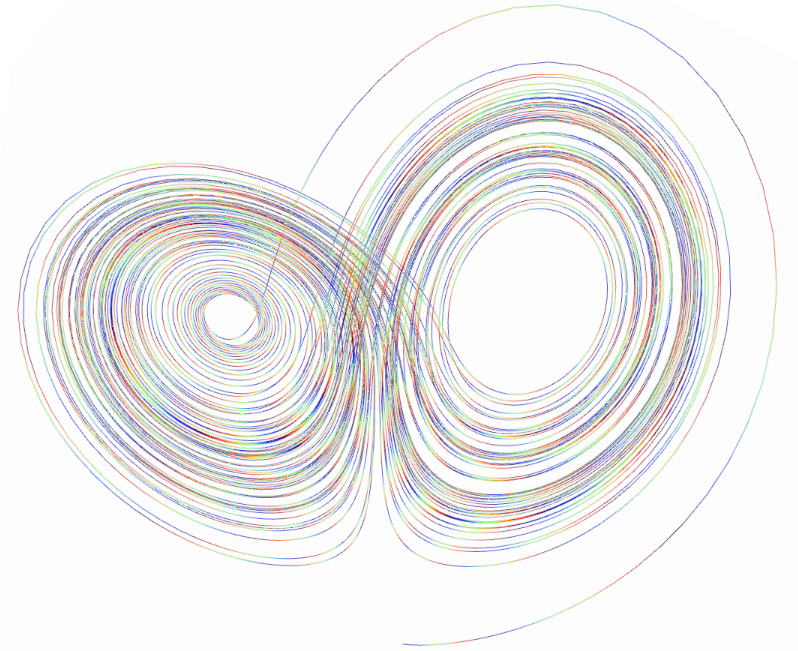
\includegraphics[width=0.9\textwidth]{./Images/lorenz_attractor_color.png}
    \vfill
    \section*{License}
    This work is licensed under the Creative Commons
    Attribution 4.0 International License.
\end{titlepage}

\tableofcontents
\listoffigures

\newpage

\chapter{Introduction}

The Deep Kalman Filter (DKF), introduced by Krishnan, Shalit and Sontag
in 2015 \cite{krishnan2015deep}, is a sequential latent-variable model.
It keeps the structure of the Kalman filter, a latent state that evolves
as a Markov chain and emits one observation per time step, but replaces
the linear-Gaussian transition and emission models by Gaussian
distributions whose parameters are computed by neural networks. Since
exact posterior inference is then intractable, the model is trained like
a Variational Auto-Encoder (VAE): an inference network approximates the
posterior over the latent trajectory, and the parameters of both networks
are learned jointly by maximising the Evidence Lower Bound (ELBO).\\

This report presents the mathematics of the DKF, my implementation of
it\footnote{The code is available
\href{https://github.com/CL-BZH/Deep-Kalman-Filters/tree/main}{on
GitHub}.}, and experiments on noisy sine waves and on sequences generated
by the Lorenz attractor\footnote{The cover page shows a realisation of
the Lorenz attractor used to test the models.}. It is organised as
follows.
\begin{itemize}
    \item Chapter 2 recalls the Kalman filter. It is the linear-Gaussian
    special case in which the posterior that the DKF approximates can be
    computed exactly.
    \item Chapter 3 recalls the VAE and, in particular, \emph{why} the
    ELBO is a lower bound on the log-likelihood.
    \item Chapter 4 is the core of the report: the DKF model, the
    structure of its true posterior (derived with d-separation), the
    factorised ELBO, how that ELBO is estimated by sampling, the
    implementation, and three extensions I designed: the autoregressive
    DKF (AR DKF) and its two variants FAR DKF and BAR DKF.
    \item The appendices give the complete derivations and the
    experimental results. The annex recalls d-separation.
\end{itemize}

\chapter{Kalman Filter}\label{chap:kalman}

\section{Introduction}

The Kalman filter estimates the state of a linear dynamical system from a
sequence of noisy measurements. In the robotics and signal-processing
literature the state at time $t$ is usually written $\mathbf{x}_t$ and
the measurement $\mathbf{z}_t$ (see, e.g., \cite{thrun2005probabilistic}).
The Deep Kalman Filter paper \cite{krishnan2015deep} follows the VAE
convention instead, and I do the same throughout this report:
$\mathbf{z}_t$ is the \emph{latent} state and $\mathbf{x}_t$ the
\emph{observed} measurement.

\begin{story}[Control input $\mathbf{u}_{t-1}$ versus $\mathbf{u}_{t}$]
Krishnan et al.\ write the control input that drives the transition from
$t-1$ to $t$ as $\mathbf{u}_{t-1}$, but when they define their
variational models, $\mathbf{u}_{t}$ is synchronous with
$\mathbf{z}_{t}$. I keep the convention of the Kalman-filter literature
and write $\mathbf{u}_{t}$ for the input acting on the transition into
$\mathbf{z}_{t}$. This is only a matter of indexing.
\end{story}

\section{System Model}

The system is described by an initial belief, a state-transition
equation and an observation equation.

\paragraph{Initial state.}
$\mathbf{z}_{0} \sim \mathcal{N}(\boldsymbol{\mu}_{0},
\boldsymbol{\Sigma}_{0})$.

\paragraph{State transition.} For $t \geq 1$,
\begin{equation*}
    \mathbf{z}_t = \mathbf{G}_t \mathbf{z}_{t-1} + \mathbf{B}_t
    \mathbf{u}_t + \boldsymbol{\varepsilon}_t,
    \qquad
    \boldsymbol{\varepsilon}_t \sim \mathcal{N}(\mathbf{0},
    \boldsymbol{\Sigma}_{t}),
\end{equation*}
where $\mathbf{G}_t$ is the state-transition matrix, $\mathbf{B}_t$ the
control-input matrix, $\mathbf{u}_t$ the (known) control input and
$\boldsymbol{\varepsilon}_t$ the process noise. Equivalently,
\begin{equation}
    p(\mathbf{z}_t \mid \mathbf{z}_{t-1}, \mathbf{u}_t) =
    \mathcal{N}(\mathbf{z}_t;\ \mathbf{G}_t \mathbf{z}_{t-1} +
    \mathbf{B}_t \mathbf{u}_t,\ \boldsymbol{\Sigma}_{t}).
    \label{eq:1}
\end{equation}

\paragraph{Observation.} For $t \geq 1$,
\begin{equation*}
    \mathbf{x}_t = \mathbf{F}_t \mathbf{z}_t + \boldsymbol{\eta}_t,
    \qquad
    \boldsymbol{\eta}_t \sim \mathcal{N}(\mathbf{0},
    \boldsymbol{\Gamma}_{t}),
\end{equation*}
where $\mathbf{F}_t$ is the observation matrix and
$\boldsymbol{\eta}_t$ the measurement noise. Equivalently,
\begin{equation}
    p(\mathbf{x}_t \mid \mathbf{z}_t) =
    \mathcal{N}(\mathbf{x}_t;\ \mathbf{F}_t \mathbf{z}_{t},\
    \boldsymbol{\Gamma}_{t}).
    \label{eq:2}
\end{equation}

\section{Kalman Filter Algorithm}

Write $\hat{\mathbf{z}}_{t}$ and $\mathbf{P}_{t}$ for the mean and
covariance of the state given the measurements up to time $t$. The filter
alternates two steps.

\subsection{Prediction Step}
\begin{itemize}
    \item \textbf{Predicted (a priori) mean:}\quad
    $\bar{\mathbf{z}}_{t} = \mathbf{G}_t \hat{\mathbf{z}}_{t-1} +
    \mathbf{B}_t \mathbf{u}_t$.
    \item \textbf{Predicted (a priori) covariance:}\quad
    $\bar{\mathbf{P}}_{t} = \mathbf{G}_t \mathbf{P}_{t-1}
    \mathbf{G}_t^\top + \boldsymbol{\Sigma}_{t}$.
\end{itemize}
These are the mean and covariance of the state at time $t$ given the
measurements up to time $t-1$.

\subsection{Update Step}
\begin{itemize}
    \item \textbf{Innovation (measurement residual):}\quad
    $\mathbf{y}_t = \mathbf{x}_t - \mathbf{F}_t \bar{\mathbf{z}}_{t}$.
    \item \textbf{Innovation covariance:}\quad
    $\mathbf{S}_t = \mathbf{F}_t \bar{\mathbf{P}}_{t} \mathbf{F}_t^\top
    + \boldsymbol{\Gamma}_{t}$.
    \item \textbf{Kalman gain:}\quad
    $\mathbf{K}_t = \bar{\mathbf{P}}_{t} \mathbf{F}_t^\top
    \mathbf{S}_t^{-1}$.
    \item \textbf{Updated (a posteriori) mean:}\quad
    $\hat{\mathbf{z}}_{t} = \bar{\mathbf{z}}_{t} + \mathbf{K}_t
    \mathbf{y}_t$.
    \item \textbf{Updated (a posteriori) covariance:}\quad
    $\mathbf{P}_{t} = (\mathbf{I} - \mathbf{K}_t \mathbf{F}_t)
    \bar{\mathbf{P}}_{t}$.
\end{itemize}

\section{The probabilistic reading of the Kalman filter}

Because every distribution in the model is Gaussian and every map is
linear, all posterior distributions are Gaussian and can be computed in
closed form. The two steps above compute exactly
\begin{equation*}
    p(\mathbf{z}_t \mid \mathbf{x}_{1:t-1}, \mathbf{u}_{1:t}) =
    \mathcal{N}(\bar{\mathbf{z}}_{t}, \bar{\mathbf{P}}_{t})
    \qquad\text{and}\qquad
    p(\mathbf{z}_t \mid \mathbf{x}_{1:t}, \mathbf{u}_{1:t}) =
    \mathcal{N}(\hat{\mathbf{z}}_{t}, \mathbf{P}_{t}).
\end{equation*}
The innovations also give the exact log-likelihood of the measurements,
\begin{equation*}
    \log p(\mathbf{x}_{1:T} \mid \mathbf{u}_{1:T}) =
    \sum_{t=1}^{T} \log \mathcal{N}(\mathbf{y}_t;\ \mathbf{0},\
    \mathbf{S}_t),
\end{equation*}
and a backward pass (the Rauch--Tung--Striebel smoother) gives the
\emph{smoothing} distributions
$p(\mathbf{z}_t \mid \mathbf{x}_{1:T}, \mathbf{u}_{1:T})$, which use the
future measurements as well.

\begin{inwords}
In the linear-Gaussian case, \enquote{filtering} and \enquote{smoothing}
are exact Bayesian inference, done with matrix algebra. The Deep Kalman
Filter keeps the same probabilistic structure but makes the transition
and emission non-linear. Then none of these distributions has a closed
form any more. The DKF replaces exact inference by a neural network that
\emph{approximates} the smoothing posterior, and replaces the exact
log-likelihood by a lower bound on it. Chapters~\ref{chap:vae} and
\ref{chap:dkf} explain how.
\end{inwords}

\section{Summary}

The Kalman filter alternates a prediction step, which propagates the
belief through the dynamics, and an update step, which corrects it with
the new measurement. For linear-Gaussian systems this is exact inference,
and the resulting estimate is optimal in the mean-squared-error sense.
The Deep Kalman Filter replaces all the linear maps by non-linear maps
parameterised by neural networks, at the price of approximate inference.

\chapter{Overview of VAEs}\label{chap:vae}

\section{Introduction}

This chapter recalls the Variational Auto-Encoder (VAE) and introduces
the notions used for the Deep Kalman Filter in the next chapter. For a
complete treatment, see Murphy's book \cite{murphy2023probabilistic}.

A VAE has two components (Figure~\ref{fig:vae}):
\begin{itemize}
    \item an \textbf{encoder}, which maps an input
    $\textcolor{red}{\mathbf{x}}$ to a distribution over a latent variable
    $\textcolor{green!50!black}{\mathbf{z}}$;
    \item a \textbf{decoder}, which maps a latent value
    $\textcolor{green!50!black}{\mathbf{z}}$ to a distribution over the
    data space, from which a reconstruction
    $\textcolor{red}{\hat{\mathbf{x}}}$ is obtained.
\end{itemize}

\begin{figure}[ht!]
    \centering
    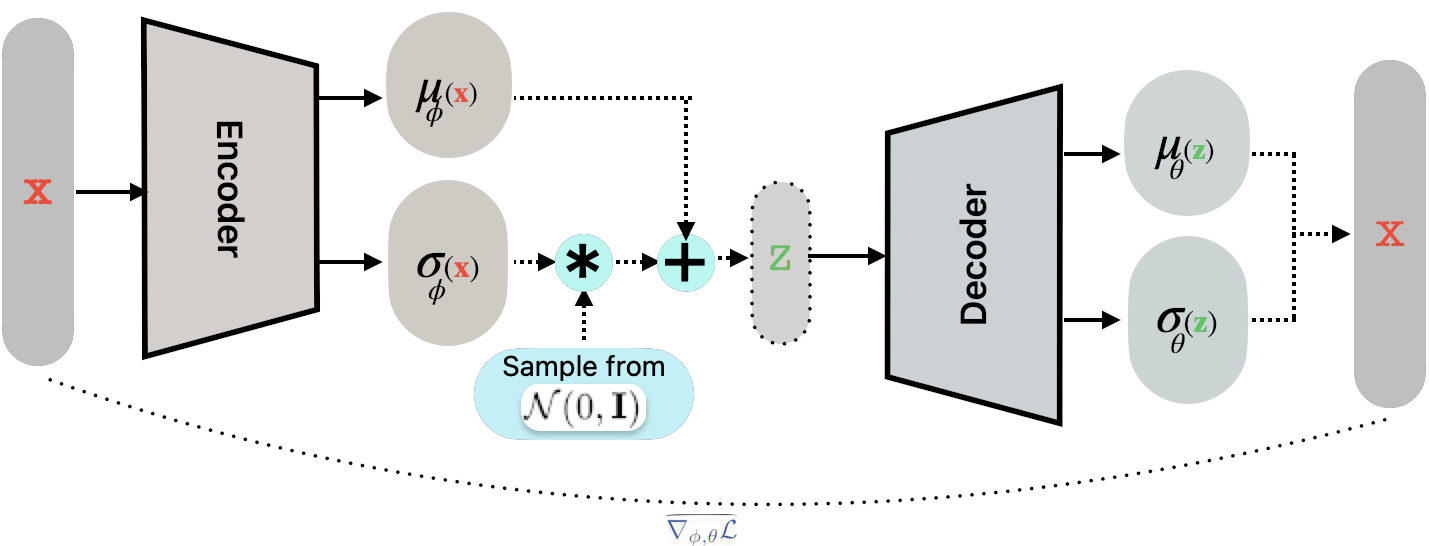
\includegraphics[width=300px]{./Images/vae.png}
    \caption{Variational Auto-Encoder}
    \label{fig:vae}
\end{figure}

\section{The model}

Let $\{\mathbf{x}^{(1)}, \dots, \mathbf{x}^{(N)}\}$ be a dataset of
independent data points. Each data point is assumed to be generated by
the following process.

\paragraph{Generative model (decoder).}
\begin{equation*}
    p(\mathbf{z}) = \mathcal{N}(\mathbf{z};\ \mathbf{0}, \mathbf{I}),
    \qquad
    p_{\theta}(\mathbf{x} \mid \mathbf{z}) =
    \mathcal{N}\big(\mathbf{x};\ \boldsymbol{\mu}_{\theta}(\mathbf{z}),\
    \mathrm{diag}(\boldsymbol{\sigma}^2_{\theta}(\mathbf{z}))\big),
\end{equation*}
where $\boldsymbol{\mu}_{\theta}$ and $\boldsymbol{\sigma}^2_{\theta}$
are computed by a neural network with parameters $\theta$.

\paragraph{Inference model (encoder).}
The posterior
$p_\theta(\mathbf{z} \mid \mathbf{x}) =
p_\theta(\mathbf{x} \mid \mathbf{z})\,p(\mathbf{z})/p_\theta(\mathbf{x})$
is intractable, because
$p_\theta(\mathbf{x}) = \int p_\theta(\mathbf{x} \mid \mathbf{z})\,
p(\mathbf{z})\,d\mathbf{z}$ has no closed form when the decoder is a
neural network. It is approximated by
\begin{equation*}
    q_{\phi}(\mathbf{z} \mid \mathbf{x}) =
    \mathcal{N}\big(\mathbf{z};\ \boldsymbol{\mu}_{\phi}(\mathbf{x}),\
    \mathrm{diag}(\boldsymbol{\sigma}^2_{\phi}(\mathbf{x}))\big),
\end{equation*}
where $\boldsymbol{\mu}_{\phi}$ and $\boldsymbol{\sigma}^2_{\phi}$ are
computed by a second neural network with parameters $\phi$. A single
network serves every data point; this is called \emph{amortised}
inference.

\section{The Evidence Lower Bound}

\subsection{Why it is a lower bound}

For any distribution $q(\mathbf{z} \mid \mathbf{x})$ whose support
contains that of the posterior,
\begin{align*}
    \log p_\theta(\mathbf{x})
    &= \log \int q(\mathbf{z} \mid \mathbf{x})\,
       \frac{p_\theta(\mathbf{x}, \mathbf{z})}{q(\mathbf{z} \mid
       \mathbf{x})}\,d\mathbf{z}
     = \log \E_{q(\mathbf{z} \mid \mathbf{x})}\!\left[
       \frac{p_\theta(\mathbf{x}, \mathbf{z})}{q(\mathbf{z} \mid
       \mathbf{x})}\right] \\
    &\geq \E_{q(\mathbf{z} \mid \mathbf{x})}\!\left[\log
       \frac{p_\theta(\mathbf{x}, \mathbf{z})}{q(\mathbf{z} \mid
       \mathbf{x})}\right] \;=:\; \mathcal{L}(\theta, \phi; \mathbf{x}),
\end{align*}
by Jensen's inequality, since $\log$ is concave. This is the
\textbf{Evidence Lower Bound} (ELBO). The size of the gap is known
exactly. Writing
$p_\theta(\mathbf{x}, \mathbf{z}) = p_\theta(\mathbf{x})\,
p_\theta(\mathbf{z} \mid \mathbf{x})$ inside the logarithm gives
\begin{equation}
    \log p_\theta(\mathbf{x}) = \mathcal{L}(\theta, \phi; \mathbf{x}) +
    \KL\big(q_\phi(\mathbf{z} \mid \mathbf{x}) \,\|\,
    p_\theta(\mathbf{z} \mid \mathbf{x})\big).
    \label{eq:elbo_gap}
\end{equation}

\begin{inwords}
The ELBO is below the log-likelihood by exactly the KL divergence
between the encoder and the true posterior. Maximising the ELBO over
$\phi$ therefore makes the encoder a better approximation of the
posterior. Maximising it over $\theta$ pushes the log-likelihood up.
The bound is tight when the encoder equals the posterior.
\end{inwords}

\subsection{Reconstruction and regularisation terms}

Writing $p_\theta(\mathbf{x}, \mathbf{z}) =
p_\theta(\mathbf{x} \mid \mathbf{z})\,p(\mathbf{z})$ instead gives the
usual form
\begin{equation*}
    \mathcal{L}(\theta, \phi; \mathbf{x}) =
    \underbrace{\E_{q_{\phi}(\mathbf{z} \mid \mathbf{x})}
    \big[\log p_{\theta}(\mathbf{x} \mid \mathbf{z})\big]}_{
    \text{reconstruction term}}
    \;-\;
    \underbrace{\KL\big(q_{\phi}(\mathbf{z} \mid \mathbf{x}) \,\|\,
    p(\mathbf{z})\big)}_{\text{regularisation term}}.
\end{equation*}
\begin{itemize}
    \item The \textbf{reconstruction term} rewards latent codes from
    which the decoder assigns high likelihood to the input. Its negative
    is the reconstruction loss.
    \item The \textbf{regularisation term} penalises encoders that move
    away from the prior. With Gaussian $q_\phi$ and prior it has a closed
    form (Appendix~\ref{sec:elbo_regularization}).
\end{itemize}

\section{Training the VAE}

The VAE is trained by minimising $-\mathcal{L}$, averaged over the
dataset, with stochastic gradient descent or one of its variants. The
expectation in the reconstruction term is estimated with one (or a few)
samples $\mathbf{z} \sim q_\phi(\mathbf{z} \mid \mathbf{x})$. Since a
Monte Carlo average of samples from $q_\phi$ is an unbiased estimate of
the expectation, the gradient of the estimate is an unbiased estimate of
the gradient, provided the sample can be differentiated with respect to
$\phi$.

\subsection{Reparameterisation trick}

That is what the reparameterisation trick provides. Instead of sampling
$\mathbf{z}$ from $q_\phi$ directly, write
\begin{equation*}
    \mathbf{z} = \boldsymbol{\mu}_{\phi}(\mathbf{x}) +
    \boldsymbol{\sigma}_{\phi}(\mathbf{x}) \odot \boldsymbol{\epsilon},
    \qquad \boldsymbol{\epsilon} \sim \mathcal{N}(\mathbf{0},
    \mathbf{I}),
\end{equation*}
where $\boldsymbol{\sigma}_{\phi}$ is the vector of standard deviations
(the square root of the variances) and $\odot$ the element-wise product.
The randomness is now in $\boldsymbol{\epsilon}$, which does not depend
on $\phi$, so $\mathbf{z}$ is a differentiable function of $\phi$ for
fixed $\boldsymbol{\epsilon}$.

\section{Summary}

A VAE approximates the intractable posterior
$p_\theta(\mathbf{z} \mid \mathbf{x})$ by an encoder
$q_\phi(\mathbf{z} \mid \mathbf{x})$ and trains encoder and decoder
together by maximising
\begin{equation*}
    \mathcal{L}(\theta, \phi; \mathbf{x}) =
    \E_{q_\phi(\mathbf{z} \mid \mathbf{x})}[\log
    p_\theta(\mathbf{x} \mid \mathbf{z})]
    - \KL(q_\phi(\mathbf{z} \mid \mathbf{x}) \,\|\, p(\mathbf{z}))
    = \log p_\theta(\mathbf{x}) -
    \KL(q_\phi(\mathbf{z} \mid \mathbf{x}) \,\|\,
    p_\theta(\mathbf{z} \mid \mathbf{x})).
\end{equation*}
The Deep Kalman Filter applies the same recipe to a whole sequence, with
a latent variable per time step linked by a Markov chain.

\chapter{Deep Kalman Filters}\label{chap:dkf}

\section{Introduction}

The Deep Kalman Filter (DKF) keeps the structure of the Kalman filter but
uses neural networks for the state transition, the observation model and
the inference. The linear-Gaussian equations \eqref{eq:1} and
\eqref{eq:2} are replaced by
\begin{equation}
    \mathbf{z}_t \sim \mathcal{N}\big(\mathbf{G}_{\alpha}(\mathbf{z}_{t-1},
    \mathbf{u}_t, \Delta_{t}),\ \mathbf{S}_{\beta}(\mathbf{z}_{t-1},
    \mathbf{u}_t, \Delta_{t})\big)
    \label{eq:3}
\end{equation}
and
\begin{equation}
    \mathbf{x}_t \sim \mathbf{\Pi}\big(\mathbf{F}_{\kappa}(\mathbf{z}_{t})
    \big),
    \label{eq:4}
\end{equation}
where $\mathbf{G}_{\alpha}$, $\mathbf{S}_{\beta}$ and
$\mathbf{F}_{\kappa}$ are neural networks, $\Delta_t$ is the time elapsed
since the previous observation, and $\mathbf{\Pi}$ is a distribution
(Gaussian, Bernoulli, \ldots) whose parameters are output by
$\mathbf{F}_{\kappa}$.

As for a VAE, Krishnan et al.\ \cite{krishnan2015deep} use variational
inference to learn the model
$p_{\theta}(\mathbf{x}_{1:T}, \mathbf{z}_{1:T} \mid \mathbf{u}_{1:T})$.
Two things differ from a standard VAE: there is a sequence of inputs
$\mathbf{u}_{1:T}$, and the latent variables
$\mathbf{z}_{1:T} = \{\mathbf{z}_{t}\}_{t=1}^{T}$ are linked over time,
so the observations $\mathbf{x}_{1:T}$ are not independent either.

\begin{story}[Conditioning on known inputs]
The inputs $\mathbf{u}_{1:T}$ are known and need not be random:
conditioning on them simply means that the model is a family of
distributions over $(\mathbf{x}, \mathbf{z})$ indexed by $\mathbf{u}$. In
a graphical model, such inputs can be drawn as nodes that are always
observed, and d-separation applies unchanged.
\end{story}

\section{Model Specification}

\paragraph{Latent dynamics.}
\begin{align*}
    \mathbf{z}_t \sim&\ \mathcal{N}\big(\mathbf{G}_{\alpha}
    (\mathbf{z}_{t-1}, \mathbf{u}_t, \Delta_{t}),\
    \mathbf{S}_{\beta}(\mathbf{z}_{t-1}, \mathbf{u}_t, \Delta_{t})\big),
    \qquad t \geq 1,
\end{align*}
with $\mathbf{S}_{\beta}$ a diagonal covariance matrix. For $t = 1$ the
\enquote{previous state} is an initial value $\mathbf{z}_{0}$, which in my
implementation is either fixed at $\mathbf{0}$ or a learned parameter.

\paragraph{Observation model.}
\[
    \mathbf{x}_t \sim p(\mathbf{x}_t \mid \mathbf{z}_{t}) =
    \mathbf{\Pi}\big(\mathbf{F}_{\kappa}(\mathbf{z}_{t})\big).
\]

\begin{figure}[ht!]
    \centering
    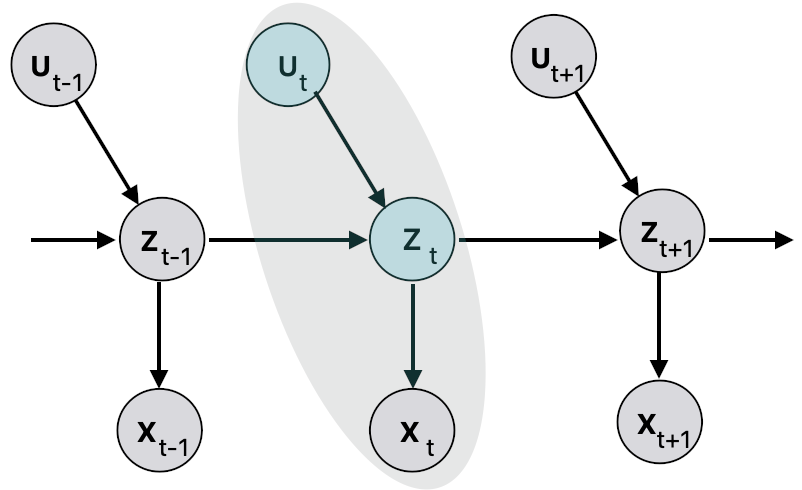
\includegraphics[width=200px]{./Images/dkf_model.png}
    \caption{DKF model as a Bayesian network. The inputs
    $\mathbf{u}_t$ are always observed.}
    \label{fig:dkf_model}
\end{figure}

\subsection{Generative model}\label{seq:generative_model}

The generative model is the joint distribution of observations and
latent states given the inputs,
$p(\mathbf{x}_{1:T}, \mathbf{z}_{1:T} \mid \mathbf{u}_{1:T})$. Ordering
the variables in time and applying the product rule,
\begin{align*}
    p(\mathbf{x}_{1:T}, \mathbf{z}_{1:T} \mid \mathbf{u}_{1:T})
    &= \prod_{t=1}^T p(\mathbf{x}_t, \mathbf{z}_t \mid \mathbf{x}_{1:t-1},
       \mathbf{z}_{1:t-1}, \mathbf{u}_{1:T}) \\
    &= \prod_{t=1}^T p(\mathbf{x}_t \mid \mathbf{x}_{1:t-1},
       \mathbf{z}_{1:t}, \mathbf{u}_{1:T})\,
       p(\mathbf{z}_t \mid \mathbf{x}_{1:t-1}, \mathbf{z}_{1:t-1},
       \mathbf{u}_{1:T}).
\end{align*}
The graph of Figure~\ref{fig:dkf_model} then simplifies each factor.
Using d-separation (Annex~\ref{seq:d_separation}):
\begin{itemize}
    \item $\mathbf{z}_{t} \indep (\mathbf{x}_{1:t-1},
    \mathbf{z}_{1:t-2}, \mathbf{u}_{1:t-1}, \mathbf{u}_{t+1:T}) \mid
    \mathbf{z}_{t-1}, \mathbf{u}_t$: every path from the past to
    $\mathbf{z}_t$ goes through $\mathbf{z}_{t-1}$, as a chain node or a
    fork node, and $\mathbf{z}_{t-1}$ is given. Future inputs only reach
    $\mathbf{z}_t$ through colliders on unobserved future states.
    \item $\mathbf{x}_{t} \indep (\mathbf{x}_{1:t-1}, \mathbf{z}_{1:t-1},
    \mathbf{u}_{1:T}) \mid \mathbf{z}_{t}$: $\mathbf{z}_t$ is the only
    parent of $\mathbf{x}_t$, and every path into $\mathbf{x}_t$ goes
    through it.
\end{itemize}
Hence\footnote{For $t=1$, $p(\mathbf{z}_t \mid \mathbf{z}_{t-1},
\mathbf{u}_{t})$ stands for $p(\mathbf{z}_1 \mid \mathbf{z}_0,
\mathbf{u}_{1})$, the prior on $\mathbf{z}_1$.}
\begin{equation}
    p(\mathbf{x}_{1:T}, \mathbf{z}_{1:T} \mid \mathbf{u}_{1:T}) =
    \prod_{t=1}^T p(\mathbf{x}_t \mid \mathbf{z}_{t})\,
    p(\mathbf{z}_t \mid \mathbf{z}_{t-1}, \mathbf{u}_{t}).
    \label{eq:generative_model}
\end{equation}

\section{The posterior and the inference model}\label{sec:posterior}

Learning a \emph{causal} generative model does not require \emph{causal}
inference. To infer $\mathbf{z}_t$ we may use all observations, past and
future, exactly as a Kalman smoother does.

\subsection{The four inference models of the paper}

Krishnan et al.\ \cite{krishnan2015deep} experiment with four
variational models:
\begin{itemize}
    \item \textbf{q-INDEP}: $q(\mathbf{z}_t \mid \mathbf{x}_t,
    \mathbf{u}_t)$, parameterised by a multi-layer perceptron (MLP);
    \item \textbf{q-LR}: $q(\mathbf{z}_t \mid \mathbf{x}_{t-1},
    \mathbf{x}_t, \mathbf{x}_{t+1}, \mathbf{u}_{t-1}, \mathbf{u}_t,
    \mathbf{u}_{t+1})$, parameterised by an MLP;
    \item \textbf{q-RNN}: $q(\mathbf{z}_t \mid \mathbf{x}_{1:t},
    \mathbf{u}_{1:t})$, parameterised by a recurrent neural network (RNN);
    \item \textbf{q-BRNN}: $q(\mathbf{z}_t \mid \mathbf{x}_{1:T},
    \mathbf{u}_{1:T})$, parameterised by a bidirectional RNN.
\end{itemize}
None of these conditions on the previous latent state: the latent
states are independent given the observations. Such \emph{mean-field}
approximations cannot represent the strong correlation between
successive states of the true posterior. The same paper, however, writes
the posterior in its structured form (its Equation~3), and the authors'
follow-up work \cite{krishnan2017structured} builds an inference network
of exactly that form, with a \enquote{combiner} that merges
$\mathbf{z}_{t-1}$ with an RNN summary of the observations. My
implementation follows the structured form, derived next.

\subsection{Structure of the true posterior}

By the product rule,
\[
    p_{\theta}(\mathbf{z}_{1:T} \mid \mathbf{x}_{1:T}, \mathbf{u}_{1:T})
    = \prod_{t=1}^T p_{\theta}(\mathbf{z}_t \mid \mathbf{z}_{1:t-1},
    \mathbf{x}_{1:T}, \mathbf{u}_{1:T}).
\]
Given $\mathbf{z}_{t-1}$, the past variables $\mathbf{z}_{1:t-2}$,
$\mathbf{x}_{1:t-1}$ and $\mathbf{u}_{1:t-1}$ are d-separated from
$\mathbf{z}_{t}$: in the graph, every path from them to $\mathbf{z}_t$
passes through $\mathbf{z}_{t-1}$ as a chain node or a fork node, and
observing $\mathbf{x}$ or $\mathbf{u}$ cannot open a path, because no
$\mathbf{x}$ or $\mathbf{u}$ node is a collider on such a path. The
future observations $\mathbf{x}_{t:T}$, on the other hand, remain
dependent on $\mathbf{z}_t$. Therefore
\begin{equation*}
    p_{\theta}(\mathbf{z}_{1:T} \mid \mathbf{x}_{1:T}, \mathbf{u}_{1:T})
    = \prod_{t=1}^T p_{\theta}\big(\mathbf{z}_t \mid
    \mathbf{z}_{t-1}, \mathbf{x}_{\textcolor{blue}{t}:T},
    \mathbf{u}_{\textcolor{blue}{t}:T}\big),
\end{equation*}
and it is natural to choose an inference model with the same structure:
\begin{equation}
    q_{\phi}(\mathbf{z}_{1:T} \mid \mathbf{x}_{1:T}, \mathbf{u}_{1:T}) =
    \prod_{t=1}^T q_{\phi}\big(\mathbf{z}_t \mid \mathbf{z}_{t-1},
    \mathbf{x}_{\textcolor{blue}{t}:T},
    \mathbf{u}_{\textcolor{blue}{t}:T}\big).
    \label{q_phi}
\end{equation}

\begin{inwords}
Once you know where the state was at time $t-1$, the past observations
have nothing more to tell you about the state at time $t$: their
information has been \enquote{absorbed} by $\mathbf{z}_{t-1}$. The
future observations, however, still matter, because they were generated
from states that $\mathbf{z}_t$ influences. So the posterior factor for
$\mathbf{z}_t$ needs exactly two ingredients: the previous state and a
summary of the observations from $t$ to $T$. The inference network is
built to receive exactly these two ingredients, and nothing else.
\end{inwords}

\begin{story}[{Notation for $t=1$}]
To keep formulas short, I write $p_{\theta}(\mathbf{z}_{t} \mid
\mathbf{z}_{t-1}, \star)$ and $q_{\phi}(\mathbf{z}_{t} \mid
\mathbf{z}_{t-1}, \star)$ also for $t = 1$, where $\mathbf{z}_0$ is the
fixed or learned initial value. Thus $p_{\theta}(\mathbf{z}_{1} \mid
\mathbf{z}_{0}, \star)$ is the prior on $\mathbf{z}_{1}$.
\end{story}

\section{Evidence Lower Bound}\label{sec:elbo}

The ELBO has the same definition as for the VAE, with the whole sequence
in place of a single data point:
\begin{align*}
    \mathcal{L}(\theta, \phi; \mathbf{x}_{1:T}, \mathbf{u}_{1:T}) =
    \E_{q_\phi(\mathbf{z}_{1:T} \mid \mathbf{x}_{1:T}, \mathbf{u}_{1:T})}
    \left[ \log \frac{p_\theta(\mathbf{x}_{1:T}, \mathbf{z}_{1:T} \mid
    \mathbf{u}_{1:T})}{q_\phi(\mathbf{z}_{1:T} \mid \mathbf{x}_{1:T},
    \mathbf{u}_{1:T})} \right]
    \;\leq\; \log p_\theta(\mathbf{x}_{1:T} \mid \mathbf{u}_{1:T}),
\end{align*}
and, as in \eqref{eq:elbo_gap}, the gap is
$\KL\big(q_\phi(\mathbf{z}_{1:T} \mid \mathbf{x}_{1:T}, \mathbf{u}_{1:T})
\,\|\, p_\theta(\mathbf{z}_{1:T} \mid \mathbf{x}_{1:T},
\mathbf{u}_{1:T})\big)$. Substituting the factorisations
\eqref{eq:generative_model} and \eqref{q_phi}, Appendix~\ref{sec:elbo_derivation}
shows that
\begin{equation}
\boxed{
\begin{aligned}
    \mathcal{L}(\theta, \phi) =\ &
    \sum_{t=1}^T \E_{q_{\phi}(\mathbf{z}_{t} \mid \mathbf{x}_{1:T},
    \mathbf{u}_{1:T})} \big[\log p_\theta(\mathbf{x}_t \mid
    \mathbf{z}_{t})\big] \\
    & - \sum_{t=1}^T \E_{q_\phi(\mathbf{z}_{t-1} \mid \mathbf{x}_{1:T},
    \mathbf{u}_{1:T})} \Big[ \KL\big( q_\phi(\mathbf{z}_t \mid
    \mathbf{z}_{t-1}, \mathbf{x}_{t:T}, \mathbf{u}_{t:T}) \,\big\|\,
    p_\theta(\mathbf{z}_t \mid \mathbf{z}_{t-1}, \mathbf{u}_{t}) \big)
    \Big]
\end{aligned}
}
\label{eq:dkf_elbo}
\end{equation}
where, for $t = 1$, the outer expectation is trivial because
$\mathbf{z}_0$ is fixed.
\begin{itemize}
    \item The \textbf{reconstruction term} measures how well each
    observation is explained by its latent state.
    \item The \textbf{regularisation term} measures, at each time step,
    how far the inference network's distribution for $\mathbf{z}_t$ is
    from what the dynamics predict from $\mathbf{z}_{t-1}$.
\end{itemize}

\begin{inwords}
The KL divergence between two distributions over whole trajectories
splits into one KL per time step: this is the \emph{chain rule} of the
KL divergence, and it holds because both the model and the inference
network are Markov chains. Each per-step KL compares two Gaussians for
$\mathbf{z}_t$ \emph{given} $\mathbf{z}_{t-1}$, so it has a closed form,
however complicated the neural networks are. The price is the outer
expectation over $\mathbf{z}_{t-1}$, which Section~\ref{sec:approximation_elbo}
shows how to handle.
\end{inwords}

\section{DKF Inference Model Design}

The datasets used in this project have no control input, so from now on
$\mathbf{u}$ is dropped:
\begin{equation*}
    q_{\phi}(\mathbf{z}_{1:T} \mid \mathbf{x}_{1:T}) =
    \prod_{t=1}^T q_{\phi}(\mathbf{z}_t \mid \mathbf{z}_{t-1},
    \mathbf{x}_{t:T}).
\end{equation*}
Each factor is a Gaussian with diagonal covariance,
\begin{equation*}
    q_{\phi}(\mathbf{z}_t \mid \mathbf{z}_{t-1}, \mathbf{x}_{t:T}) =
    \mathcal{N}\big(\mathbf{z}_t;\ \boldsymbol{\mu}_{\phi}(\mathbf{z}_{t-1},
    \mathbf{x}_{t:T}),\ \mathrm{diag}(\boldsymbol{\sigma}^2_{\phi}
    (\mathbf{z}_{t-1}, \mathbf{x}_{t:T}))\big),
\end{equation*}
whose parameters are computed by neural networks\footnote{The networks
output $\log \boldsymbol{\sigma}^2$ rather than $\boldsymbol{\sigma}^2$,
so that the variance, obtained with an exponential, is always
positive.}. The dependence on the whole suffix $\mathbf{x}_{t:T}$ is
handled by a \textbf{backward RNN} (an LSTM run from $T$ down to $1$,
Appendix~\ref{sec:backward_lstm}): its output at time $t$, written
$\mathbf{b}_t$, summarises $\mathbf{x}_{t:T}$
(Figure~\ref{fig:backward_rnn}). At each time step, a \textbf{combiner}
(Appendix~\ref{combiner_info}) merges $\mathbf{z}_{t-1}$ with
$\mathbf{b}_t$, and an MLP, the \textbf{encoder}, maps the result to
$\boldsymbol{\mu}_{\phi}$ and $\log \boldsymbol{\sigma}^2_{\phi}$.

\begin{figure}[ht!]
    \centering
    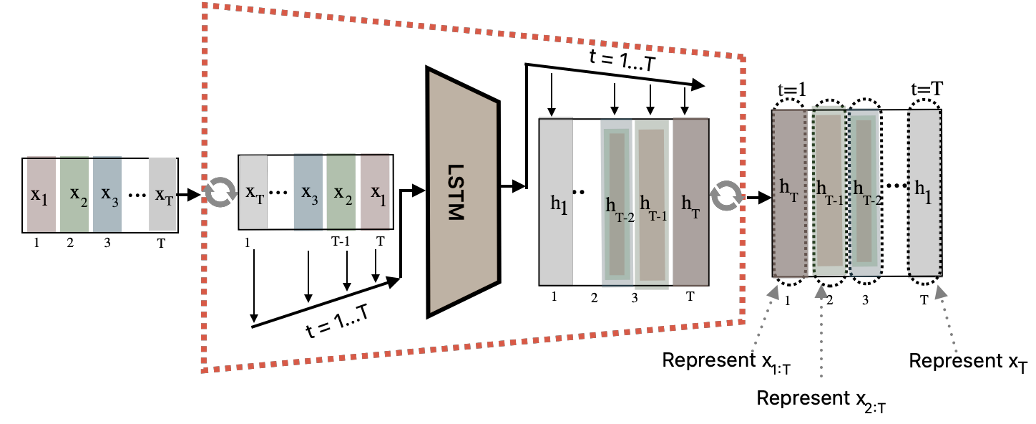
\includegraphics[width=400px]{./Images/backward_lstm.png}
    \caption{Backward RNN: the output at position $t$ summarises
    $\mathbf{x}_{t:T}$.}
    \label{fig:backward_rnn}
\end{figure}

\subsection{Reparameterisation trick}

As in the VAE, $\mathbf{z}_t$ is sampled as
\begin{equation*}
    \mathbf{z}_t = \boldsymbol{\mu}_{\phi}(\mathbf{z}_{t-1},
    \mathbf{x}_{t:T}) + \boldsymbol{\sigma}_{\phi}(\mathbf{z}_{t-1},
    \mathbf{x}_{t:T}) \odot \boldsymbol{\epsilon}_t,
    \qquad \boldsymbol{\epsilon}_t \sim \mathcal{N}(\mathbf{0},
    \mathbf{I}),
\end{equation*}
with $\boldsymbol{\sigma}_{\phi}$ the vector of standard deviations.
Note that $\mathbf{z}_{t-1}$ is itself a sample, so $\mathbf{z}_t$ is a
differentiable function of $\phi$ and of all the noises
$\boldsymbol{\epsilon}_1, \dots, \boldsymbol{\epsilon}_t$.

\subsection{Overall design}

The whole inference model is shown in Figure~\ref{fig:dkf_inference}.

\begin{figure}[ht!]
    \centering
    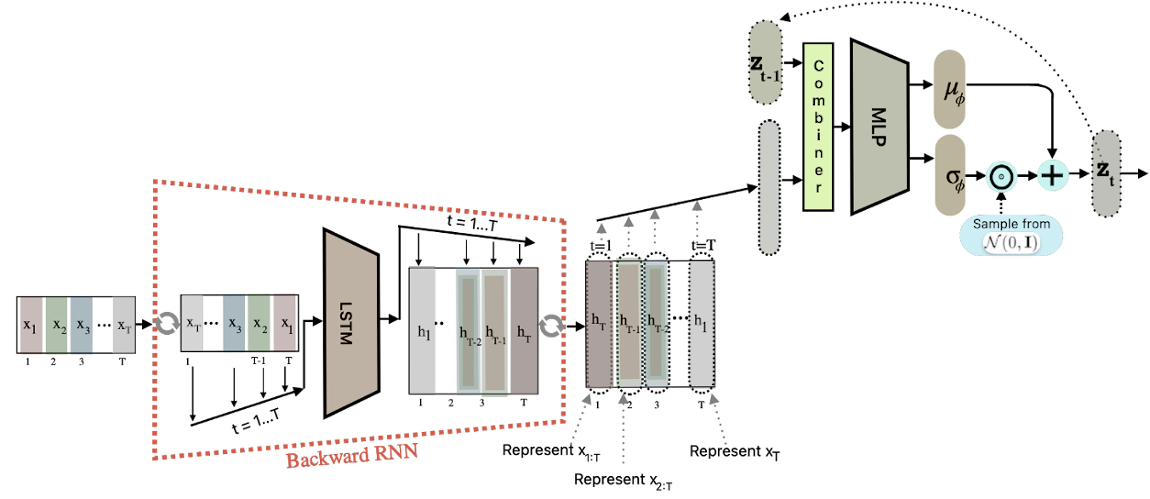
\includegraphics[width=450px]{./Images/dkf_detailed_inference.png}
    \caption{DKF inference model}
    \label{fig:dkf_inference}
\end{figure}

\section{DKF Generative Model Design}

Without control input, the generative model \eqref{eq:generative_model}
reads
\begin{equation}
    p_{\theta}(\mathbf{x}_{1:T}, \mathbf{z}_{1:T}) =
    \prod_{t=1}^T p_{\theta_{\mathbf{x}}}(\mathbf{x}_t \mid \mathbf{z}_{t})
    \,p_{\theta_{\mathbf{z}}}(\mathbf{z}_t \mid \mathbf{z}_{t-1}),
    \label{eq:recall_generative_model}
\end{equation}
with diagonal Gaussians for both factors.

\paragraph{Transition model.}
\begin{equation*}
    p_{\theta_{\mathbf{z}}}(\mathbf{z}_t \mid \mathbf{z}_{t-1}) =
    \mathcal{N}\big(\mathbf{z}_t;\ \boldsymbol{\mu}_{\theta_{\mathbf{z}}}
    (\mathbf{z}_{t-1}),\ \mathrm{diag}(\boldsymbol{\sigma}^2_{
    \theta_{\mathbf{z}}}(\mathbf{z}_{t-1}))\big).
\end{equation*}

\paragraph{Emission (reconstruction) model.}
\begin{equation*}
    p_{\theta_{\mathbf{x}}}(\mathbf{x}_t \mid \mathbf{z}_{t}) =
    \mathcal{N}\big(\mathbf{x}_t;\ \boldsymbol{\mu}_{\theta_{\mathbf{x}}}
    (\mathbf{z}_{t}),\ \mathrm{diag}(\boldsymbol{\sigma}^2_{
    \theta_{\mathbf{x}}}(\mathbf{z}_{t}))\big).
\end{equation*}

Both pairs of parameters are computed by MLPs
(Figure~\ref{fig:dkf_generative}), which again output
$\log\boldsymbol{\sigma}^2$.

\begin{figure}[ht!]
    \centering
    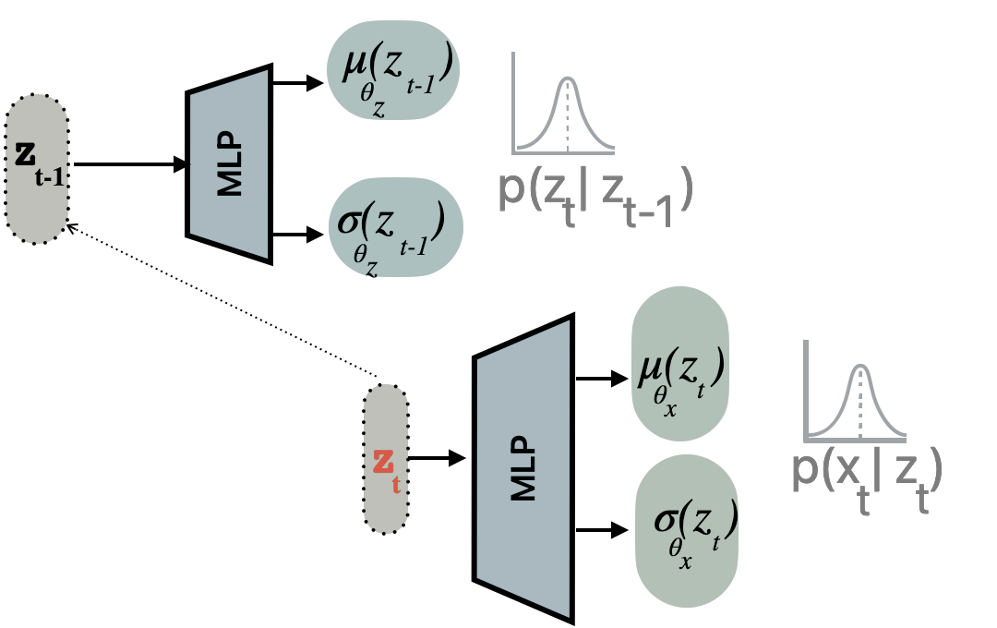
\includegraphics[width=250px]{./Images/dkf_generative.png}
    \caption{DKF generative model}
    \label{fig:dkf_generative}
\end{figure}

\begin{story}[Reconstruction]
Given a latent state $\mathbf{z}_t$, the most likely observation is the
mean $\hat{\mathbf{x}}_{t} = \boldsymbol{\mu}_{\theta_{\mathbf{x}}}
(\mathbf{z}_{t})$. This is what I call the \enquote{reconstruction} of
$\mathbf{x}_t$ in the experiments.
\end{story}

%~~~~~~~~~~~~~~~~~~~~~~~~~~~~~~~~~~~~~~~~~~~~~~~~~~~~~~~~~~~~~~~~~~~~~~~~
\section{Estimating the ELBO}\label{sec:approximation_elbo}

\subsection{The difficulty}

Both terms of \eqref{eq:dkf_elbo} are expectations under
\emph{marginals} of the inference model,
$q_\phi(\mathbf{z}_{t} \mid \mathbf{x}_{1:T})$ and
$q_\phi(\mathbf{z}_{t-1} \mid \mathbf{x}_{1:T})$. These marginals are
intractable: for instance
\[
    q_\phi(\mathbf{z}_{t} \mid \mathbf{x}_{1:T}) = \int
    q_\phi(\mathbf{z}_{t} \mid \mathbf{z}_{t-1}, \mathbf{x}_{t:T})\,
    q_\phi(\mathbf{z}_{t-1} \mid \mathbf{x}_{1:T})\,d\mathbf{z}_{t-1}
\]
is an integral over all the earlier latent states. With non-linear
networks it is not Gaussian, and in general it has no closed form at all.

\subsection{Ancestral sampling}

We never need the \emph{density} of these marginals, only
\emph{samples} from them. Draw one trajectory by ancestral sampling:
\begin{equation*}
    \dot{\mathbf{z}}_1 \sim q_\phi(\mathbf{z}_1 \mid \mathbf{z}_0,
    \mathbf{x}_{1:T}),\quad
    \dot{\mathbf{z}}_2 \sim q_\phi(\mathbf{z}_2 \mid \dot{\mathbf{z}}_1,
    \mathbf{x}_{2:T}),\quad \dots,\quad
    \dot{\mathbf{z}}_T \sim q_\phi(\mathbf{z}_T \mid
    \dot{\mathbf{z}}_{T-1}, \mathbf{x}_{T}).
\end{equation*}
By \eqref{q_phi}, the trajectory $\dot{\mathbf{z}}_{1:T}$ is an exact
sample from the joint $q_\phi(\mathbf{z}_{1:T} \mid \mathbf{x}_{1:T})$.
Consequently, each $\dot{\mathbf{z}}_t$ is an exact sample from the
marginal $q_\phi(\mathbf{z}_{t} \mid \mathbf{x}_{1:T})$. One trajectory
provides samples of every marginal at once.

\subsection{The estimator}

Evaluate both terms of \eqref{eq:dkf_elbo} along the sampled trajectory:
\begin{equation}
    \hat{\mathcal{L}} = \sum_{t=1}^T \log p_\theta(\mathbf{x}_t \mid
    \dot{\mathbf{z}}_t) - \sum_{t=1}^T \KL\big(q_\phi(\mathbf{z}_t \mid
    \dot{\mathbf{z}}_{t-1}, \mathbf{x}_{t:T}) \,\big\|\,
    p_\theta(\mathbf{z}_t \mid \dot{\mathbf{z}}_{t-1})\big),
    \label{eq:elbo_estimator}
\end{equation}
where each KL is computed in closed form
(Appendix~\ref{sec:elbo_regularization}) at the sampled
$\dot{\mathbf{z}}_{t-1}$.

\begin{proposition}\label{prop:unbiased}
$\E\big[\hat{\mathcal{L}}\big] = \mathcal{L}(\theta, \phi;
\mathbf{x}_{1:T})$: the single-trajectory estimator is unbiased.
\end{proposition}
\begin{proof}
By linearity of expectation it is enough to treat each term. Since
$\dot{\mathbf{z}}_t \sim q_\phi(\mathbf{z}_{t} \mid \mathbf{x}_{1:T})$,
$\E[\log p_\theta(\mathbf{x}_t \mid \dot{\mathbf{z}}_t)] =
\E_{q_\phi(\mathbf{z}_{t} \mid \mathbf{x}_{1:T})}[\log
p_\theta(\mathbf{x}_t \mid \mathbf{z}_t)]$. Likewise, since
$\dot{\mathbf{z}}_{t-1} \sim q_\phi(\mathbf{z}_{t-1} \mid
\mathbf{x}_{1:T})$, the expectation of the $t$-th KL term is the
expectation of the KL under $q_\phi(\mathbf{z}_{t-1} \mid
\mathbf{x}_{1:T})$. These are exactly the terms of \eqref{eq:dkf_elbo}.
\end{proof}

\begin{inwords}
Each term of the ELBO is an average of something over the latent states.
Averages can be estimated by plugging in samples, and nothing non-linear
is applied to those averages afterwards. So one sampled trajectory gives
an estimate that is right on average: some trajectories overshoot, some
undershoot, and the errors cancel in expectation. That is what makes
training with one trajectory per sequence legitimate. Averaging over the
sequences of a minibatch then reduces the noise.
\end{inwords}

A numerical demonstration of Proposition~\ref{prop:unbiased}, on a
model where the ELBO can be computed exactly, is in the notebook
\href{https://github.com/CL-BZH/Deep-Kalman-Filters/blob/main/Notebooks/elbo_expectations.ipynb}{\texttt{elbo\_expectations.ipynb}}.

\subsection{Why compute the KL terms in closed form?}

One could also estimate the regularisation term by sampling, using
$\log q_\phi(\dot{\mathbf{z}}_t \mid \dot{\mathbf{z}}_{t-1},
\mathbf{x}_{t:T}) - \log p_\theta(\dot{\mathbf{z}}_t \mid
\dot{\mathbf{z}}_{t-1})$ in place of each KL. That is also unbiased.
Computing the KL in closed form instead integrates $\mathbf{z}_t$ out
exactly given $\dot{\mathbf{z}}_{t-1}$. This is
\emph{Rao--Blackwellisation}, and by the law of total variance it lowers
the variance of each KL term. Krishnan et al.\ report that sampling the
KL term gives high-variance gradients, which motivates this choice.

Two remarks are worth making. First, the factorisation
\eqref{eq:dkf_elbo} is what makes a closed form possible at all: the KL
between two distributions over whole trajectories has no closed form
when the transition is a neural network, while each per-step KL is
between two diagonal Gaussians. Second, lower variance for each term
does not guarantee lower variance for the whole estimate, because the
sampled terms are correlated. In the experiments of the notebook cited
above, the closed-form KL gave less noisy gradients for every encoder
tried, but the sampled version gave a less noisy \emph{value} of the
ELBO when the encoder was close to the true posterior.

\subsection{Differentiability}

With the reparameterisation trick, $\hat{\mathcal{L}}$ is a
differentiable function of $\theta$ and $\phi$ for fixed noises
$\boldsymbol{\epsilon}_{1:T}$, and its gradient is an unbiased estimate
of $\nabla\mathcal{L}$. This is all stochastic gradient descent needs.

%~~~~~~~~~~~~~~~~~~~~~~~~~~~~~~~~~~~~~~~~~~~~~~~~~~~~~~~~~~~~~~~~~~~~~~~~
\section{Training the DKF}\label{sec:training}

The DKF is trained by minimising $-\hat{\mathcal{L}}$, averaged over a
minibatch of sequences, with respect to $\theta_{\mathbf{x}}$,
$\theta_{\mathbf{z}}$ and $\phi$, using the Adam optimiser. The complete
model is shown in Figure~\ref{fig:dkf}.

\begin{figure}[ht!]
    \centering
    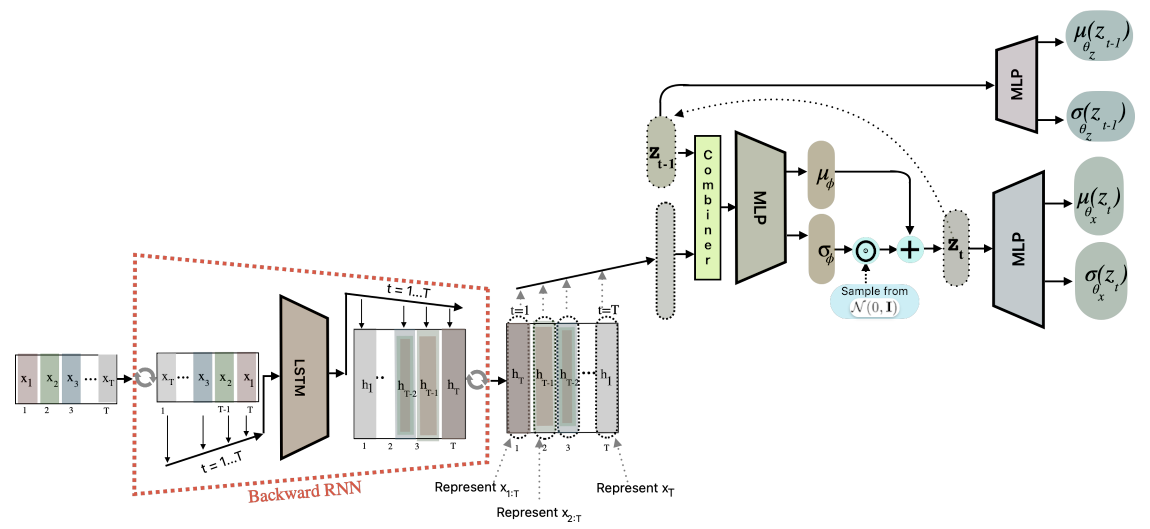
\includegraphics[width=460px]{./Images/dkf.png}
    \caption{DKF model: inference network (left and centre) and
    generative networks (right).}
    \label{fig:dkf}
\end{figure}

\subsection*{One training step}

\begin{enumerate}
    \item \textbf{Summarise the future.} Run the backward RNN over
    $\mathbf{x}_{1:T}$ to obtain $\mathbf{b}_1, \dots, \mathbf{b}_T$,
    where $\mathbf{b}_t$ summarises $\mathbf{x}_{t:T}$.

    \item \textbf{Sample a latent trajectory (ancestral sampling).} For
    $t = 1, \dots, T$: combine $\dot{\mathbf{z}}_{t-1}$ with
    $\mathbf{b}_t$, compute $\boldsymbol{\mu}_{\phi}$ and
    $\log\boldsymbol{\sigma}^2_{\phi}$ with the encoder, and draw
    $\dot{\mathbf{z}}_t$ with the reparameterisation trick.

    \item \textbf{Evaluate the transition.} For each $t$, compute
    $\boldsymbol{\mu}_{\theta_{\mathbf{z}}}(\dot{\mathbf{z}}_{t-1})$ and
    $\log\boldsymbol{\sigma}^2_{\theta_{\mathbf{z}}}
    (\dot{\mathbf{z}}_{t-1})$ at the \emph{sampled} previous state.

    \item \textbf{Decode.} For each $t$, compute
    $\boldsymbol{\mu}_{\theta_{\mathbf{x}}}(\dot{\mathbf{z}}_{t})$ and
    $\log\boldsymbol{\sigma}^2_{\theta_{\mathbf{x}}}(\dot{\mathbf{z}}_{t})$.

    \item \textbf{Compute the loss} $-\hat{\mathcal{L}}$
    (Section~\ref{sec:loss}).

    \item \textbf{Update.} Backpropagate through the whole computation,
    including the sampling steps thanks to the reparameterisation trick,
    and take one optimiser step.
\end{enumerate}

\subsection{The loss function}\label{sec:loss}

Using \eqref{eq:sum_log_p_theta_x_given_z} (Appendix~\ref{sec:elbo_recon})
and \eqref{eq:regularization_term}
(Appendix~\ref{sec:elbo_regularization}), and writing $d_x$ and $d_z$ for
the dimensions of $\mathbf{x}_t$ and $\mathbf{z}_t$,
\begin{align*}
    -\sum_{t=1}^T \log p_{\theta_{\mathbf{x}}}(\mathbf{x}_t \mid
    \dot{\mathbf{z}}_{t}) &= \frac{T d_x}{2} \log(2\pi) +
    \frac{1}{2} \sum_{t=1}^T \sum_{i=1}^{d_x} \left[ \log
    \sigma^2_{\theta_{\mathbf{x}}, i}(\dot{\mathbf{z}}_{t}) +
    \frac{\big(x_{t,i} - \mu_{\theta_{\mathbf{x}}, i}(\dot{\mathbf{z}}_{t})
    \big)^2}{\sigma^2_{\theta_{\mathbf{x}}, i}(\dot{\mathbf{z}}_{t})}
    \right], \\
    \sum_{t=1}^T \KL_t &= -\frac{T d_z}{2} + \frac{1}{2} \sum_{t=1}^T
    \sum_{i=1}^{d_z} \left[ \frac{\sigma^2_{\phi, i} + (\mu_{\theta_{
    \mathbf{z}}, i} - \mu_{\phi, i})^2}{\sigma^2_{\theta_{\mathbf{z}},
    i}} + \log \sigma^2_{\theta_{\mathbf{z}}, i} - \log \sigma^2_{\phi,
    i} \right],
\end{align*}
where, in the second line, the parameters of $q_\phi$ are evaluated at
$(\dot{\mathbf{z}}_{t-1}, \mathbf{x}_{t:T})$ and those of
$p_{\theta_{\mathbf{z}}}$ at $\dot{\mathbf{z}}_{t-1}$. The constants
$\frac{T d_x}{2}\log(2\pi)$ and $-\frac{T d_z}{2}$ do not depend on the
parameters and can be dropped. This leaves the two losses

\begin{center}
\boxed{
    \mathcal{L}_{\text{rec}} = \frac{1}{2} \sum_{t=1}^T
    \sum_{i=1}^{d_x} \left[ \log \sigma^2_{\theta_{\mathbf{x}}, i} +
    \frac{(x_{t,i} - \mu_{\theta_{\mathbf{x}}, i})^2}
    {\sigma^2_{\theta_{\mathbf{x}}, i}} \right]
}
\qquad
\boxed{
    \mathcal{L}_{\text{reg}} = \frac{1}{2} \sum_{t=1}^T
    \sum_{i=1}^{d_z} \left[ \frac{\sigma^2_{\phi, i} +
    (\mu_{\theta_{\mathbf{z}}, i} - \mu_{\phi, i})^2}
    {\sigma^2_{\theta_{\mathbf{z}}, i}} + \log
    \sigma^2_{\theta_{\mathbf{z}}, i} - \log \sigma^2_{\phi, i}
    \right]
}
\end{center}
and $-\hat{\mathcal{L}} = \mathcal{L}_{\text{rec}} +
\mathcal{L}_{\text{reg}} + \text{const}$.

\begin{story}[What the code computes]
The function \code{loss\_function} in \code{Utils/loss\_fcts.py}
computes $\frac{2}{T}\big(\mathcal{L}_{\text{rec}} + \beta\,
\mathcal{L}_{\text{reg}}\big)$, averaged over the minibatch: the factor
$\frac12$ is omitted and the result is divided by the sequence length.
Neither changes the minimiser. With $\beta = 1$ this is exactly the
negative ELBO estimate \eqref{eq:elbo_estimator}, up to a constant and a
positive factor. With $\beta \neq 1$ the objective is a weighted
($\beta$-VAE-style) variant. The option \code{loss\_type='mse'} drops the
decoder variance, so its reconstruction term is no longer a
log-likelihood and the objective is no longer an ELBO.
\end{story}

%~~~~~~~~~~~~~~~~~~~~~~~~~~~~~~~~~~~~~~~~~~~~~~~~~~~~~~~~~~~~~~~~~~~~~~~~
\section{Implementation}

The main classes of the implementation\footnote{The code is available
\href{https://github.com/CL-BZH/Deep-Kalman-Filters/tree/main}{on
GitHub}.} are shown in Figure~\ref{fig:dkf_implementation_objects}.

\begin{figure}[ht!]
    \centering
    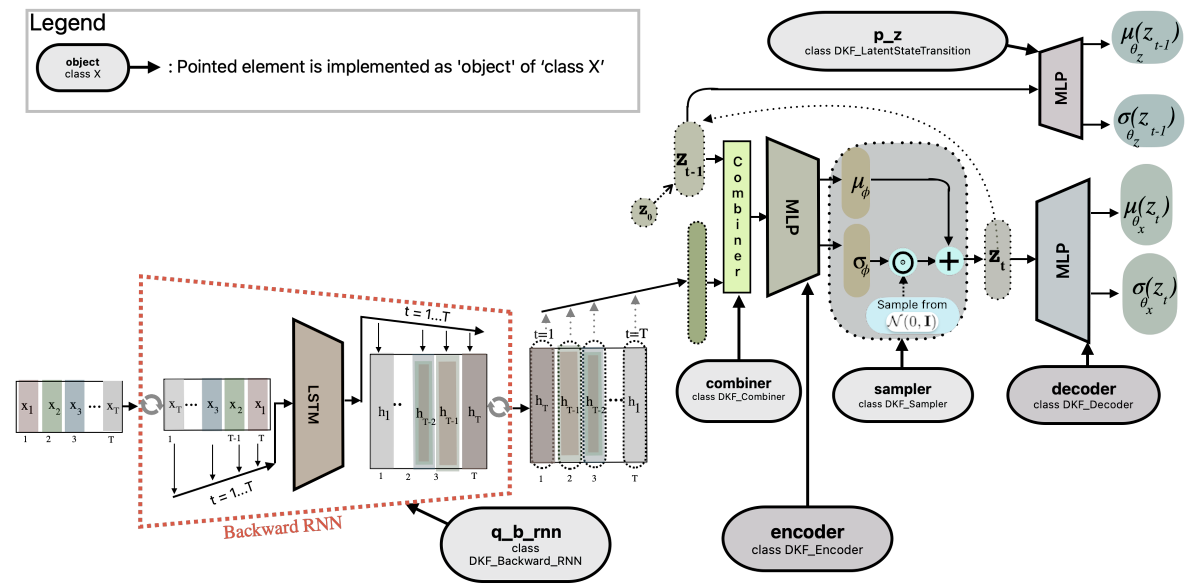
\includegraphics[width=460px]{./Images/dkf_implementation_objects.png}
    \caption{DKF implementation classes}
    \label{fig:dkf_implementation_objects}
\end{figure}

\subsection{The forward pass}

The \code{forward} method of the \code{DKF} class implements steps 1 to
4 of the training procedure for a minibatch of sequences
$\mathbf{x}$ of shape \code{(seq\_len, batch\_size, x\_dim)}.
\begin{enumerate}
    \item \textbf{Initial state.} $\mathbf{z}_0$ is the learnable
    parameter \code{Z\_0} if \code{learnable\_init\_z=True}, and a tensor
    of zeros otherwise. It is expanded to the batch size.
    \item \textbf{Backward RNN.} $\mathbf{x}$ is passed through the
    backward RNN \code{q\_b\_rnn}, which returns
    $\mathbf{b}_1, \dots, \mathbf{b}_T$.
    \item \textbf{Ancestral sampling.} For each $t$, the \code{combiner}
    merges the previous sample with $\mathbf{b}_t$, the \code{encoder}
    returns $\boldsymbol{\mu}_{\phi}$ and $\log\boldsymbol{\sigma}^2_{\phi}$,
    and the \code{sampler} draws $\dot{\mathbf{z}}_t$ with the
    reparameterisation trick. Means, log-variances and samples are
    stored.
    \item \textbf{Transition.} The transition network \code{p\_z} is
    applied to the shifted sequence
    $(\mathbf{z}_0, \dot{\mathbf{z}}_1, \dots, \dot{\mathbf{z}}_{T-1})$,
    giving the parameters of $p(\mathbf{z}_t \mid
    \dot{\mathbf{z}}_{t-1})$ for every $t$.
    \item \textbf{Decoding.} The \code{decoder} is applied to
    $\dot{\mathbf{z}}_{1:T}$ and returns
    $\hat{\mathbf{x}} = \boldsymbol{\mu}_{\theta_{\mathbf{x}}}$ and
    $\log\boldsymbol{\sigma}^2_{\theta_{\mathbf{x}}}$.
\end{enumerate}
It returns everything the loss function needs.

\subsection{The \texttt{predict} function}

\code{predict} takes an observed sequence $\mathbf{x}_{1:T}$ and returns
its reconstruction followed by \code{num\_steps} forecasts.
\begin{enumerate}
    \item It samples a latent trajectory $\dot{\mathbf{z}}_{1:T}$ exactly
    as in the forward pass, and decodes it to obtain the
    reconstruction.
    \item Starting from $\dot{\mathbf{z}}_T$, it repeatedly applies the
    transition model: it computes the parameters of
    $p(\mathbf{z}_{s} \mid \mathbf{z}_{s-1})$, samples
    $\mathbf{z}_{s}$, and decodes it into the forecast
    $\boldsymbol{\mu}_{\theta_{\mathbf{x}}}(\mathbf{z}_s)$.
\end{enumerate}

\begin{inwords}[Why this is the right way to forecast]
At the last time step, the inference network conditions only on
$\mathbf{z}_{T-1}$ and $\mathbf{x}_{T}$, so
$q_\phi(\mathbf{z}_T \mid \mathbf{x}_{1:T})$ approximates the
\emph{filtering} distribution $p(\mathbf{z}_T \mid \mathbf{x}_{1:T})$:
everything that has been observed, nothing more. Propagating samples of
it through the learned dynamics is the non-linear analogue of the Kalman
prediction step. Two limitations follow. A forecast is a single sampled
path, not the mean of the predictive distribution, so its error includes
the sampling noise. And the model can only forecast well if the
transition network has learned the dynamics. A very flexible inference
network can explain the training data while the transition network
stays poor (Appendix~\ref{sec:results}).
\end{inwords}

%======================================================================
\section{The Autoregressive DKF (AR DKF)}\label{sec:ar_dkf}

\subsection{Motivation}

On the sine-wave data, the vanilla DKF reconstructs the observed part of
a sequence well but fails to forecast it (Appendix~\ref{sec:results}).
Its forecasts depend only on the transition model
$p(\mathbf{z}_t \mid \mathbf{z}_{t-1})$, and nothing forces that model to
carry the information needed for long-range prediction. To give the
dynamics direct access to the history, I designed the
\enquote{Autoregressive} DKF (AR DKF), whose transition also depends on
the past observations:
\begin{equation*}
    p_{\theta_{\mathbf{z}}}(\mathbf{z}_t \mid \mathbf{z}_{t-1},
    \mathbf{x}_{0:t-1}),
\end{equation*}
where $\mathbf{x}_0$ is a fixed (zero) or learned initial value, so that
the transition into $\mathbf{z}_1$ is defined. In other words, the
independence $\mathbf{z}_t \indep \mathbf{x}_{1:t-1} \mid
\mathbf{z}_{t-1}$ of the vanilla DKF is given up on purpose by adding
edges from the past observations to $\mathbf{z}_t$
(Figure~\ref{fig:ar_dkf_transition_versus_dkf_transition}).

\begin{figure}[ht!]
    \centering
    \begin{minipage}{0.30\textwidth}
        \centering
        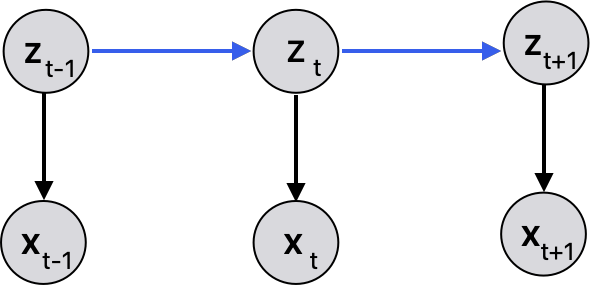
\includegraphics[width=1\textwidth]{./Images/dkf_transition_model.png}
        \subcaption{DKF model}
        \label{fig:dkf_transition_model}
    \end{minipage}
    \hspace{2cm}
    \begin{minipage}{0.30\textwidth}
        \centering
        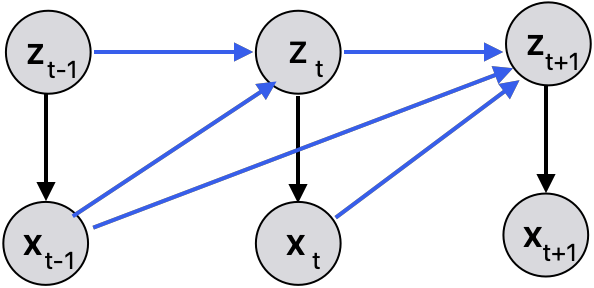
\includegraphics[width=1\textwidth]{./Images/ar_dkf_transition_model.png}
        \subcaption{AR DKF model}
        \label{fig:ar_dkf_transition_model}
    \end{minipage}
    \caption{DKF model versus AR DKF model (blue: the added edges).}
    \label{fig:ar_dkf_transition_versus_dkf_transition}
\end{figure}

\subsection{Generative model}

The joint distribution becomes
\begin{equation}
    p_{\theta}(\mathbf{x}_{1:T}, \mathbf{z}_{1:T}) =
    \prod_{t=1}^T p_{\theta_{\mathbf{x}}}(\mathbf{x}_t \mid \mathbf{z}_{t})
    \,p_{\theta_{\mathbf{z}}}(\mathbf{z}_t \mid \mathbf{z}_{t-1},
    \mathbf{x}_{0:t-1}).
    \label{eq:ar_generative}
\end{equation}
It is still a valid, causal generative model: each variable depends only
on variables generated before it. The history $\mathbf{x}_{0:t-1}$ is
summarised by a \textbf{forward RNN} (\code{pz\_f\_rnn}) run on the
shifted sequence $(\mathbf{x}_0, \mathbf{x}_1, \dots, \mathbf{x}_{T-1})$:
its output $\mathbf{h}_{t-1}$ summarises $\mathbf{x}_{0:t-1}$, and an MLP
maps $(\mathbf{z}_{t-1}, \mathbf{h}_{t-1})$ to the mean and log-variance
of the transition. The ELBO keeps the form \eqref{eq:dkf_elbo}, with
$p_{\theta_{\mathbf{z}}}(\mathbf{z}_t \mid \mathbf{z}_{t-1},
\mathbf{x}_{0:t-1})$ in the KL terms, and it is estimated in the same
way.

\subsection{What the new edges change for inference}\label{sec:ar_posterior}

Changing the generative model changes its posterior, and therefore the
inference network it needs. Redo the d-separation argument of
Section~\ref{sec:posterior} on the AR DKF graph.

\begin{proposition}\label{prop:ar_posterior}
In the AR DKF,
\begin{equation*}
    p_\theta(\mathbf{z}_{1:T} \mid \mathbf{x}_{1:T}) =
    \prod_{t=1}^T p_\theta(\mathbf{z}_t \mid \mathbf{z}_{t-1},
    \mathbf{x}_{\textcolor{red}{1}:T}),
\end{equation*}
and in general $p_\theta(\mathbf{z}_t \mid \mathbf{z}_{t-1},
\mathbf{x}_{1:T})$ depends on the past observations
$\mathbf{x}_{1:t-1}$ as well as on $\mathbf{x}_{t:T}$.
\end{proposition}
\begin{proof}
\emph{Earlier states drop out.} Take a path from $\mathbf{z}_s$, $s
\leq t-2$, to $\mathbf{z}_t$. Paths through the latent chain pass
through $\mathbf{z}_{t-1}$ as a chain or fork node and are blocked
because $\mathbf{z}_{t-1}$ is given. Any other path must pass through an
observation $\mathbf{x}_r$. Each observation has a single parent,
$\mathbf{z}_r$, so it can never be a collider on a path: the path passes
through $\mathbf{x}_r$ as a chain node ($\mathbf{z}_r \to \mathbf{x}_r
\to \mathbf{z}_{r'}$) or as a fork node ($\mathbf{z}_{r'} \leftarrow
\mathbf{x}_r \to \mathbf{z}_{r''}$). Since all observations are given,
such a path is blocked too.
\emph{Past observations do not drop out.} For $t \geq 2$,
$\mathbf{x}_{t-1}$ is a \emph{parent} of $\mathbf{z}_t$: the edge
$\mathbf{x}_{t-1} \to \mathbf{z}_t$ is a path of length one, with no
intermediate node that could block it. Hence no conditioning set can
make $\mathbf{z}_t$ independent of $\mathbf{x}_{t-1}$.
\end{proof}

\begin{inwords}
In the vanilla DKF, the past observations only influence $\mathbf{z}_t$
\emph{through} $\mathbf{z}_{t-1}$, so knowing $\mathbf{z}_{t-1}$ makes
them redundant. In the AR DKF they influence $\mathbf{z}_t$
\emph{directly}, through the new edges, so they can never become
redundant. The inference network for $\mathbf{z}_t$ must therefore see
the past observations as well as the future ones.
\end{inwords}

The AR DKF as implemented keeps the inference network of the vanilla
DKF, $q_\phi(\mathbf{z}_t \mid \mathbf{z}_{t-1}, \mathbf{x}_{t:T})$,
which ignores $\mathbf{x}_{1:t-1}$. By Proposition~\ref{prop:ar_posterior}
it cannot represent the true posterior, even with unlimited capacity, so
the gap $\KL(q_\phi \,\|\, p_\theta(\cdot \mid \mathbf{x}))$ in the ELBO
can never close. The variants of the next section repair this.

\subsection{Prediction}

Forecasting works as for the DKF, except that each transition step also
needs the summary $\mathbf{h}$ of the observations so far. After a
forecast $\hat{\mathbf{x}}_s$ is produced, it is appended to the
sequence and the forward RNN is run again, so that the next transition
step is conditioned on the model's own past forecasts. This makes the
AR DKF a genuinely autoregressive forecaster.

\begin{story}[A detail of the implementation]
In \code{predict}, the sequence fed to the forward RNN is a sliding
window: each new forecast is appended and the oldest observation is
removed, and the RNN is re-run from the start of the window. During
training, the RNN always starts from $\mathbf{x}_0$. The summaries seen
at prediction time are therefore computed slightly differently from
those seen during training.
\end{story}

The AR DKF design is shown in
Figure~\ref{fig:ar_dkf_implementation_objects}.

\begin{figure}[ht!]
    \centering
    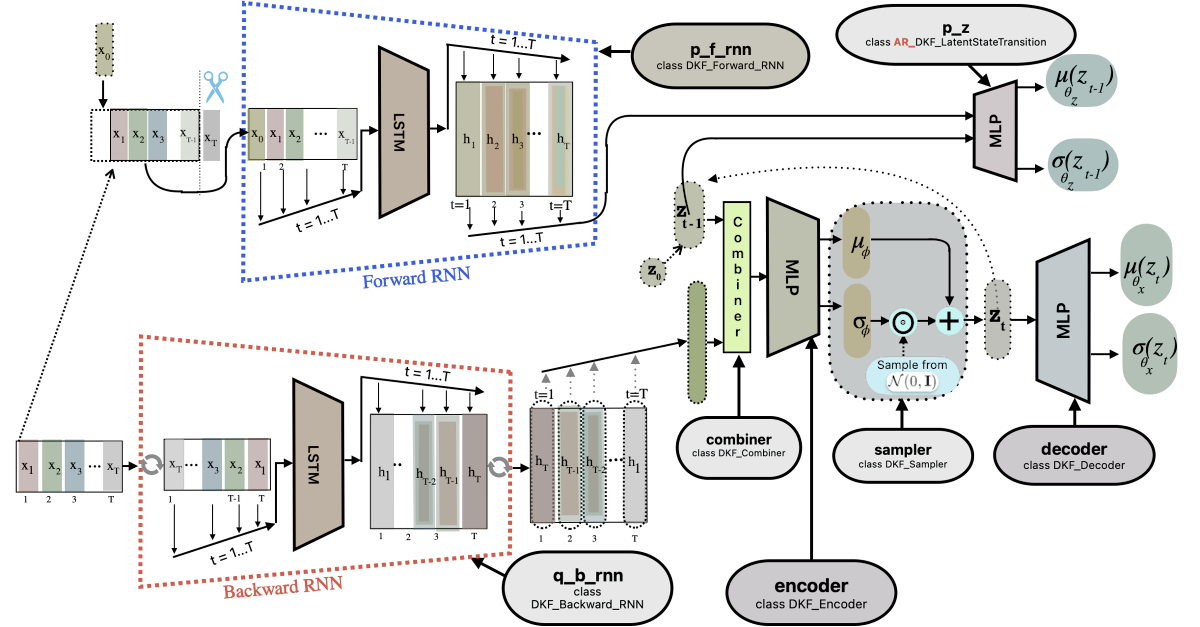
\includegraphics[width=480px]{./Images/ar_dkf_implementation_objects.png}
    \caption{AR DKF model}
    \label{fig:ar_dkf_implementation_objects}
\end{figure}

%- - - - - - - - - - - - - - - - - - - - - - - - - - - - - - - - - - - -
\section{The FAR DKF and BAR DKF models}\label{sec:far_bar}

The FAR DKF (\enquote{Forward Autoregressive}) and the BAR DKF
(\enquote{Bidirectional Autoregressive}) keep the generative model of the
AR DKF, including its transition $p_{\theta_{\mathbf{z}}}(\mathbf{z}_t
\mid \mathbf{z}_{t-1}, \mathbf{x}_{0:t-1})$, unchanged. They differ from it
only in the \textbf{inference network}, which in both variants receives
information about the past observations. By
Proposition~\ref{prop:ar_posterior}, this is exactly what the AR DKF
posterior requires.

\subsection{Forward Autoregressive DKF (FAR DKF)}

The FAR DKF adds a second forward RNN, \code{q\_f\_rnn}, to the inference
network (Figure~\ref{fig:far_dkf_implementation_objects}). Its output at
time $t$, $\overrightarrow{\mathbf{h}}_t$, summarises $\mathbf{x}_{1:t}$. The combiner
merges $\dot{\mathbf{z}}_{t-1}$ with both $\mathbf{b}_t$ (the future)
and $\overrightarrow{\mathbf{h}}_t$ (the past), so the inference model becomes
\begin{equation*}
    q_\phi(\mathbf{z}_t \mid \mathbf{z}_{t-1}, \mathbf{x}_{1:T}),
\end{equation*}
which has the structure of the true posterior of
Proposition~\ref{prop:ar_posterior}. The FAR DKF is therefore the
principled inference model for the AR DKF generative model. The linear
combiner offers separate weights for the two RNN summaries
(Appendix~\ref{combiner_info}).

\begin{figure}[ht!]
    \centering
    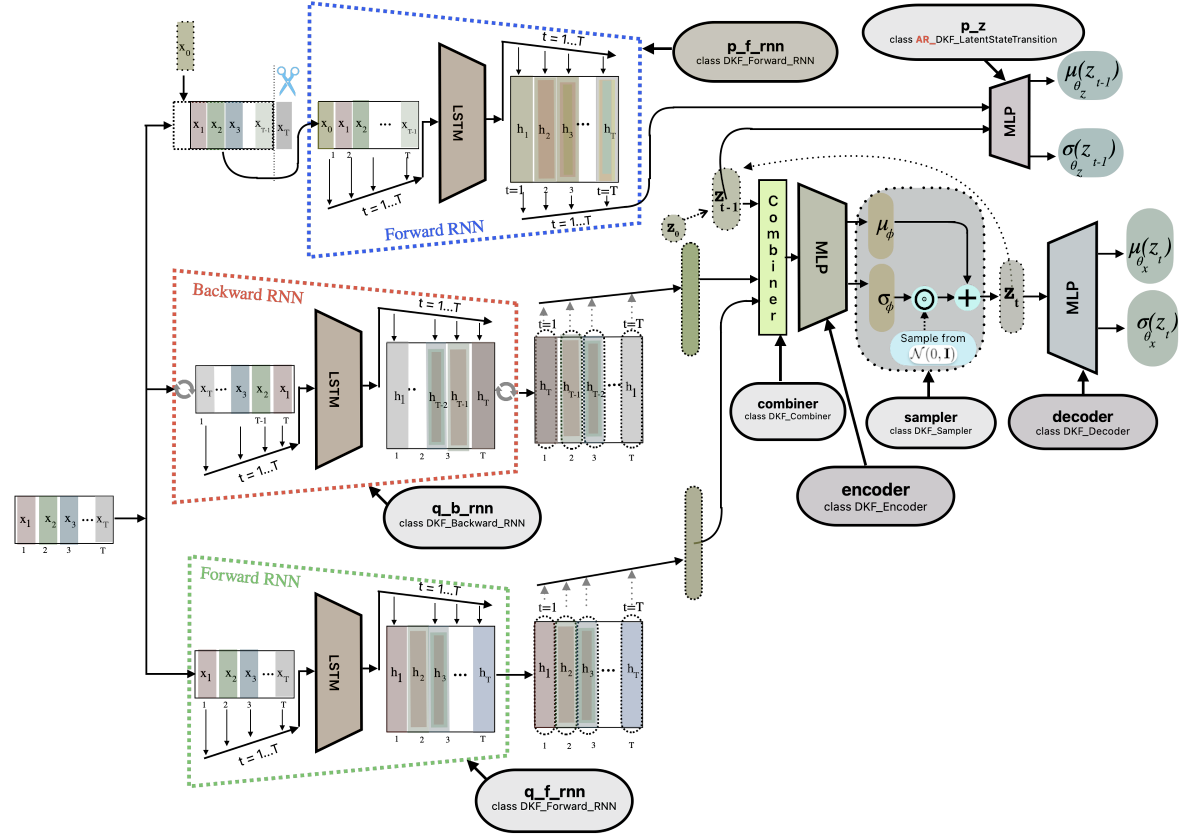
\includegraphics[width=480px]{./Images/far_dkf_implementation_objects.png}
    \caption{FAR DKF: the forward RNN \code{q\_f\_rnn} feeds the
    combiner of the inference network.}
    \label{fig:far_dkf_implementation_objects}
\end{figure}

\subsection{Bidirectional Autoregressive DKF (BAR DKF)}

The BAR DKF replaces the backward RNN of the inference network by a
single bidirectional RNN, whose output at time $t$ combines a summary of
$\mathbf{x}_{1:t}$ and a summary of $\mathbf{x}_{t:T}$. Its inference
model therefore also has the form $q_\phi(\mathbf{z}_t \mid
\mathbf{z}_{t-1}, \mathbf{x}_{1:T})$, with fewer parameters than the FAR
DKF because the two directions are merged before the combiner.

\subsection{Summary}

All three autoregressive variants share the generative model
\eqref{eq:ar_generative}. They differ in their inference networks:
\begin{center}
\begin{tabular}{|l|l|l|}
\hline
\textbf{Model} & \textbf{Inference network} & \textbf{Matches the
posterior structure?} \\ \hline
AR DKF & $q_\phi(\mathbf{z}_t \mid \mathbf{z}_{t-1}, \mathbf{x}_{t:T})$
& No: ignores $\mathbf{x}_{1:t-1}$ \\ \hline
FAR DKF & $q_\phi(\mathbf{z}_t \mid \mathbf{z}_{t-1}, \mathbf{x}_{1:T})$,
two RNNs & Yes \\ \hline
BAR DKF & $q_\phi(\mathbf{z}_t \mid \mathbf{z}_{t-1}, \mathbf{x}_{1:T})$,
one bidirectional RNN & Yes \\ \hline
\end{tabular}
\end{center}
On the Lorenz data, over four training runs per experiment, the three
variants reconstruct the observations equally well, and none of them
forecasts consistently better than the others. Their ELBOs on test data
vary more between runs of the same model than between models, and the
estimated ELBO gaps are the same for the three variants
(Appendix~\ref{sec:results}). The advantage that
Proposition~\ref{prop:ar_posterior} suggests for the FAR DKF and the BAR
DKF is therefore not visible in these experiments.

\chapter{Conclusion}

The Deep Kalman Filter keeps the probabilistic structure of the Kalman
filter, a Markov chain of latent states with one emission per time step,
and makes the transition and emission non-linear with neural networks.
Exact inference is then impossible, and the model is trained like a VAE,
by maximising a lower bound on the log-likelihood.\\

Three points that the original paper leaves implicit are central to
understanding the method:
\begin{itemize}
    \item \textbf{The structure of the inference network follows from
    d-separation.} Given $\mathbf{z}_{t-1}$, the true posterior of
    $\mathbf{z}_t$ depends only on the future observations
    $\mathbf{x}_{t:T}$, which is why the inference network combines
    $\mathbf{z}_{t-1}$ with a backward RNN.
    \item \textbf{The ELBO splits into one KL per time step}, by the
    chain rule of the KL divergence. Each of these is between two
    Gaussians given $\mathbf{z}_{t-1}$ and has a closed form.
    \item \textbf{One sampled trajectory gives an unbiased estimate of
    the ELBO.} The ELBO is linear in its expectations under the
    intractable marginals of the inference network, and ancestral
    sampling provides exact samples of all of these marginals at once.
\end{itemize}

The autoregressive variants I designed add edges from past observations
to the latent state, which gives the transition model direct access to
the history and greatly improves forecasting on the sine-wave data.
Redoing the d-separation argument on the new graph shows that these
edges also change the posterior: it now depends on the past observations
as well as the future ones. The FAR DKF, whose inference network sees
both, is therefore the principled inference model for the AR DKF
generative model. On the Lorenz data, however, the three autoregressive
variants perform comparably: over four training runs per experiment,
neither the forecasting errors nor the ELBOs on test data rank them
consistently, and the variability between runs is larger than the
differences between models.\\

Several directions remain open. The variability between training runs
should be reduced, or at least controlled with fixed random seeds and
more repetitions, before the variants can be compared. Tighter estimates
of the log-likelihood, with many more importance samples, would be
needed to measure the differences between their ELBO gaps.
Forecasts should be evaluated with the predictive mean, or with a
probabilistic score, rather than with a single sampled path. The
reconstruction error currently matches the noise level, which suggests
that the inference network reproduces the observations, noise included,
rather than denoising them: monitoring the two terms of the ELBO
separately would show how much of the ELBO each part of the model
accounts for. Finally, control inputs, for example from an inertial
measurement unit, could be added to the transition model as in the
original formulation.


\begin{appendices}
\renewcommand{\thesection}{\Alph{section}}
\section{Understanding the Backward LSTM}\label{sec:backward_lstm}

The inference network needs, at each time step $t$, a summary of the
future observations $\mathbf{x}_{t:T}$. A backward RNN provides all of
them in a single pass.

\subsection*{Definition}

A backward LSTM is an ordinary LSTM run from $t = T$ down to $t = 1$. Its
state at time $t$ is computed from the observation $\mathbf{x}_t$ and the
state at time $t+1$:
\begin{align*}
    \mathbf{f}_t &= \sigma(\mathbf{W}_f [\mathbf{b}_{t+1}, \mathbf{x}_t]
    + \mathbf{c}_f) & &\text{(forget gate)}\\
    \mathbf{i}_t &= \sigma(\mathbf{W}_i [\mathbf{b}_{t+1}, \mathbf{x}_t]
    + \mathbf{c}_i) & &\text{(input gate)}\\
    \tilde{\mathbf{m}}_t &= \tanh(\mathbf{W}_m [\mathbf{b}_{t+1},
    \mathbf{x}_t] + \mathbf{c}_m) & &\text{(candidate memory)}\\
    \mathbf{m}_t &= \mathbf{f}_t \odot \mathbf{m}_{t+1} + \mathbf{i}_t
    \odot \tilde{\mathbf{m}}_t & &\text{(memory cell)}\\
    \mathbf{o}_t &= \sigma(\mathbf{W}_o [\mathbf{b}_{t+1}, \mathbf{x}_t]
    + \mathbf{c}_o) & &\text{(output gate)}\\
    \mathbf{b}_t &= \mathbf{o}_t \odot \tanh(\mathbf{m}_t) & &
    \text{(output)}
\end{align*}
with initial values $\mathbf{b}_{T+1} = \mathbf{0}$ and
$\mathbf{m}_{T+1} = \mathbf{0}$. Here $\sigma$ is the logistic sigmoid,
$[\cdot, \cdot]$ denotes concatenation, and the $\mathbf{W}$'s and
$\mathbf{c}$'s are learned weights and biases.

\begin{inwords}
Unrolling the recursion, $\mathbf{b}_t$ is a function of
$\mathbf{x}_t, \mathbf{x}_{t+1}, \dots, \mathbf{x}_T$ only. So
$\mathbf{b}_t$ summarises exactly the suffix $\mathbf{x}_{t:T}$ that the
posterior factor $q_\phi(\mathbf{z}_t \mid \mathbf{z}_{t-1},
\mathbf{x}_{t:T})$ needs. At $t = T$ it has seen only $\mathbf{x}_T$, and
at $t = 1$ it has seen the whole sequence.
\end{inwords}

\subsection*{Implementation by flipping}

Deep-learning libraries implement LSTMs that run forwards in time. The
backward LSTM is obtained by flipping the sequence, running a forward
LSTM, and flipping the outputs back:
\begin{enumerate}
    \item flip: $(\mathbf{x}_T, \mathbf{x}_{T-1}, \dots, \mathbf{x}_1)$;
    \item run the LSTM: its $k$-th output, $k = 1, \dots, T$, has seen
    $\mathbf{x}_T, \dots, \mathbf{x}_{T-k+1}$;
    \item flip the outputs back: the output now stored at position
    $t = T - k + 1$ has seen $\mathbf{x}_{t:T}$, i.e.\ it is
    $\mathbf{b}_t$.
\end{enumerate}
This is what \code{DKF\_Backward\_RNN} does, with
\code{torch.flip} along the time dimension (dimension 0, since tensors
have shape \code{(seq\_len, batch\_size, dim)}).

\begin{figure}[ht!]
    \centering
    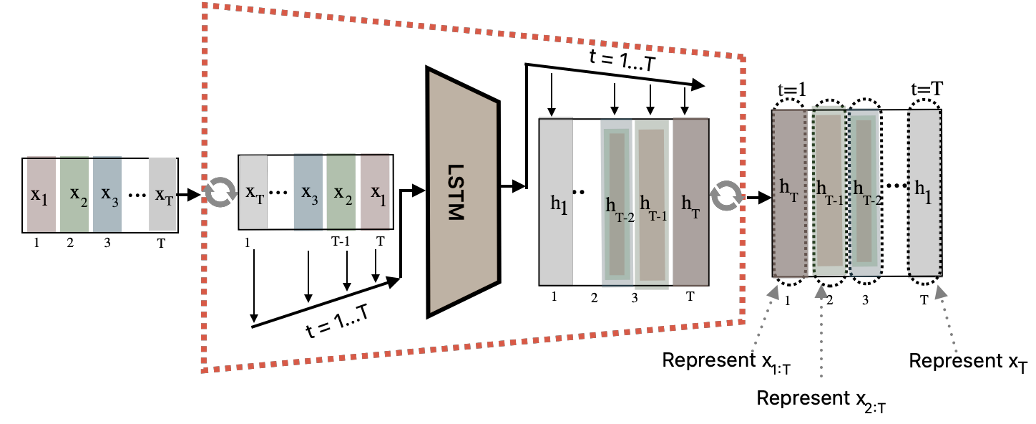
\includegraphics[width=400px]{./Images/backward_lstm.png}
    \caption{Backward LSTM. In this figure the hidden states are indexed
    by their position in the \emph{flipped} sequence: $h_k$ is
    $\mathbf{b}_{T-k+1}$ in the notation of this appendix.}
    \label{fig:backward_lstm}
\end{figure}


\pagebreak
\section{Detailed Derivation of the ELBO}\label{sec:elbo_derivation}

\begin{story}[Notation]
As in the main text, $p_{\theta}(\mathbf{z}_{1} \mid \mathbf{z}_{0},
\star)$ is the prior on $\mathbf{z}_1$, and $q_{\phi}(\mathbf{z}_{1}
\mid \mathbf{z}_{0}, \star)$ is the first factor of the inference
network, with $\mathbf{z}_0$ fixed or learned. To lighten the formulas,
$q$ stands for $q_\phi(\cdot \mid \mathbf{x}_{1:T}, \mathbf{u}_{1:T})$
and its factors, and $p$ for $p_\theta$.
\end{story}

\subsection*{Step 1: the bound}

As for the VAE (Chapter~\ref{chap:vae}), Jensen's inequality gives
\begin{equation*}
    \log p(\mathbf{x}_{1:T} \mid \mathbf{u}_{1:T}) \;\geq\;
    \mathcal{L} := \E_{q(\mathbf{z}_{1:T})}\left[\log
    \frac{p(\mathbf{x}_{1:T}, \mathbf{z}_{1:T} \mid \mathbf{u}_{1:T})}
    {q(\mathbf{z}_{1:T})}\right],
\end{equation*}
with a gap equal to $\KL\big(q(\mathbf{z}_{1:T}) \,\|\,
p(\mathbf{z}_{1:T} \mid \mathbf{x}_{1:T}, \mathbf{u}_{1:T})\big)$.

\subsection*{Step 2: substitute the factorisations}

With the generative model \eqref{eq:generative_model} and the inference
model \eqref{q_phi},
\begin{equation*}
    \log \frac{p(\mathbf{x}_{1:T}, \mathbf{z}_{1:T} \mid \mathbf{u}_{1:T})}
    {q(\mathbf{z}_{1:T})} =
    \sum_{t=1}^T \log p(\mathbf{x}_t \mid \mathbf{z}_t)
    \;-\; \sum_{t=1}^T \underbrace{\log \frac{q(\mathbf{z}_t \mid
    \mathbf{z}_{t-1}, \mathbf{x}_{t:T}, \mathbf{u}_{t:T})}
    {p(\mathbf{z}_t \mid \mathbf{z}_{t-1}, \mathbf{u}_t)}}_{=:\ r_t(
    \mathbf{z}_{t-1}, \mathbf{z}_t)}.
\end{equation*}
By linearity of expectation,
\begin{equation}
    \mathcal{L} = \sum_{t=1}^T \E_{q(\mathbf{z}_{1:T})}\big[\log
    p(\mathbf{x}_t \mid \mathbf{z}_t)\big] - \sum_{t=1}^T
    \E_{q(\mathbf{z}_{1:T})}\big[r_t(\mathbf{z}_{t-1}, \mathbf{z}_t)\big].
    \label{eq:elbo_step2}
\end{equation}
Each term depends on one or two consecutive latent states only. The next
step shows how to integrate out all the others.

\subsection*{Step 3: integrating out the latent states a term does not
depend on}

\begin{proposition}\label{prop:marginalise}
For any functions $f$ and $g$,
\begin{align*}
    \E_{q(\mathbf{z}_{1:T})}\big[f(\mathbf{z}_t)\big] &=
    \E_{q(\mathbf{z}_t)}\big[f(\mathbf{z}_t)\big], \\
    \E_{q(\mathbf{z}_{1:T})}\big[g(\mathbf{z}_{t-1}, \mathbf{z}_t)\big] &=
    \E_{q(\mathbf{z}_{t-1})}\Big[\E_{q(\mathbf{z}_t \mid
    \mathbf{z}_{t-1}, \mathbf{x}_{t:T}, \mathbf{u}_{t:T})}\big[
    g(\mathbf{z}_{t-1}, \mathbf{z}_t)\big]\Big],
\end{align*}
where $q(\mathbf{z}_t)$ and $q(\mathbf{z}_{t-1})$ denote the marginals of
the inference model.
\end{proposition}

\begin{proof}
Write the expectation as an integral against
$q(\mathbf{z}_{1:T}) = \prod_{s=1}^T q(\mathbf{z}_s \mid
\mathbf{z}_{s-1}, \mathbf{x}_{s:T}, \mathbf{u}_{s:T})$.

\emph{Future states.} The integrand does not depend on $\mathbf{z}_T$
(when $t < T$), and $\mathbf{z}_T$ appears only in the last factor, which
is a probability density in $\mathbf{z}_T$. Hence
\[
    \int q(\mathbf{z}_T \mid \mathbf{z}_{T-1}, \mathbf{x}_{T},
    \mathbf{u}_{T})\,d\mathbf{z}_T = 1,
\]
and $\mathbf{z}_T$ disappears. Repeating the argument for
$\mathbf{z}_{T-1}, \dots, \mathbf{z}_{t+1}$ removes all future states.
What remains is the integral against
$q(\mathbf{z}_{1:t}) = \prod_{s=1}^{t} q(\mathbf{z}_s \mid
\mathbf{z}_{s-1}, \cdot)$, the marginal of the first $t$ states.

\emph{Past states.} Split $q(\mathbf{z}_{1:t}) =
q(\mathbf{z}_{1:t-1})\, q(\mathbf{z}_t \mid \mathbf{z}_{t-1},
\mathbf{x}_{t:T}, \mathbf{u}_{t:T})$. The inner integral over
$\mathbf{z}_t$ is the inner expectation in the statement. The resulting
function of $\mathbf{z}_{t-1}$ is then integrated against
$q(\mathbf{z}_{1:t-1})$. Integrating out $\mathbf{z}_{1:t-2}$, on which
it does not depend, gives the marginal $q(\mathbf{z}_{t-1})$ by
definition of a marginal. For $f(\mathbf{z}_t)$, integrating out
$\mathbf{z}_{1:t-1}$ in the same way gives $q(\mathbf{z}_t)$.
\end{proof}

\begin{story}[About the factor $q(\mathbf{z}_t \mid \mathbf{z}_{1:t-1},
\cdot)$]
The proof uses $q(\mathbf{z}_t \mid \mathbf{z}_{1:t-1}, \mathbf{x}_{1:T},
\mathbf{u}_{1:T}) = q(\mathbf{z}_t \mid \mathbf{z}_{t-1},
\mathbf{x}_{t:T}, \mathbf{u}_{t:T})$. This holds \emph{by construction}
of the inference model \eqref{q_phi}: the inference network is built to
receive only these inputs. D-separation is what justified that design,
because the true posterior has the same property; but in the derivation
itself, the equality is a property of $q$, not a d-separation statement.
\end{story}

\subsection*{Step 4: the result}

Apply Proposition~\ref{prop:marginalise} to \eqref{eq:elbo_step2}, with
$f = \log p(\mathbf{x}_t \mid \cdot)$ and $g = r_t$. For the second
term, the inner expectation is a KL divergence:
\begin{equation*}
    \E_{q(\mathbf{z}_t \mid \mathbf{z}_{t-1}, \mathbf{x}_{t:T},
    \mathbf{u}_{t:T})}\big[r_t(\mathbf{z}_{t-1}, \mathbf{z}_t)\big] =
    \KL\big(q(\mathbf{z}_t \mid \mathbf{z}_{t-1}, \mathbf{x}_{t:T},
    \mathbf{u}_{t:T}) \,\big\|\, p(\mathbf{z}_t \mid \mathbf{z}_{t-1},
    \mathbf{u}_{t})\big).
\end{equation*}
Therefore
\begin{equation*}
\boxed{
\begin{aligned}
    \mathcal{L} =\ & \sum_{t=1}^T \E_{q_\phi(\mathbf{z}_{t} \mid
    \mathbf{x}_{1:T}, \mathbf{u}_{1:T})} \big[\log p_\theta(\mathbf{x}_t
    \mid \mathbf{z}_{t})\big] \\
    & - \sum_{t=1}^T \E_{q_\phi(\mathbf{z}_{t-1} \mid \mathbf{x}_{1:T},
    \mathbf{u}_{1:T})} \Big[ \KL\big(q_\phi(\mathbf{z}_t \mid
    \mathbf{z}_{t-1}, \mathbf{x}_{t:T}, \mathbf{u}_{t:T}) \,\big\|\,
    p_\theta(\mathbf{z}_t \mid \mathbf{z}_{t-1}, \mathbf{u}_{t})\big)
    \Big],
\end{aligned}
}
\end{equation*}
which is \eqref{eq:dkf_elbo}. The second sum is the \emph{chain rule}
of the KL divergence: for two Markov chains,
\begin{equation*}
    \KL\big(q(\mathbf{z}_{1:T}) \,\|\, p(\mathbf{z}_{1:T})\big) =
    \sum_{t=1}^T \E_{q(\mathbf{z}_{t-1})}\Big[\KL\big(q(\mathbf{z}_t
    \mid \mathbf{z}_{t-1}) \,\|\, p(\mathbf{z}_t \mid \mathbf{z}_{t-1})
    \big)\Big].
\end{equation*}

\subsection*{Remark: iterated expectations}

Applying the proof of Proposition~\ref{prop:marginalise} to all time
steps writes the expectation under $q(\mathbf{z}_{1:T})$ as
\emph{iterated} conditional expectations,
\begin{equation*}
    \E_{q(\mathbf{z}_{1:T})}[h] =
    \E_{q(\mathbf{z}_1 \mid \mathbf{z}_0, \cdot)}\Big[
    \E_{q(\mathbf{z}_2 \mid \mathbf{z}_1, \cdot)}\big[ \cdots
    \E_{q(\mathbf{z}_T \mid \mathbf{z}_{T-1}, \cdot)}[h] \cdots \big]
    \Big].
\end{equation*}
Each inner expectation is passed to the next level as it is, with no
non-linear function applied to it, so the iterated expectations collapse
into a single expectation over the joint distribution (the tower
property). That is why ancestral sampling, one sample per level, gives
an unbiased estimate (Proposition~\ref{prop:unbiased}).


\pagebreak
\section{Detailed Mathematical Development of the Reconstruction Term}
\label{sec:elbo_recon}
%
\subsection*{Problem Setup}

Given the probability distribution:
\begin{equation*}
    p_{\theta_{\bm{x}}}(\bm{x}_t | \bm{z}_{t}) = 
    \mathcal{N}(\bm{x}_t; \mu_{\theta_{\bm{x}}}(\bm{z}_{t}), 
    \Sigma^2_{\theta_{\bm{x}}}(\bm{z}_{t}))
\end{equation*}

where $\Sigma^2_{\theta_{\bm{x}}}(\bm{z}_{t}) = 
diag(\sigma^2_{\theta_{\bm{x}}}(\bm{z}_{t}))$,
we aim to develop the expression:

\begin{equation*}
    \sum_{t=1}^T \Big[ \log p_\theta(x_t | z_{t}) \Big]
\end{equation*}

\subsection*{Logarithm of the Probability Distribution}
The probability density function (PDF) of a multivariate normal 
distribution $\mathcal{N}(\bm{x}_t; \mu_{\theta_{\bm{x}}}(\bm{z}_{t}), 
\Sigma^2_{\theta_{\bm{x}}}(\bm{z}_{t}))$ is given by:
%
\begin{equation*}
    p_{\theta_{\bm{x}}}(\bm{x}_t | \bm{z}_{t}) = 
    \frac{1}{(2\pi)^{d/2} 
    \big|\Sigma^2_{\theta_{\bm{x}}}(\bm{z}_{t}) \big|^{1/2}} 
    \exp\left(-\frac{1}{2} \big(\bm{x}_t - 
    \mu_{\theta_{\bm{x}}}(\bm{z}_{t})\big)^\top 
    \big(\Sigma^2_{\theta_{\bm{x}}}(\bm{z}_{t})\big)^{-1} \big(\bm{x}_t - 
    \mu_{\theta_{\bm{x}}}(\bm{z}_{t})\big)\right)    
\end{equation*}
%
\newline
In this context, \(d\) represents the dimensionality of the random variable 
\(\bm{x}_t\). Specifically, \(\bm{x}_t\) is a \(d\)-dimensional vector, 
and \(\mu_{\theta_{\bm{x}}}(\bm{z}_{t})\) is also a \(d\)-dimensional vector. 
The covariance matrix \(\Sigma^2_{\theta_{\bm{x}}}(\bm{z}_{t})\) is a 
\(d \times d\) diagonal matrix, where 
each diagonal element corresponds to the variance of one dimension of \(\bm{x}_t\).\\
%
\newline
%
Taking the logarithm, we get:
\begin{equation*}
    \log p_{\theta_{\bm{x}}}(\bm{x}_t | \bm{z}_{t}) = 
    -\frac{d}{2} \log(2\pi) - \frac{1}{2} \log 
    \big|\Sigma^2_{\theta_{\bm{x}}}(\bm{z}_{t})\big| - 
    \frac{1}{2} \big(\bm{x}_t - \mu_{\theta_{\bm{x}}}(\bm{z}_{t})\big)^\top 
    \big(\Sigma^2_{\theta_{\bm{x}}}(\bm{z}_{t})\big)^{-1} 
    \big(\bm{x}_t - \mu_{\theta_{\bm{x}}}(\bm{z}_{t})\big)
\end{equation*}


\subsection*{Simplify the Logarithm Expression}
Given that 
\(\Sigma^2_{\theta_{\bm{x}}}(\bm{z}_{t}) = 
diag(\sigma^2_{\theta_{\bm{x}}}(\bm{z}_{t}))\), we have:
\begin{equation*}
    \log |\Sigma^2_{\theta_{\bm{x}}}(\bm{z}_{t})| = 
    \log \prod_{i=1}^d \sigma^2_{\theta_{\bm{x}}, i}(\bm{z}_{t}) = 
    \sum_{i=1}^d \log \sigma^2_{\theta_{\bm{x}}, i}(\bm{z}_{t})
\end{equation*}

and
\begin{equation*}
    (\Sigma^2_{\theta_{\bm{x}}}(\bm{z}_{t}))^{-1} = 
    \begin{pmatrix}
    \frac{1}{\sigma^2_{\theta_{\bm{x}}, 1}(\bm{z}_{t})} & 0 & \cdots & 0 \\
    0 & \frac{1}{\sigma^2_{\theta_{\bm{x}}, 2}(\bm{z}_{t})} & \cdots & 0 \\
    \vdots & \vdots & \ddots & \vdots \\
    0 & 0 & \cdots & \frac{1}{\sigma^2_{\theta_{\bm{x}}, d}(\bm{z}_{t})}
    \end{pmatrix}
\end{equation*}

Thus,
\begin{equation*}
    \big(\bm{x}_t - \mu_{\theta_{\bm{x}}}(\bm{z}_{t})\big)^\top 
    \big(\Sigma^2_{\theta_{\bm{x}}}(\bm{z}_{t})\big)^{-1} 
    \big(\bm{x}_t - \mu_{\theta_{\bm{x}}}(\bm{z}_{t})\big) = 
    \sum_{i=1}^d \frac{\big(x_{t,i} - \mu_{\theta_{\bm{x}}, i}(\bm{z}_{t})\big)^2}
    {\sigma^2_{\theta_{\bm{x}}, i}(\bm{z}_{t})}
\end{equation*}

and
\begin{equation}
    \log p_{\theta_{\bm{x}}}(\bm{x}_t | \bm{z}_{t}) = 
    -\frac{d}{2} \log(2\pi) - 
    \frac{1}{2} \sum_{i=1}^d \log \sigma^2_{\theta_{\bm{x}}, i}(\bm{z}_{t}) - 
    \frac{1}{2} \sum_{i=1}^d \frac{\big(x_{t,i} - \mu_{\theta_{\bm{x}}, i}(\bm{z}_{t})\big)^2}
    {\sigma^2_{\theta_{\bm{x}}, i}(\bm{z}_{t})}\label{eq:log_p_theta_x_given_z}
\end{equation}

\subsection*{Summing Over Time Steps}
Now, we sum over all time steps \(t\) from 1 to \(T\):
\begin{equation*}
    \sum_{t=1}^T \log p_{\theta_{\bm{x}}}(\bm{x}_t | \bm{z}_{t}) = 
    \sum_{t=1}^T \left[ -\frac{d}{2} \log(2\pi) - 
    \frac{1}{2} \sum_{i=1}^d \log \sigma^2_{\theta_{\bm{x}}, i}(\bm{z}_{t}) - 
    \frac{1}{2} \sum_{i=1}^d \frac{\big(x_{t,i} - \mu_{\theta_{\bm{x}}, i}(\bm{z}_{t})\big)^2}
    {\sigma^2_{\theta_{\bm{x}}, i}(\bm{z}_{t})} \right]
\end{equation*}

\subsection*{Final Expression}
\begin{equation}
    \sum_{t=1}^T \log p_{\theta_{\bm{x}}}(\bm{x}_t | \bm{z}_{t}) = 
    - \frac{Td}{2} \log(2\pi) - \frac{1}{2} \sum_{t=1}^T 
    \sum_{i=1}^d \left[ \log \sigma^2_{\theta_{\bm{x}}, i}(\bm{z}_{t}) +
    \frac{\big(x_{t,i} - \mu_{\theta_{\bm{x}}, i}(\bm{z}_{t})\big)^2}
    {\sigma^2_{\theta_{\bm{x}}, i}(\bm{z}_{t})} \right]
    \label{eq:sum_log_p_theta_x_given_z}
\end{equation}
\noindent In the estimator \eqref{eq:elbo_estimator}, this expression is
evaluated at the sampled latent states $\dot{\bm{z}}_{1:T}$. The first
term, $-\frac{Td}{2}\log(2\pi)$, does not depend on the parameters and is
dropped from the loss (Section~\ref{sec:loss}).

\pagebreak
\section{Detailed Mathematical Development of the Regularization Term}
\label{sec:elbo_regularization}
(Computation is done here without the control input term $\bm{u}$.)
%
\subsection*{Problem Setup}

Given the following distributions:

\begin{equation*}
    p_{\theta_{\bm{z}}}(\bm{z}_t | \bm{z}_{t-1}) 
    = 
    \mathcal{N}(\bm{z}_t; 
    \mu_{\theta_{\bm{z}}}(\bm{z}_{t-1}), 
    \Sigma^2_{\theta_{\bm{z}}}(\bm{z}_{t-1}))
    =
    \mathcal{N}(\bm{z}_t; 
    \mu_{\theta_{\bm{z}}}(\bm{z}_{t-1}), 
    \text{diag}(\sigma^2_{\theta_{\bm{z}}}(\bm{z}_{t-1})))
\end{equation*}

and
\begin{equation*}
    q_{\phi}(\bm{z}_t | \bm{z}_{t-1}, \bm{x}_{t:T}) 
    = 
    \mathcal{N}(\bm{z}_t; \mu_{\phi}(\bm{z}_{t-1}, \bm{x}_{t:T}), 
    \Sigma^2_{\phi}(\bm{z}_{t-1}, \bm{x}_{t:T}))
    =
    \mathcal{N}(\bm{z}_t; \mu_{\phi}(\bm{z}_{t-1}, \bm{x}_{t:T}), 
    \text{diag}(\sigma^2_{\phi}(\bm{z}_{t-1}, \bm{x}_{t:T})))
\end{equation*}

We aim to compute:
%
\begin{equation*}
    \sum_{t=1}^T 
    \KL
    \big(
    q_\phi(z_t | z_{t-1}, x_{t:T})
    \parallel
    p_\theta(z_t | z_{t-1})
    \big)
\end{equation*}

\subsection*{KL Divergence Between Two Gaussian Distributions}

The KL divergence between two multivariate Gaussian distributions
$ \mathcal{N}(\bm{z}; \bm{\mu}_1, \Sigma_1) $ and 
$ \mathcal{N}(\bm{z}; \bm{\mu}_2, \Sigma_2) $ is given by:

\begin{equation*}
\KL \big( \mathcal{N}(\bm{z}; \bm{\mu}_1, \Sigma_1) 
\parallel \mathcal{N}(\bm{z}; \bm{\mu}_2, \Sigma_2) \big) = 
\frac{1}{2} \left( \text{tr}(\Sigma_2^{-1} \Sigma_1) + 
(\bm{\mu}_2 - \bm{\mu}_1)^T \Sigma_2^{-1} (\bm{\mu}_2 - \bm{\mu}_1) 
- k + \log \frac{|\Sigma_2|}{|\Sigma_1|} \right)
\end{equation*}

where $k$ is the dimensionality of the Gaussian distributions.

\subsection*{Simplification for Diagonal Covariance Matrices}

Since both $q_\phi$ and $p_\theta$ are diagonal Gaussian distributions,
their covariance matrices are diagonal. Let's denote:

\begin{equation*}
\Sigma_{\phi} = \text{diag}\big(\sigma^2_{\phi}(\bm{z}_{t-1}, 
\bm{x}_{t:T})\big)
\end{equation*}
\begin{equation*}
\Sigma_{\theta} = \text{diag}\big(\sigma^2_{\theta_{\bm{z}}}
(\bm{z}_{t-1})\big)
\end{equation*}

For diagonal matrices, the trace and determinant operations simplify:

\begin{equation*}
\text{tr}(\Sigma_{\theta}^{-1} \Sigma_{\phi}) = \sum_{i} 
\frac{\sigma^2_{\phi, i}(\bm{z}_{t-1}, \bm{x}_{t:T})}
{\sigma^2_{\theta_{\bm{z}}, i}(\bm{z}_{t-1})}
\end{equation*}
\begin{equation*}
\log \frac{|\Sigma_{\theta}|}{|\Sigma_{\phi}|} = 
\sum_{i} \log \frac{\sigma^2_{\theta_{\bm{z}}, i}(\bm{z}_{t-1})}
{\sigma^2_{\phi, i}(\bm{z}_{t-1}, \bm{x}_{t:T})}
\end{equation*}

\subsection*{Final Computation}

The KL divergence for each time step $t$ is:

\begin{align*}
\KL\big( q_\phi(\bm{z}_t | \bm{z}_{t-1}, \bm{x}_{t:T}) 
\parallel p_\theta(\bm{z}_t | \bm{z}_{t-1}) \big) = 
\frac{1}{2} \Bigg(& 
    \sum_{i} \frac{\sigma^2_{\phi, i}(\bm{z}_{t-1}, \bm{x}_{t:T})}
    {\sigma^2_{\theta_{\bm{z}}, i}(\bm{z}_{t-1})} \quad + \\
    & \sum_{i} \left( \mu_{\theta_{\bm{z}}, i}(\bm{z}_{t-1}) - 
    \mu_{\phi, i}(\bm{z}_{t-1}, \bm{x}_{t:T}) \right)^2 \frac{1}
    {\sigma^2_{\theta_{\bm{z}}, i}(\bm{z}_{t-1})} - k \quad + \\
    & \sum_{i} \log \frac{\sigma^2_{\theta_{\bm{z}}, i}(\bm{z}_{t-1})}
    {\sigma^2_{\phi, i}(\bm{z}_{t-1}, \bm{x}_{t:T})} \Bigg)
\end{align*}

Summing over all time steps $t = 1, \dots, T$:

\begin{equation*}
\sum_{t=1}^T \KL\big( q_\phi(\bm{z}_t | \bm{z}_{t-1}, 
\bm{x}_{t:T})
\parallel p_\theta(\bm{z}_t | \bm{z}_{t-1}) \big) = 
\end{equation*}
\begin{equation}
    \frac{1}{2} \sum_{t=1}^T \left( 
        \sum_{i} \left( 
            \frac{\sigma^2_{\phi, i}(\bm{z}_{t-1}, \bm{x}_{t:T})}{\sigma^2_{\theta_{\bm{z}}, i}(\bm{z}_{t-1})} 
            + \frac{(\mu_{\theta_{\bm{z}}, i}(\bm{z}_{t-1}) - \mu_{\phi, i}(\bm{z}_{t-1}, \bm{x}_{t:T}))^2}{\sigma^2_{\theta_{\bm{z}}, i}(\bm{z}_{t-1})} 
            - 1 
            + \log \frac{\sigma^2_{\theta_{\bm{z}}, i}(\bm{z}_{t-1})}{\sigma^2_{\phi, i}(\bm{z}_{t-1}, \bm{x}_{t:T})} 
        \right)
    \right)\label{eq:regularization_term}
\end{equation}
\noindent In the estimator \eqref{eq:elbo_estimator}, each term of this sum
is evaluated at the sampled previous state $\dot{\bm{z}}_{t-1}$, both in
the parameters of $q_\phi$ and in those of $p_{\theta_{\bm{z}}}$. The
term $-1$ inside the sum contributes the constant $-\frac{T d_z}{2}$,
where $d_z$ is the dimension of $\bm{z}_t$. It does not depend on the
parameters, which is why it can be dropped from the loss
(Section~\ref{sec:loss}).

\pagebreak
\section{Combiner in the Deep Kalman Filter (DKF)}\label{combiner_info}
    
The \textbf{Combiner} is a key component in the DKF model, responsible 
for integrating information from different sources to produce a unified 
representation. Specifically, it combines the previous latent state 
($\bm{z}_{t-1}$) with the hidden states of one or more Recurrent Neural 
Networks (RNNs) to create an output that is fed into the encoder. 
This output is then used to compute the parameters of the latent 
distribution ($\bm{z}_t$).

\subsection*{Purpose of the Combiner}

The Combiner's primary role is to:
\begin{enumerate}
    \item \textbf{Integrate Information}: Combine the previous latent 
    state ($\bm{z}_{t-1}$) with the hidden states of RNNs (e.g., backward RNN, 
    forward RNN) to create a richer representation.
    \item \textbf{Produce a Unified Output}: Generate a single tensor that 
    can be fed into the encoder to compute the mean and log variance of the 
    latent state ($\bm{z}_t$).
    \item \textbf{Flexibility}: Allow for different ways of combining 
    information, such as linear combination or using a Multi-Layer 
    Perceptron (MLP).
\end{enumerate}

\subsection*{Key Concepts}

\begin{itemize}
    \item \textbf{Latent State ($\bm{z}_{t-1}$)}:
        \begin{itemize}
            \item The latent state from the previous time step, which 
            represents the hidden variables of the model.\\
            At $t=1$, $\bm{z}_0$ is either a fix tensor of zeros or a learnable
            parameter initialiazed with zeros.
        \end{itemize}
    \item \textbf{RNN Hidden States ($\bm{h}_{t}^{i}$)}:
        \begin{itemize}
            \item The output of one or more RNNs (e.g., backward RNN, 
            forward RNN) that process the input sequence. These hidden 
            states capture temporal dependencies in the data.
        \end{itemize}
    \item \textbf{Combination Strategy}:
        \begin{itemize}
            \item The method used to combine $\bm{z}_{t-1}$ with the RNN 
            hidden states. This can be a simple linear combination or 
            a more complex MLP-based combination.
        \end{itemize}
\end{itemize}

\subsection*{Combiner Types}

The Combiner is implemented in two main ways:
\begin{enumerate}
    \item \textbf{Linear Combiner}: Combines $\bm{z}_{t-1}$ and RNN hidden 
    states using a weighted sum (linear combination).
    \item \textbf{MLP Combiner}: Combines $\bm{z}_{t-1}$ and RNN hidden 
    states using a Multi-Layer Perceptron (MLP).
\end{enumerate}

\subsection{Linear Combiner}

The \textbf{Linear Combiner} performs a weighted sum of the previous 
latent state ($\bm{z}_{t-1}$) and the RNN hidden states. 
The weights are controlled by a parameter $\alpha_i$, which determines 
the contribution of each input.

\subsubsection*{Key Parameters}
\begin{itemize}
    \item \code{$z\_dim$}: Dimension of the latent state ($\bm{z}_{t-1}$).
    \item \code{$rnn\_dims$}: Dimensions of the RNN hidden states. 
    This can be a single dimension or a list of dimensions if multiple 
    RNNs are used.
    \item \code{$output\_dim$}: Dimension of the output tensor.
    \item \code{$\alpha^i$}: Weight for the $i$-th RNN hidden state. 
    This determines how much influence the mapped $\bm{z}_{t-1}$ has on 
    the combination.
\end{itemize}

\subsubsection*{Formula}

\begin{equation*}
    \bm{combined}^{i}_{t} = \alpha^{i} \cdot \text{mapped}(\bm{z}_{t-1}) + 
    (1 - \alpha^{i}) \cdot \bm{h}_{t}^{i}
\end{equation*}

Where:

\begin{itemize}
    \item $\text{mapped}(\bm{z}_{t-1}) = \tanh(\mathbf{W}^i \bm{z}_{t-1}
    + \mathbf{c}^i)$: the previous latent state mapped to the dimension of
    the $i$-th RNN hidden state by a linear layer followed by the
    activation function ($\tanh$ in all experiments).
    \item $\bm{h}_{t}^{i}$: The hidden state output of the $i$-th RNN
    at time $t$.
\end{itemize}

With a single RNN and $\alpha = 0.5$, this is the combiner of Krishnan
et al.'s follow-up work \cite{krishnan2017structured},
$\frac{1}{2}\big(\tanh(\mathbf{W}\bm{z}_{t-1} + \mathbf{c}) +
\bm{h}_t\big)$, followed by a linear layer.

Two sets of weights are kept: \code{alpha\_init}, meant for the first
time step, where $\bm{z}_{0}$ is a fixed or learned constant that carries
no information about the sequence, and \code{alpha}, used for the
following steps.

\subsubsection*{How It Works}
\begin{enumerate}
    \item \textbf{Mapping $\bm{z}_{t-1}$}:
        \begin{itemize}
            \item The previous latent state ($\bm{z}_{t-1}$) is mapped to
            the dimension of each RNN hidden state by separate linear
            layers, each followed by the activation function.
        \end{itemize}
    \item \textbf{Weighted Sum}:
        \begin{itemize}
            \item The mapped $\bm{z}_{t-1}$ and the RNN hidden state are 
            combined using a weighted sum. The weight $\alpha^i$ 
            controls the contribution of the mapped $\bm{z}_{t-1}$, while 
            $(1 - \alpha^i)$ controls the contribution of the RNN hidden 
            state.
        \end{itemize}
    \item \textbf{Concatenation}:
        \begin{itemize}
            \item The combined tensors for all RNN hidden states are 
            concatenated along the feature dimension.
        \end{itemize}
    \item \textbf{Final Linear Layer}:
        \begin{itemize}
            \item The concatenated tensor is passed through a final linear
            layer to produce the output tensor of dimension \code{output\_dim}.
        \end{itemize}
\end{enumerate}

\subsubsection*{Example}
Suppose:

\begin{itemize}
    \item $\alpha^i = 0.3$
    \item $\text{mapped}(\bm{z}_{t-1}) = \bm{mz}$
    \item $\bm{h}_{t}^{i} = \bm{rnn\_h}$
\end{itemize}

The formula becomes:

\begin{align*}
    \bm{combined}^i &= 0.3 \cdot \bm{mz} + 
    (1 - 0.3) \cdot \bm{rnn\_h} \\
    &= 0.3 \cdot \bm{mz} + 0.7 \cdot \bm{rnn\_h}
\end{align*}

This means:
\begin{itemize}
    \item 30\% of the contribution comes from the mapped latent state 
    $\text{mapped}$.
    \item 70\% of the contribution comes from the RNN hidden state 
    \code{rnn\_h}.
\end{itemize}

\subsection{MLP Combiner}

The \textbf{MLP Combiner} uses a Multi-Layer Perceptron (MLP) to combine
the previous latent state ($\bm{z}_{t-1}$) and the RNN hidden states.
This allows for more complex interactions between the inputs.

\subsubsection*{Key Parameters}
\begin{itemize}
    \item \code{z\_dim}: Dimension of the latent state ($\bm{z}_{t-1}$).
    \item \code{rnn\_dims}: Dimensions of the RNN hidden states.
    \item \code{output\_dim}: Dimension of the output tensor.
    \item \code{layers\_dim}: List of dimensions for the hidden
    layers in the MLP.
    \item \code{activation}: Activation function 
    (e.g., $\tanh$ or $\text{ReLU}$).
\end{itemize}

\subsubsection*{How It Works}
\begin{enumerate}
    \item \textbf{Concatenation}:
        \begin{itemize}
            \item The previous latent state ($\bm{z}_{t-1}$) and all RNN hidden
            states are concatenated along the feature dimension.
        \end{itemize}
    \item \textbf{MLP Layers}:
        \begin{itemize}
            \item The concatenated tensor is passed through a series of
            linear layers with activation functions in between.
            \item The first layer maps the concatenated input to the first
            hidden layer dimension.
            \item Intermediate layers map the output of one hidden layer to
            the next.
            \item The final layer maps the last hidden layer to the output
            dimension (\code{output\_dim}).
        \end{itemize}
    \item \textbf{Output}:
        \begin{itemize}
            \item The output of the MLP is the combined tensor, which is
            then fed into the encoder.
        \end{itemize}
\end{enumerate}

\subsubsection{Example}
Suppose:
\begin{itemize}
    \item $\bm{z}_{t-1}$ has a dimension of 16.
    \item Two RNN hidden states: $h^1_t$ (dimension 32) and $h^2_t$ (dimension 64).
\end{itemize}
%
The concatenated input will have a dimension of \(16 + 32 + 64 = 112\).
This concatenated tensor is passed through an MLP.

\subsection{Combiner Factory}

The \textbf{Combiner Factory} is a utility class that creates the
appropriate Combiner based on the specified type ($\text{linear}$ or
$\text{mlp}$). This allows for flexibility in choosing the combination
strategy.

\subsubsection*{Key Parameters}

\begin{itemize}
    \item \code{combiner\_type}: Type of Combiner to use 
    (\text{linear} or \text{mlp}).
    \item \textbf{Other Parameters}: Depend on the type of Combiner 
    (e.g., \code{$\alpha^i$}, \code{layers\_dim}).
\end{itemize}

\subsubsection*{How It Works}

\begin{itemize}
    \item If \code{combiner\_type} = \code{linear}, the factory 
    initializes a \code{DKF\_CombinerLinear} with the specified parameters.
    \item If \code{combiner\_type} = \code{mlp}, the factory initializes 
    a \code{DKF\_CombinerMLP} with the specified parameters.
\end{itemize}
\subsection{Summary of the Combiner's Role in the DKF}

The Combiner is responsible for integrating the previous latent state
($\bm{z}_{t-1}$) with the hidden states of RNNs to produce a unified
representation. This representation is then used by the encoder to
compute the parameters of the latent distribution ($\bm{z}_{t}$).
The Combiner can be either a simple linear combination or a more complex
MLP-based combination, depending on the model's requirements.
\\
By using the Combiner, the DKF model can effectively leverage both the
temporal dependencies captured by RNNs and the latent state dynamics to
model complex time series data.

\pagebreak
\section{Results of Deep Kalman Filter Models}\label{sec:results}

This appendix presents the results of the vanilla DKF and of the AR DKF,
FAR DKF and BAR DKF on two kinds of data: simple sine waves, and windows
of a trajectory of the Lorenz attractor. Gaussian noise is added to the
observed part of each sequence. The model reconstructs that part and then
forecasts the following steps.

\subsection*{How to read these results}

\begin{itemize}
    \item \textbf{Errors are measured against the clean signal.} The
    reconstruction and prediction MSEs compare the model's output with
    the ground truth \emph{before} noise was added. The \enquote{MSE of
    the noise} is the error one would make by simply returning the noisy
    input.
    \item \textbf{Reconstruction at the noise level means no
    denoising.} For all the models, the reconstruction MSE is close to
    the MSE of the noise. In the figures, the
    reconstruction follows the noisy input point by point rather than the
    clean curve. The inference network passes each observation, noise
    included, through the latent state, and the decoder reproduces it.
    A good reconstruction MSE is therefore \emph{not} evidence that the
    model has learned the dynamics; the forecasting error is the
    informative quantity.
    \item \textbf{Forecasts are single sampled paths.} \code{predict}
    samples one latent trajectory and one path of the dynamics. Its error
    includes sampling noise and would be lower for the mean of the
    predictive distribution.
    \item \textbf{Repeated runs.} Each Lorenz experiment was trained
    four times. The figures of each dataset show the first run; the
    summary at the end of this appendix gives the mean and the spread
    over the four runs. The sine-wave experiments were trained once.
\end{itemize}

\subsection*{DKF with Simple Sine Waves}

The vanilla DKF was tested on two sine-wave datasets with different
frequencies. It follows the observed part of the sequences closely, but
its forecasts lose track of the signal. With $f=1$ they flatten out and
lose the amplitude; with $f=2$ they keep oscillating at roughly the right
frequency but drift out of phase within one or two periods. The
transition model alone has not learned the periodic dynamics.

\begin{figure}[ht!]
    \centering
    \begin{subfigure}[b]{0.49\textwidth}
        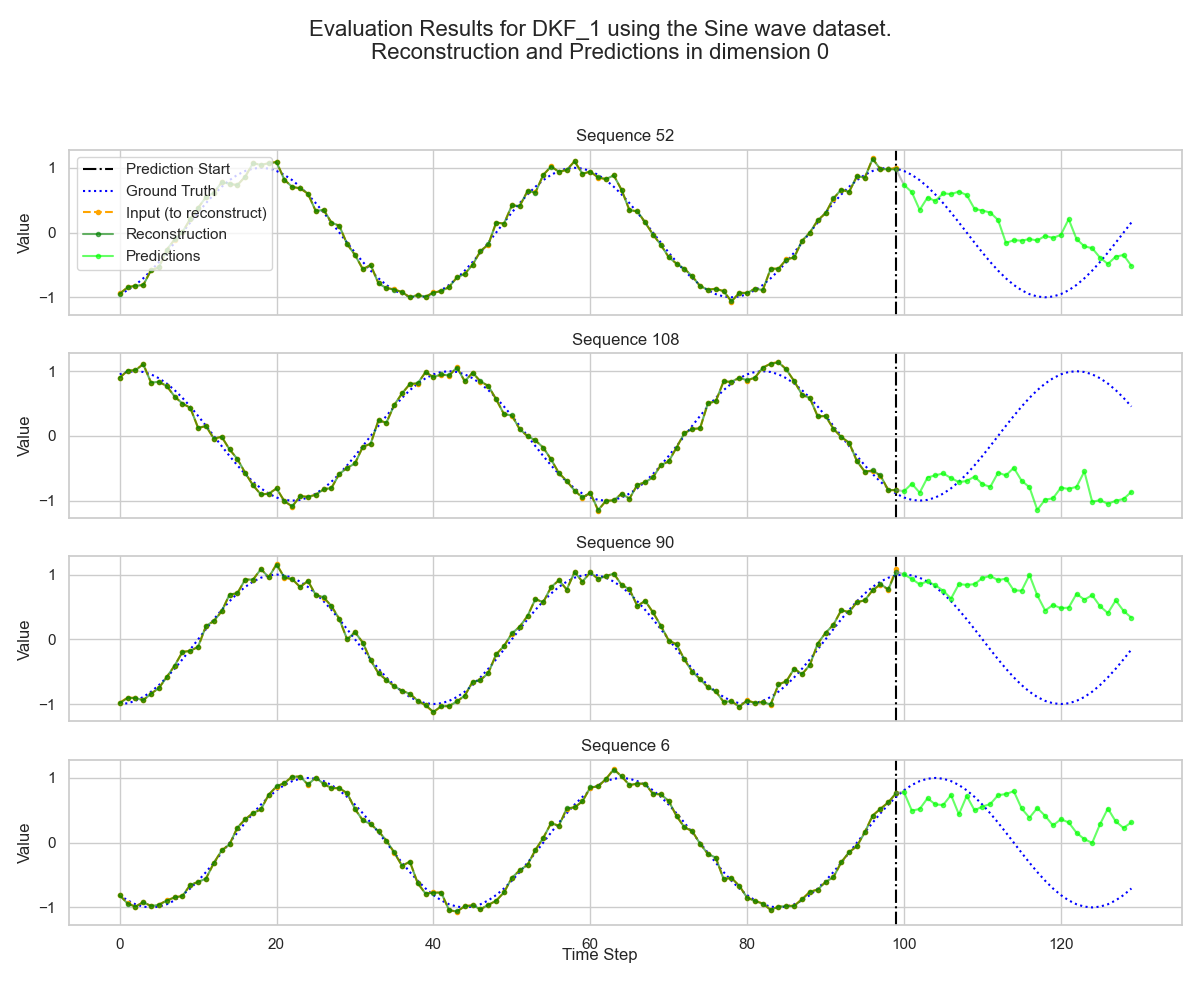
\includegraphics[width=\textwidth]{./Images/DKF_sine_wave_1.png}
        \caption{DKF on sine wave with $f=1$.}
        \label{fig:dkf_sine_wave_1}
    \end{subfigure}
    \hfill
    \begin{subfigure}[b]{0.49\textwidth}
        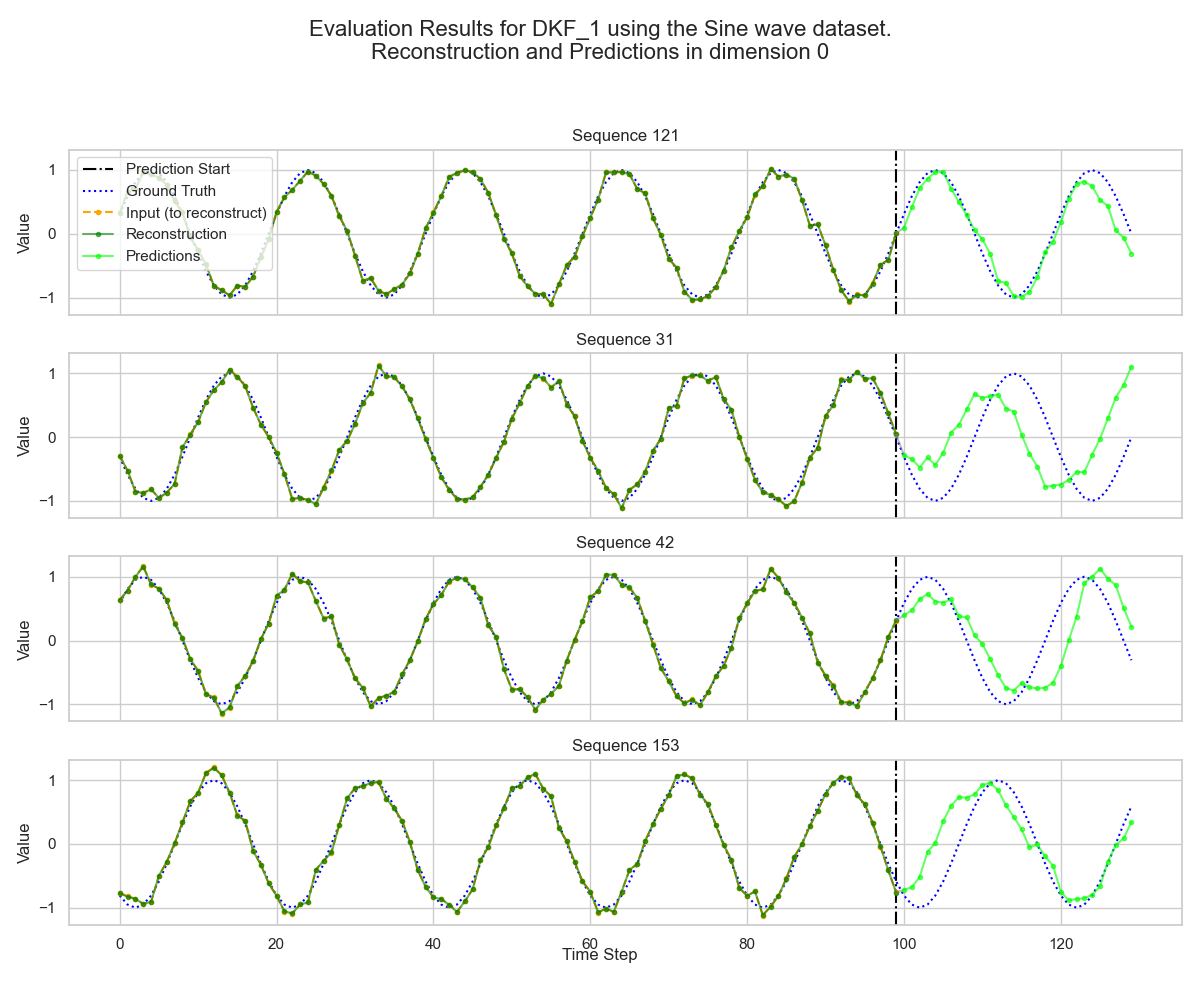
\includegraphics[width=\textwidth]{./Images/DKF_sine_wave_2.png}
        \caption{DKF on sine wave with $f=2$.}
        \label{fig:dkf_sine_wave_2}
    \end{subfigure}
    \caption{DKF reconstruction and prediction on two sine-wave
    datasets.}
    \label{fig:dkf_sine_wave_results}
\end{figure}

\subsection*{AR DKF with Simple Sine Waves}
    
    The AR DKF was tested on the same sine wave datasets as
    for the DKF.
    The AR DKF forecasts both sine waves far better than the vanilla DKF:
    the forecasts keep the phase, the frequency and the amplitude of the
    signal over the whole prediction window. The prediction MSE is
    $0.876$ for the DKF and $0.0052$ for the AR DKF with $f=1$, and
    $0.571$ and $0.0094$ with $f=2$ (Figure~\ref{fig:sine_mse_comparison}).
    For a sine wave of amplitude 1, always predicting $0$ would give an MSE
    of $0.5$: on both datasets the DKF forecasts are worse than this
    trivial predictor, while the AR DKF forecasts have an error of the
    same order as the noise of the observations.
    The difference is large enough to be conclusive even with a single
    run. It supports the idea behind the AR DKF: giving the transition
    model direct access to the history lets it carry the information
    needed for forecasting.
    
    \begin{figure}[ht!]
        \centering
        \begin{subfigure}[b]{0.49\textwidth}
            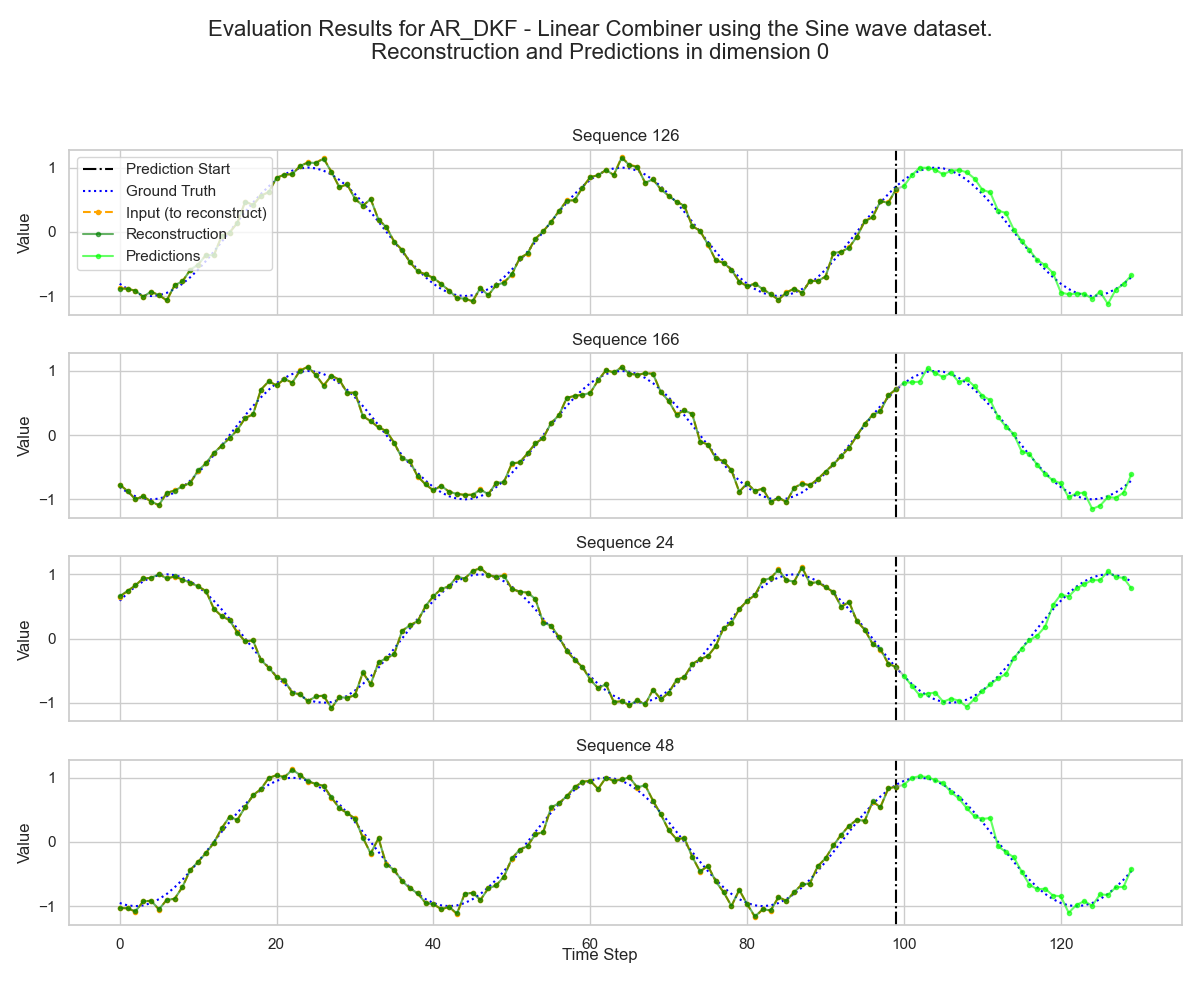
\includegraphics[width=\textwidth]{./Images/AR_DKF_sine_wave_1.png}
            \caption{AR DKF on sine wave with $f=1$.}
            \label{fig:ar_dkf_sine_wave_1}
        \end{subfigure}
        \hfill
        \begin{subfigure}[b]{0.49\textwidth}
            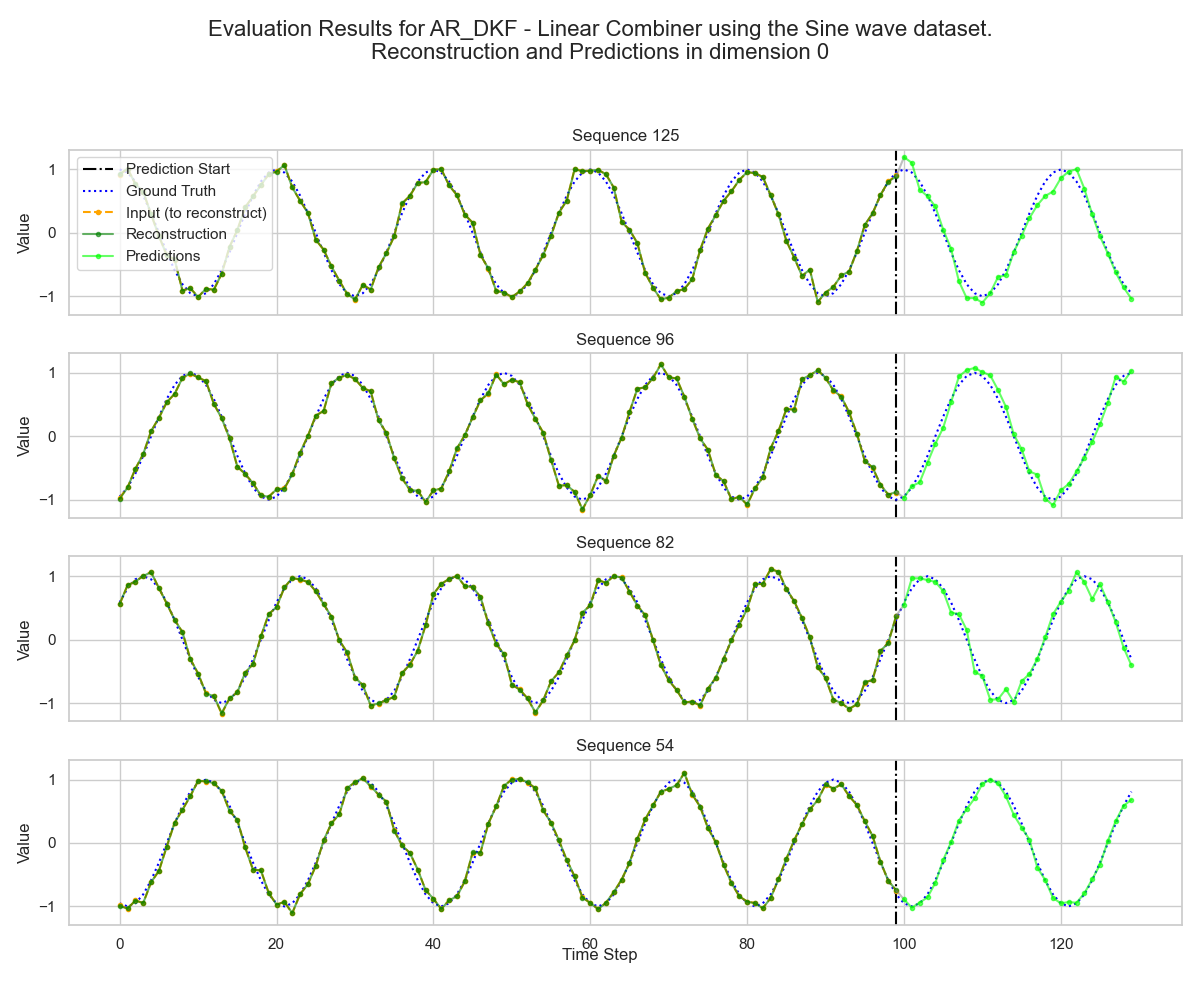
\includegraphics[width=\textwidth]{./Images/AR_DKF_sine_wave_2.png}
            \caption{AR DKF on sine wave with $f=2$.}
            \label{fig:ar_dkf_sine_wave_2}
        \end{subfigure}
        \caption{Examples of AR DKF Reconstruction and Prediction
        on two simple sine wave datasets.}
        \label{fig:ar_dkf_sine_wave_results}
    \end{figure}

    \begin{figure}[ht!]
        \centering
        \begin{subfigure}[b]{0.49\textwidth}
            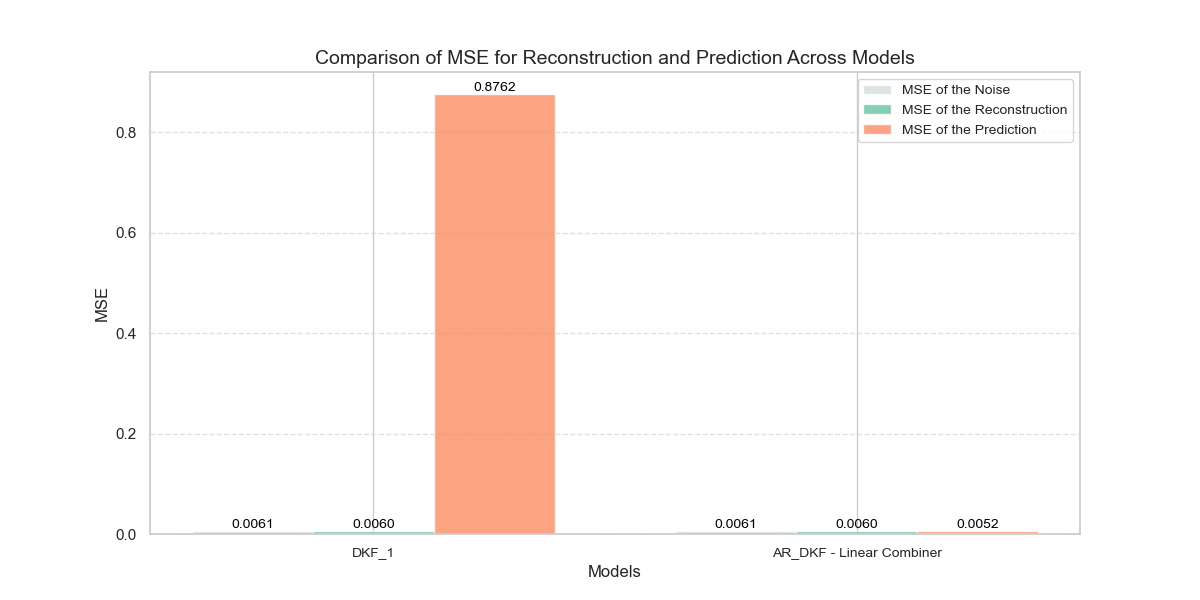
\includegraphics[width=\textwidth]{./Images/sine_mse_comparison_1.png}
            \caption{Sine wave with $f=1$.}
        \end{subfigure}
        \hfill
        \begin{subfigure}[b]{0.49\textwidth}
            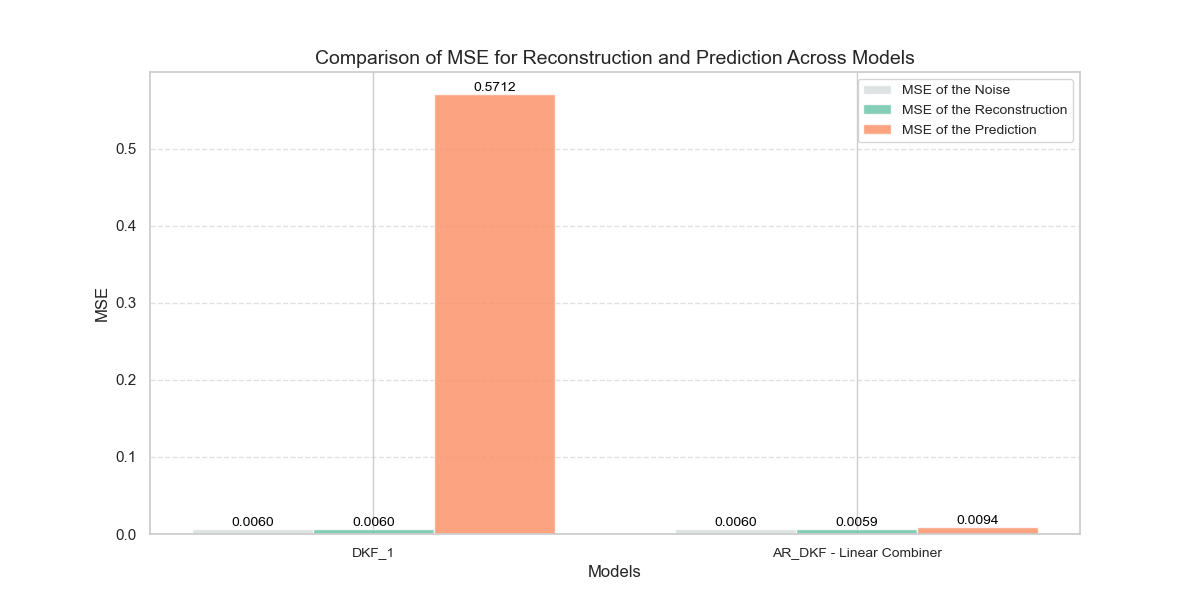
\includegraphics[width=\textwidth]{./Images/sine_mse_comparison_2.png}
            \caption{Sine wave with $f=2$.}
        \end{subfigure}
        \caption{Reconstruction and prediction MSE of the DKF and the
        AR DKF on the two sine-wave datasets.}
        \label{fig:sine_mse_comparison}
    \end{figure}
    
    \subsection*{Comparison of AR DKF, FAR DKF, and
    BAR DKF on Lorenz Attractor}
    
    The AR DKF, FAR DKF, and BAR DKF
    were compared using three sets of data from the Lorenz attractor.
    The datasets were designed to test the models' ability to
    generalize under varying degrees of dissimilarity between training
    and testing data. Each experiment was repeated four times with the
    same settings; the figures below show the first run.
    
    \subsubsection*{Configurations}
    All the subsequent results are obtained with configurations
    given in the tables below.\\
    
    %- - - - - - - - - - - - - - - - - - - - - - - - - - - - 
    \begin{minipage}{0.48\textwidth}
        \centering
        \small
        \label{tab:args_config}
        \captionof{table}{Args Configuration}
        \begin{tabular}{|l|l|}
        \hline
        \textbf{Parameter} & \textbf{Value} \\ \hline
        dataset & lorenz \\ \hline
        lorenz\_initial\_point & 2, 1, 1 \\ \hline
        lorenz\_points & 20000 \\ \hline
        lorenz\_range & Dataset 1: [4500, 6500] \\
        & Dataset 2: [8600, 10500]\\
        & Dataset 3: [11000, 13000]\\ \hline
        loss\_function & weighted\_mse \\ \hline
        noise\_var & 0.006 \\ \hline
        normalization\_type & standardize \\ \hline
        train\_seq\_len & 100 \\ \hline
        test\_seq\_len (prediction) & 100 \\ \hline
        \end{tabular}
     %\end{table}
    \end{minipage}
    \hfill
    \begin{minipage}{0.45\textwidth}
        \centering
            \label{tab:training_config_config}
            \captionof{table}{Training Configuration}
            \begin{tabular}{|l|l|}
            \hline
            \textbf{Parameter} & \textbf{Value} \\ \hline
            learning\_rate & 0.001 \\ \hline
            num\_epochs & 120 \\ \hline
            pred\_batch\_size & 32 \\ \hline
            train\_batch\_size & 32 \\ \hline
            val\_batch\_size & 16 \\ \hline
            \end{tabular}
        %\end{table} 
    \end{minipage}
    
    \begin{table}[h!]
    \centering
    \caption{Models Configuration}
    \label{tab:models_config_config}
    \begin{tabular}{|l|l|l|l|}
    \hline
    \diagbox[width=\dimexpr \textwidth/4 + 4\tabcolsep\relax,height=0.7cm]
    {\textbf{Parameter}}{\textbf{Model}}
    & \textbf{AR DKF} & \textbf{FAR DKF} & 
    \textbf{BAR DKF} \\ \hline
    activation & tanh & tanh & tanh \\ \hline
    combiner\_alpha & 0.5 & 0.5, 0.5 & 0.5 \\ \hline
    combiner\_alpha\_init & 0.1 & 0.1, 0.1 & 0.1 \\ \hline
    combiner\_layers\_dim & 64 & 64 & 64 \\ \hline
    combiner\_learnable\_alpha & Yes & Yes, Yes & Yes \\ \hline
    combiner\_output\_dim & 64 & 64 & 64 \\ \hline
    combiner\_type & linear & linear & linear \\ \hline
    decoder\_layers\_dim & 64, 32 & 64, 32 & 64, 32 \\ \hline
    device & cpu & cpu & cpu \\ \hline
    dropout\_p & 0.0 & 0.0 & 0.0 \\ \hline
    encoder\_layers\_dim & 64 & 64 & 64 \\ \hline
    latent\_transition\_layers\_dim & 64 & 64 & 64 \\ \hline
    learnable\_init\_x & No & No & No \\ \hline
    learnable\_init\_z & Yes & Yes & Yes \\ \hline
    pz\_f\_rnn\_hidden\_size & 64 & 64 & 64 \\ \hline
    pz\_f\_rnn\_num\_layers & 1 & 1 & 1 \\ \hline
    q\_b\_rnn\_hidden\_size & 64 & 64 & 64 \\ \hline
    q\_b\_rnn\_num\_layers & 1 & 1 & 1 \\ \hline
    x\_dim & 3 & 3 & 3 \\ \hline
    z\_dim & 16 & 16 & 16 \\ \hline
    q\_f\_rnn\_hidden\_size &  & 64 &  \\ \hline
    q\_f\_rnn\_num\_layers &  & 1 &  \\ \hline
    
    \end{tabular}
    \end{table}
    
    %- - - - - - - - - - - - - - - - - - - - - - - - - - - - 
    
    \subsubsection*{Dataset 1}
    
    The dataset (\textit{before the addition of Gaussian noise}) is shown
    in the figure \ref{fig:dataset_1_partial_data} below.\\
    
    \begin{figure}[ht!]
        \centering
        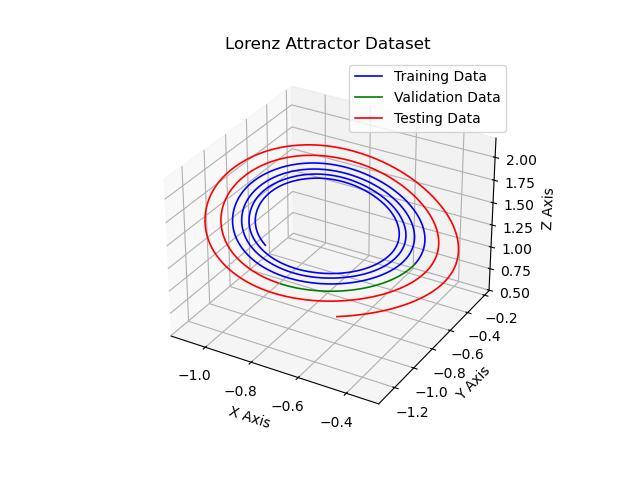
\includegraphics[width=0.75\textwidth]
        {./Images/Dataset_1/partial_data.png}
        \caption{Lorenz attractor - Range [4500, 6500] }
        \label{fig:dataset_1_partial_data}
    \end{figure}
    %
    \FloatBarrier
    
    Figure \ref{fig:dataset_1_AR_DKF_1_all_dims} below shows the results
    of the AR DKF model for four sequences from the dataset in
    each dimension.
    
    \begin{figure}[ht!]
        \centering
        \begin{minipage}{0.31\textwidth}
            \centering
            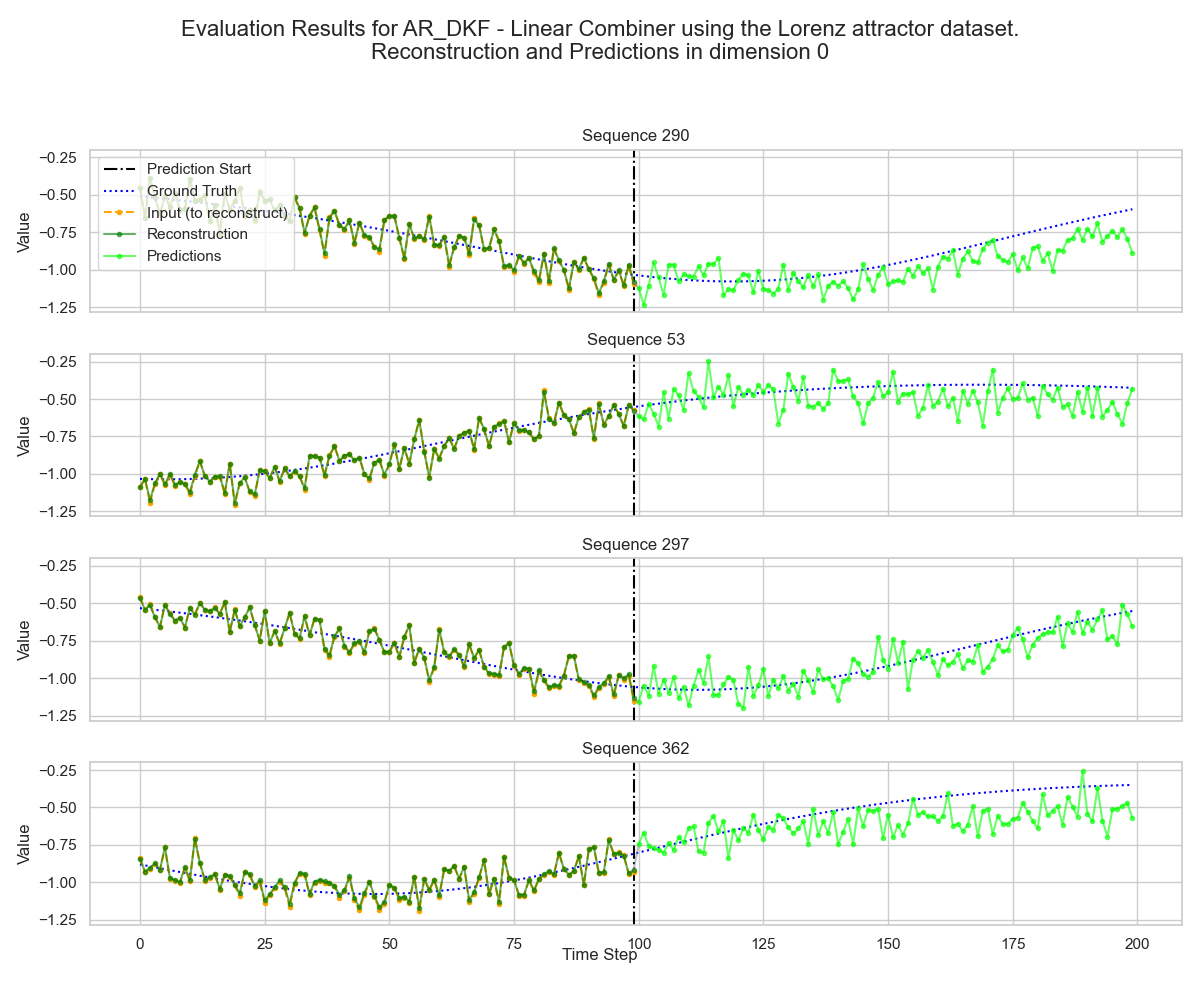
\includegraphics[width=1\textwidth]{./Images/Dataset_1/AR_DKF_1_dim_0.png}
            \subcaption{Reconstruction and Prediction in the 1st dimension.}
            \label{fig:dataset_1_AR_DKF_1_dim_0}
        \end{minipage}
        \hfill
        \begin{minipage}{0.31\textwidth}
            \centering
            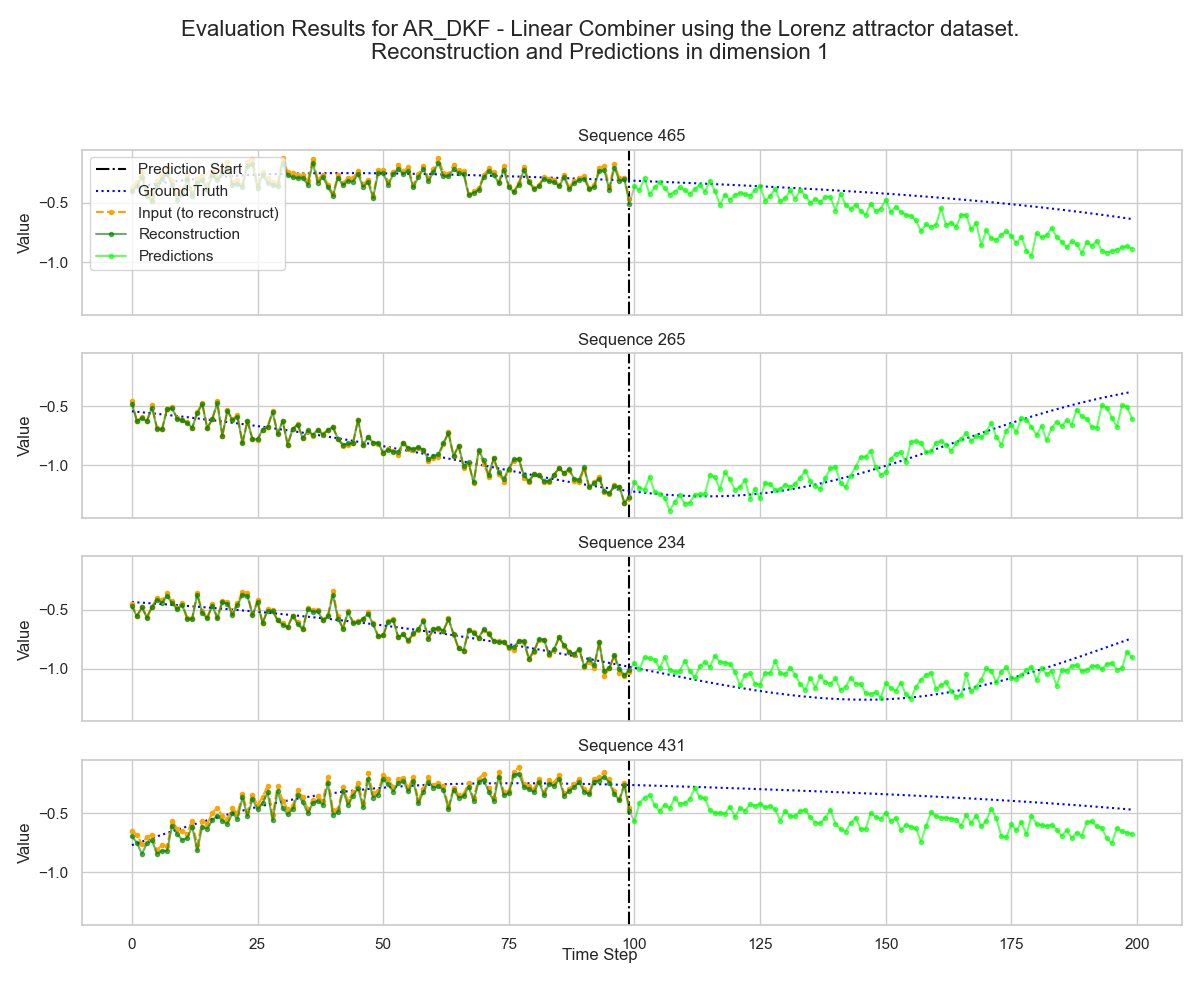
\includegraphics[width=1\textwidth]{./Images/Dataset_1/AR_DKF_1_dim_1.png}
            \subcaption{Reconstruction and Prediction in the 2nd dimension.}
            \label{fig:dataset_1_AR_DKF_1_dim_1}
        \end{minipage}
        \hfill
        \begin{minipage}{0.31\textwidth}
            \centering
            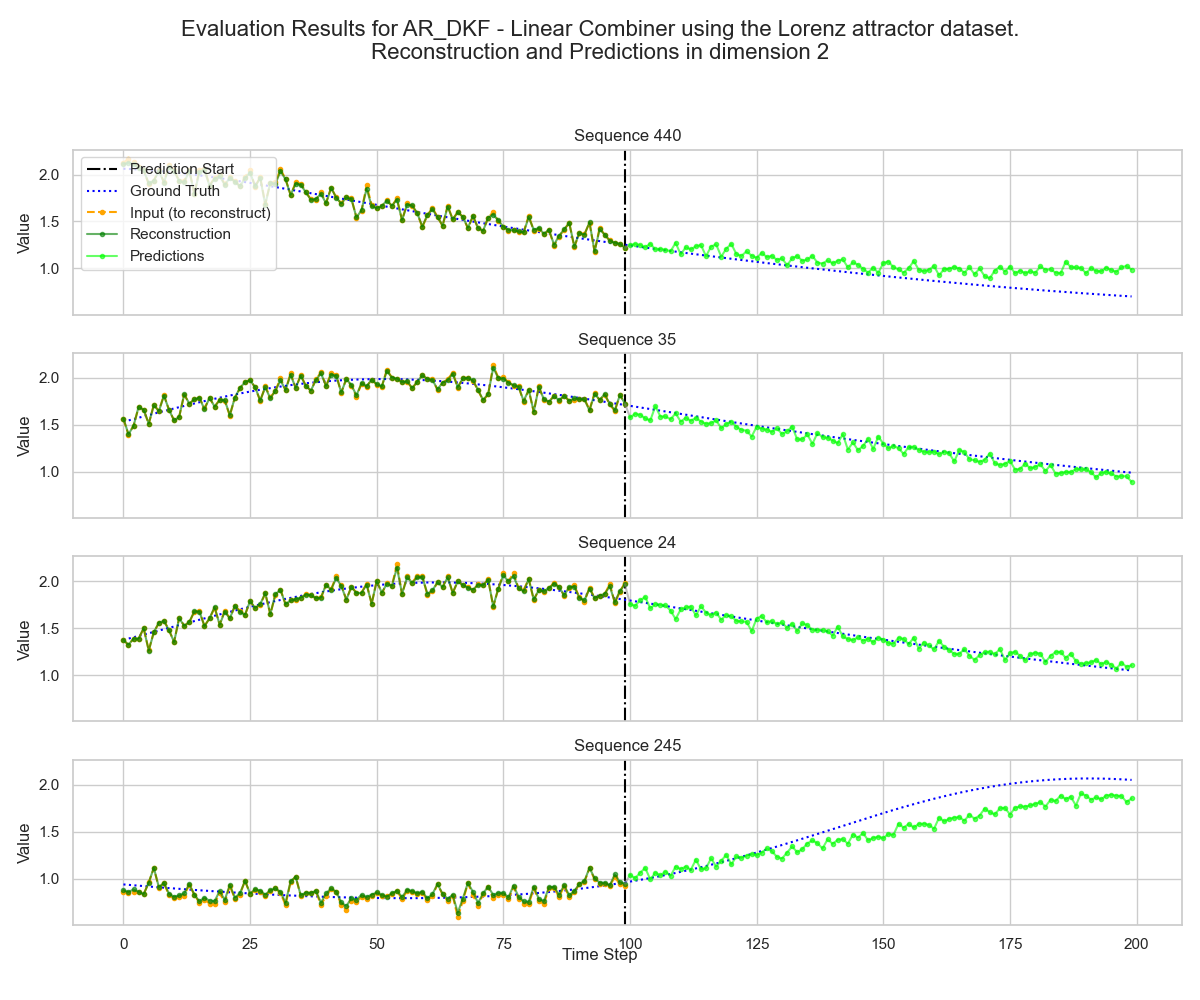
\includegraphics[width=1\textwidth]{./Images/Dataset_1/AR_DKF_1_dim_2.png}
            \subcaption{Reconstruction and Prediction in the 3rd dimension.}
            \label{fig:dataset_1_AR_DKF_1_dim_2}
        \end{minipage}
        \caption{Examples of Reconstruction and Prediction for the
        AR DKF model.}
        \label{fig:dataset_1_AR_DKF_1_all_dims}
    \end{figure}
    
    Figure \ref{fig:dataset_1_FAR_DKF_1_all_dims} below shows the results
    of the FAR DKF model on the same sequences.
    
    \begin{figure}[ht!]
        \centering
        \begin{minipage}{0.31\textwidth}
            \centering
            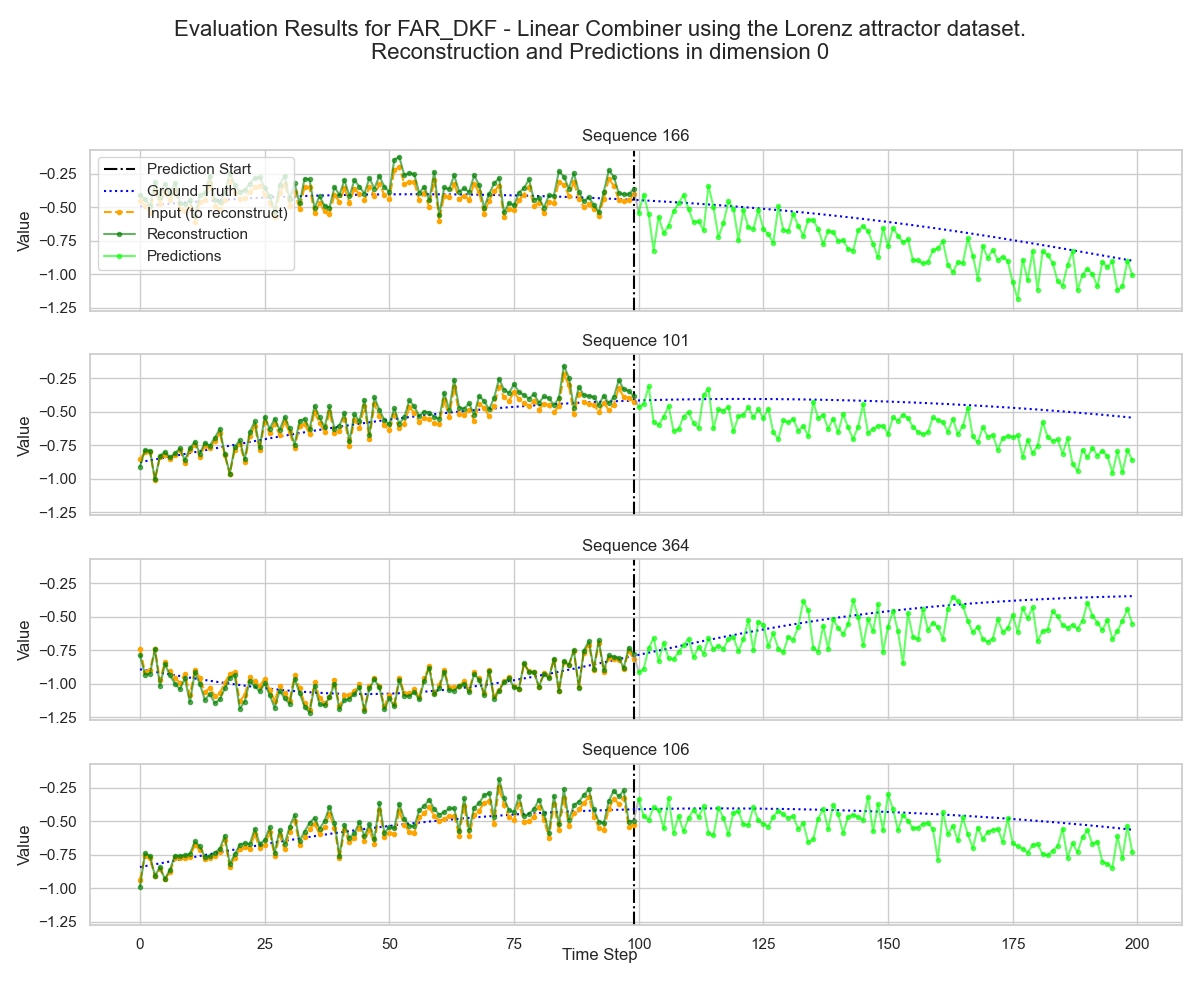
\includegraphics[width=1\textwidth]{./Images/Dataset_1/FAR_DKF_1_dim_0.png}
            \subcaption{Reconstruction and Prediction in the 1st dimension.}
            \label{fig:dataset_1_FAR_DKF_1_dim_0}
        \end{minipage}
        \hfill
        \begin{minipage}{0.31\textwidth}
            \centering
            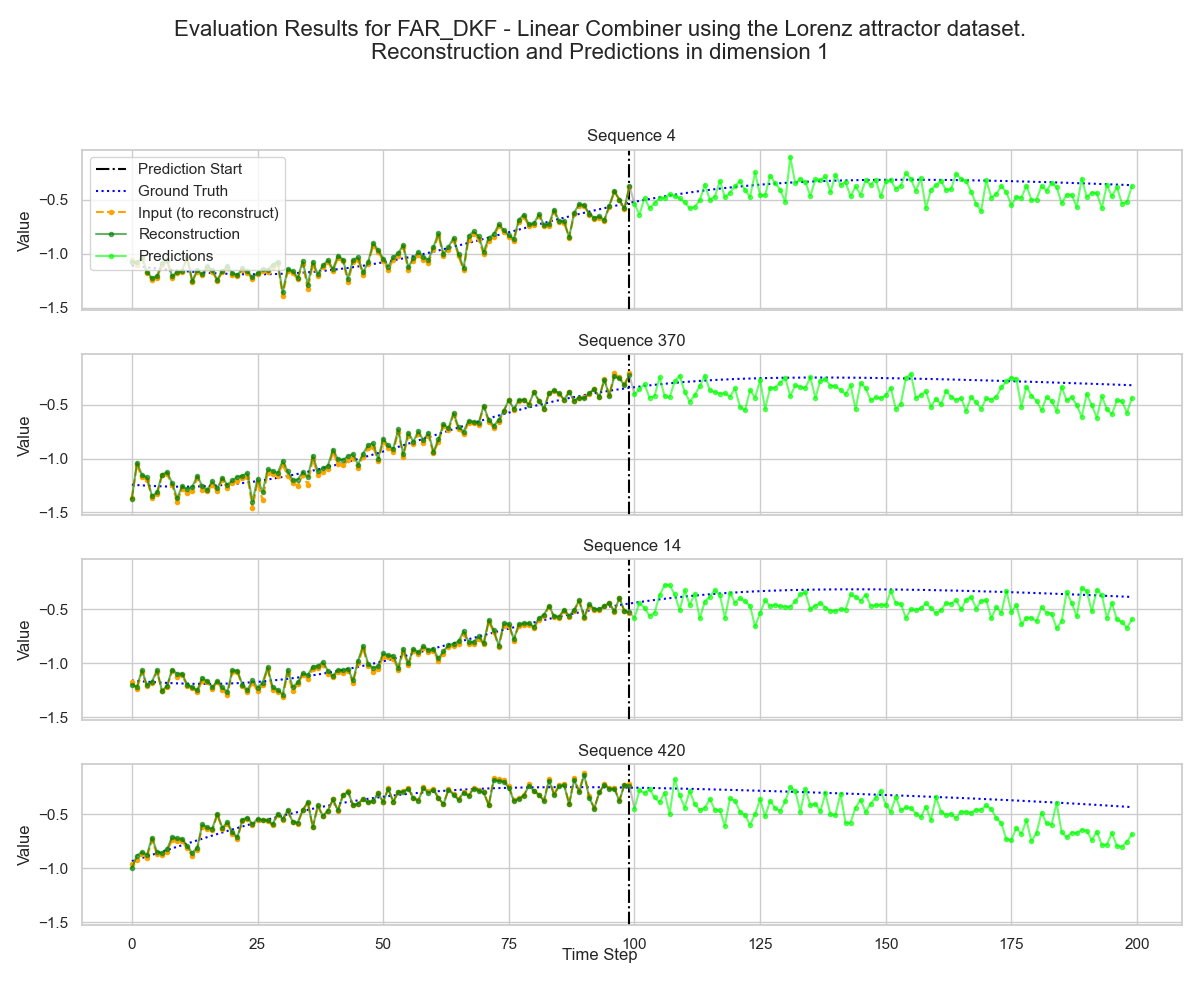
\includegraphics[width=1\textwidth]{./Images/Dataset_1/FAR_DKF_1_dim_1.png}
            \subcaption{Reconstruction and Prediction in the 2nd dimension.}
            \label{fig:dataset_1_FAR_DKF_1_dim_1}
        \end{minipage}
        \hfill
        \begin{minipage}{0.31\textwidth}
            \centering
            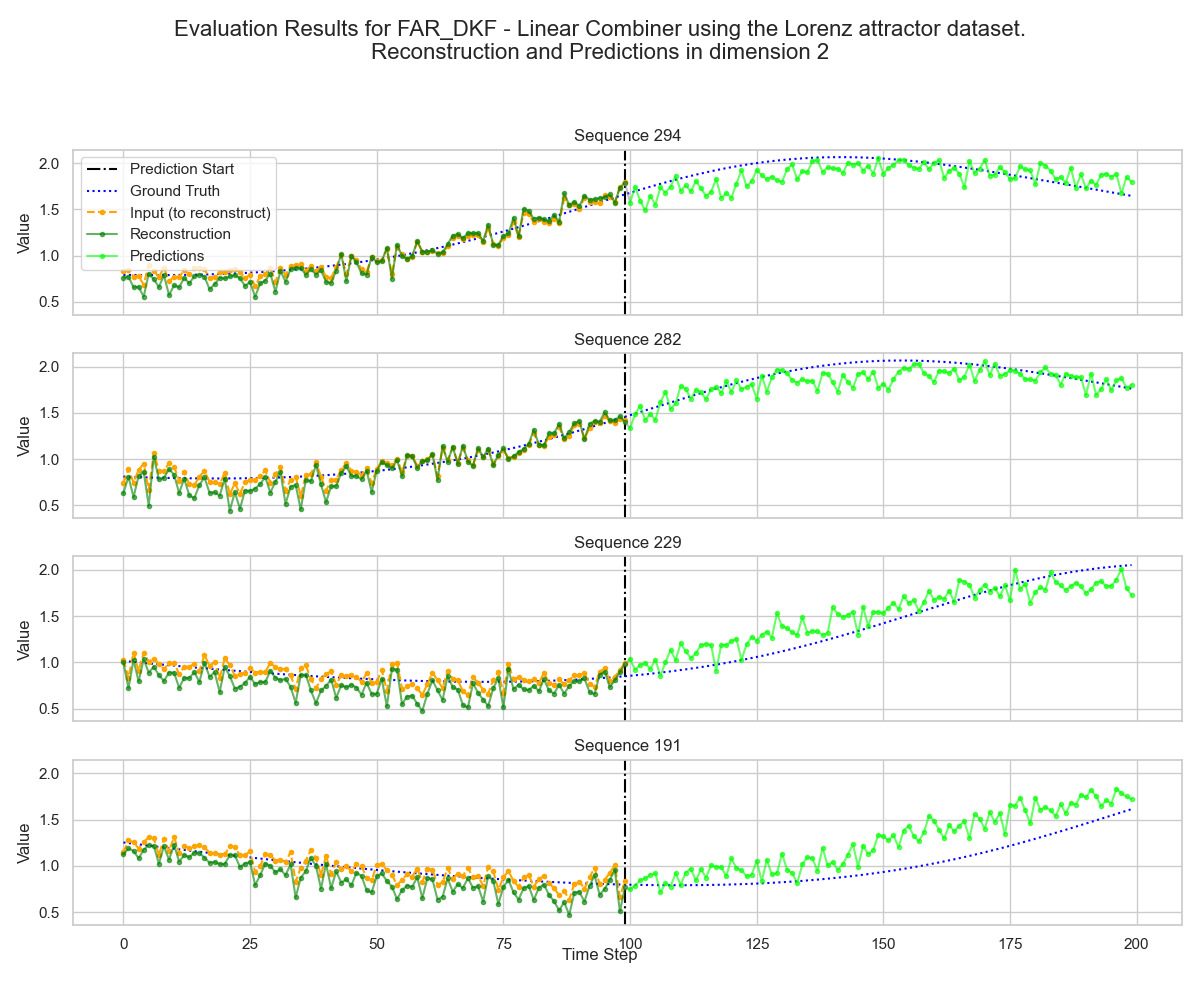
\includegraphics[width=1\textwidth]{./Images/Dataset_1/FAR_DKF_1_dim_2.png}
            \subcaption{Reconstruction and Prediction in the 3rd dimension.}
            \label{fig:dataset_1_FAR_DKF_1_dim_2}
        \end{minipage}
        \caption{Examples of Reconstruction and Prediction for the
        FAR DKF model.}
        \label{fig:dataset_1_FAR_DKF_1_all_dims}
    \end{figure}
    
    And Figure \ref{fig:dataset_1_BAR_DKF_1_all_dims} shows the results
    of the BAR DKF.
    
    \begin{figure}[ht!]
        \centering
        \begin{minipage}{0.31\textwidth}
            \centering
            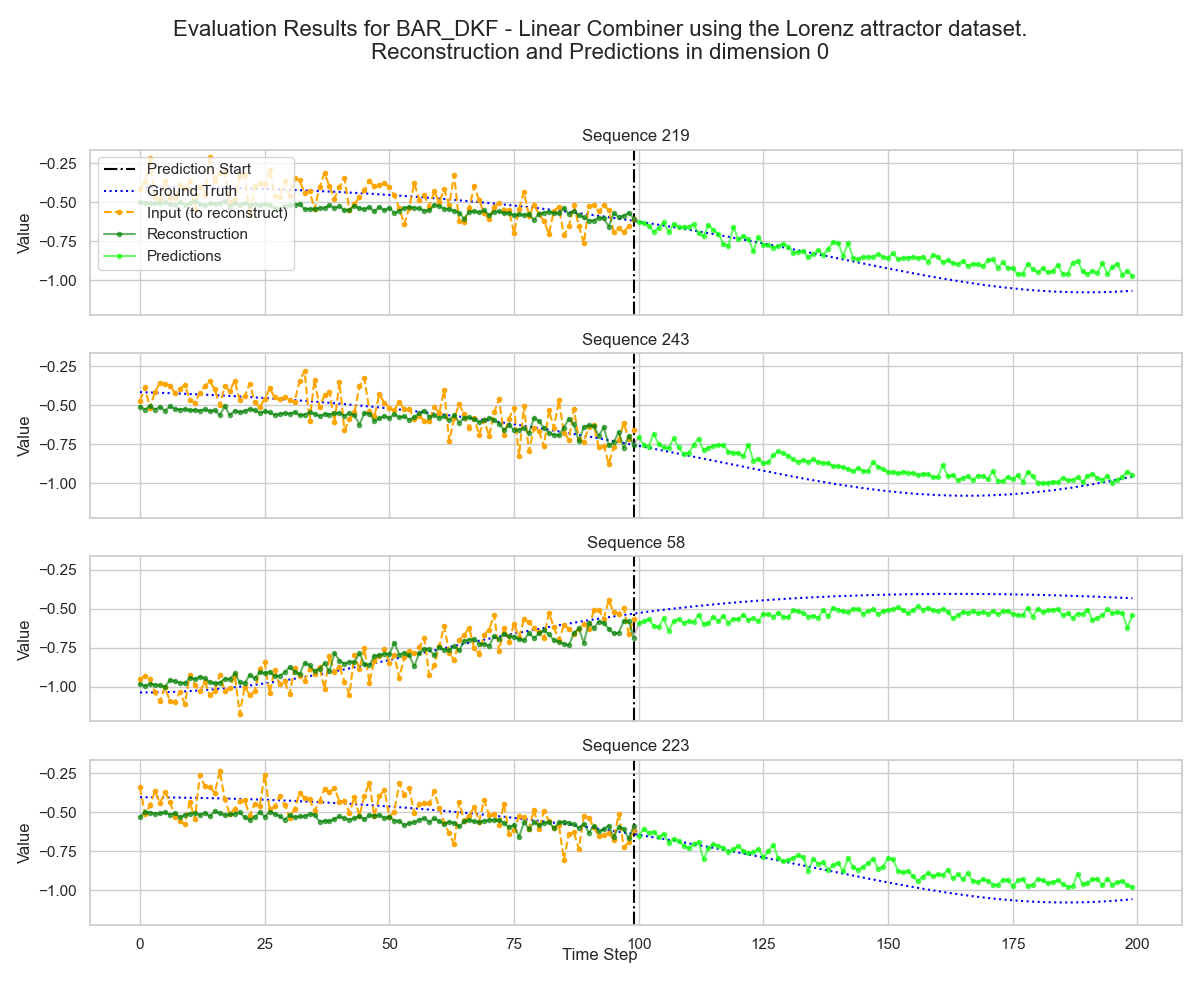
\includegraphics[width=1\textwidth]{./Images/Dataset_1/BAR_DKF_1_dim_0.png}
            \subcaption{Reconstruction and Prediction in the 1st dimension.}
            \label{fig:dataset_1_BAR_DKF_1_dim_0}
        \end{minipage}
        \hfill
        \begin{minipage}{0.31\textwidth}
            \centering
            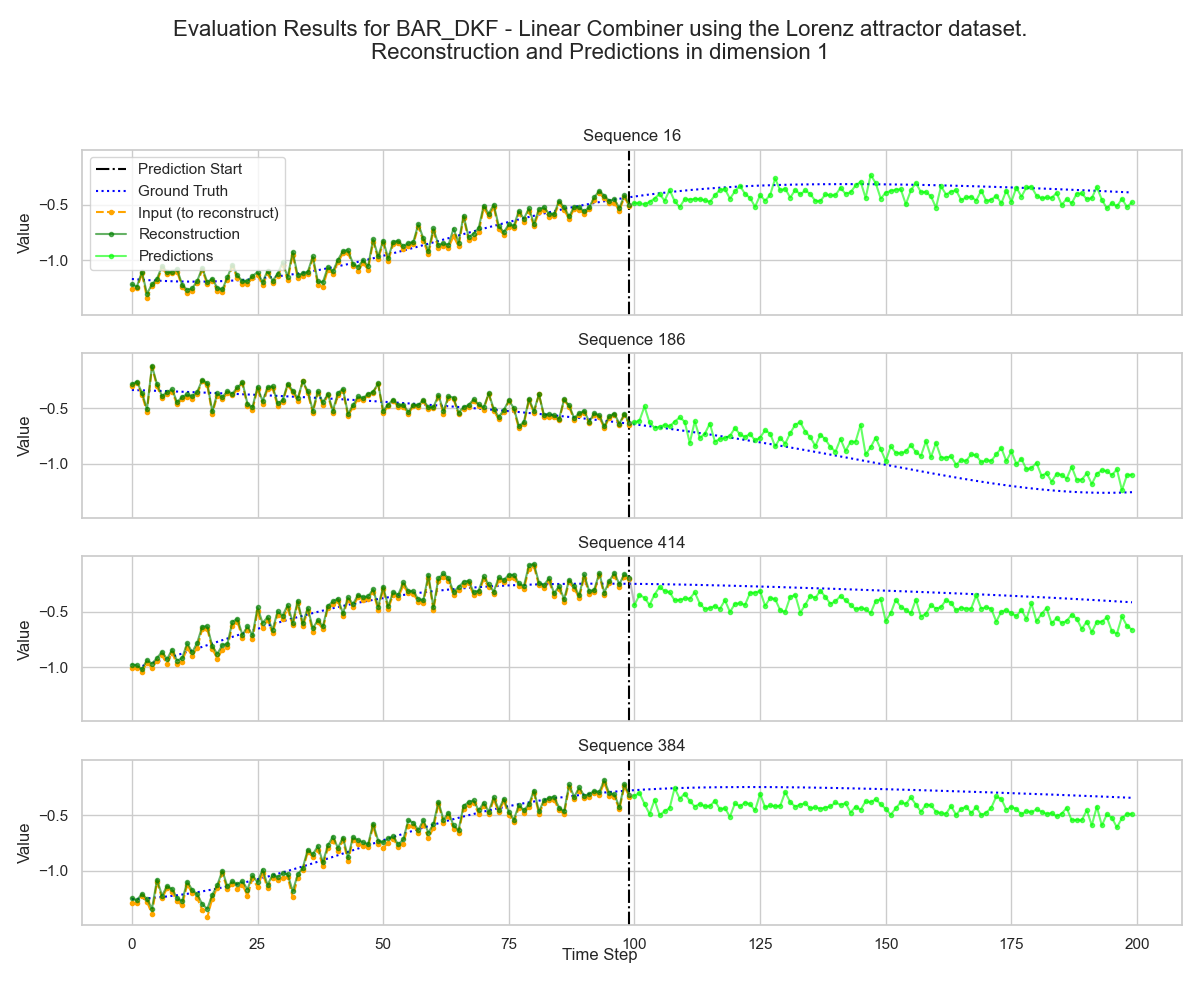
\includegraphics[width=1\textwidth]{./Images/Dataset_1/BAR_DKF_1_dim_1.png}
            \subcaption{Reconstruction and Prediction in the 2nd dimension.}
            \label{fig:dataset_1_BAR_DKF_1_dim_1}
        \end{minipage}
        \hfill
        \begin{minipage}{0.31\textwidth}
            \centering
            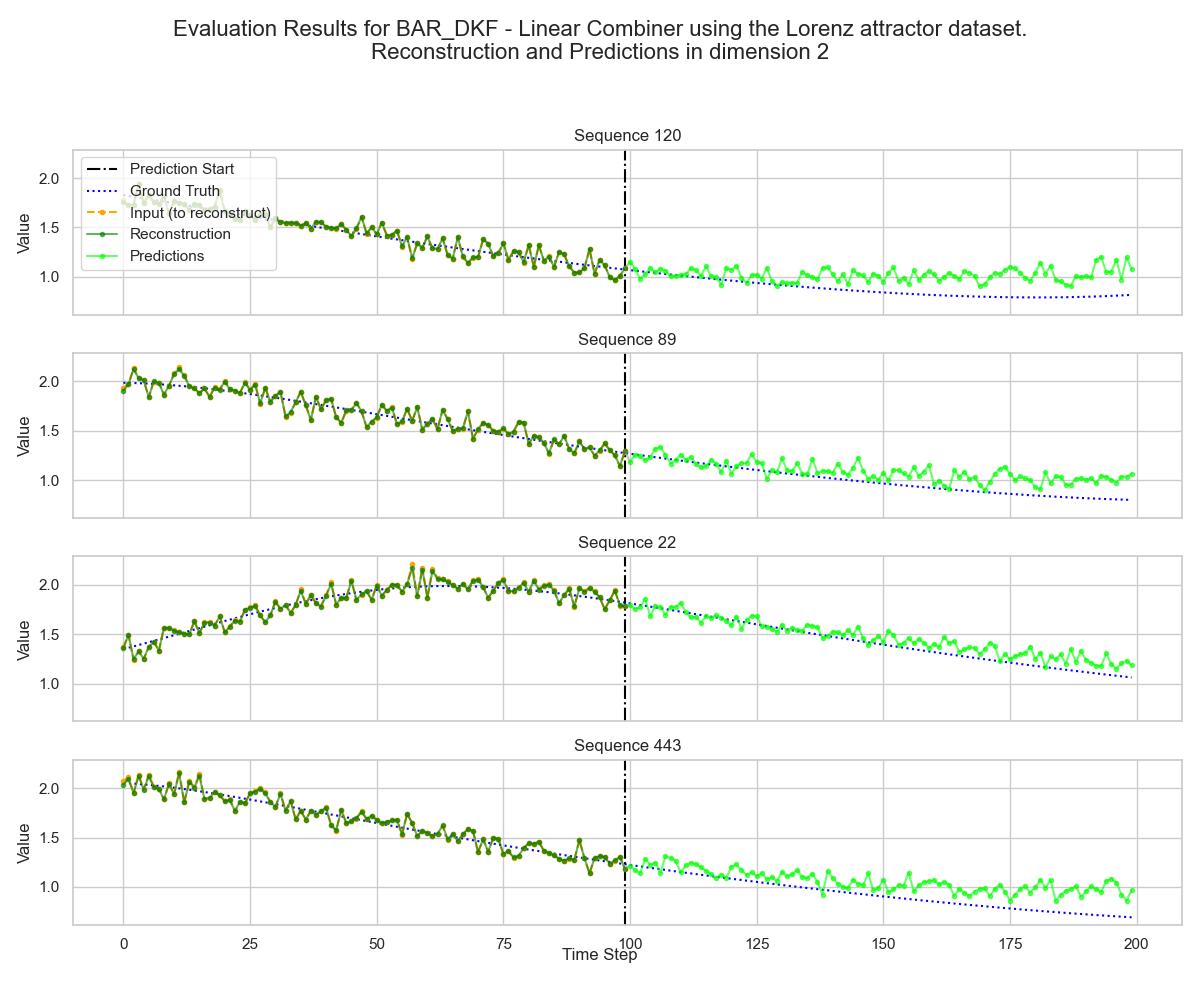
\includegraphics[width=1\textwidth]{./Images/Dataset_1/BAR_DKF_1_dim_2.png}
            \subcaption{Reconstruction and Prediction in the 3rd dimension.}
            \label{fig:dataset_1_BAR_DKF_1_dim_2}
        \end{minipage}
        \caption{Examples of Reconstruction and Prediction for the
        BAR DKF model.}
        \label{fig:dataset_1_BAR_DKF_1_all_dims}
    \end{figure}
    
    \FloatBarrier
    
    Figure \ref{fig:dataset_1_mse_comparison} below shows a
    comparison of the Mean Square Error for the reconstruction
    and the prediction tasks for each model. The MSE of the noise
    is plotted for reference.\\
    The three models have prediction errors of the same order: 0.0269
    for the AR DKF, 0.0309 for the FAR DKF and 0.0218 for the BAR DKF.
    The AR DKF and the BAR DKF reconstruct at the noise level. The FAR DKF
    reconstruction error (0.0092) is above it, i.e.\ worse than simply
    returning the noisy input.
    
    \begin{figure}[ht!]
        \centering
        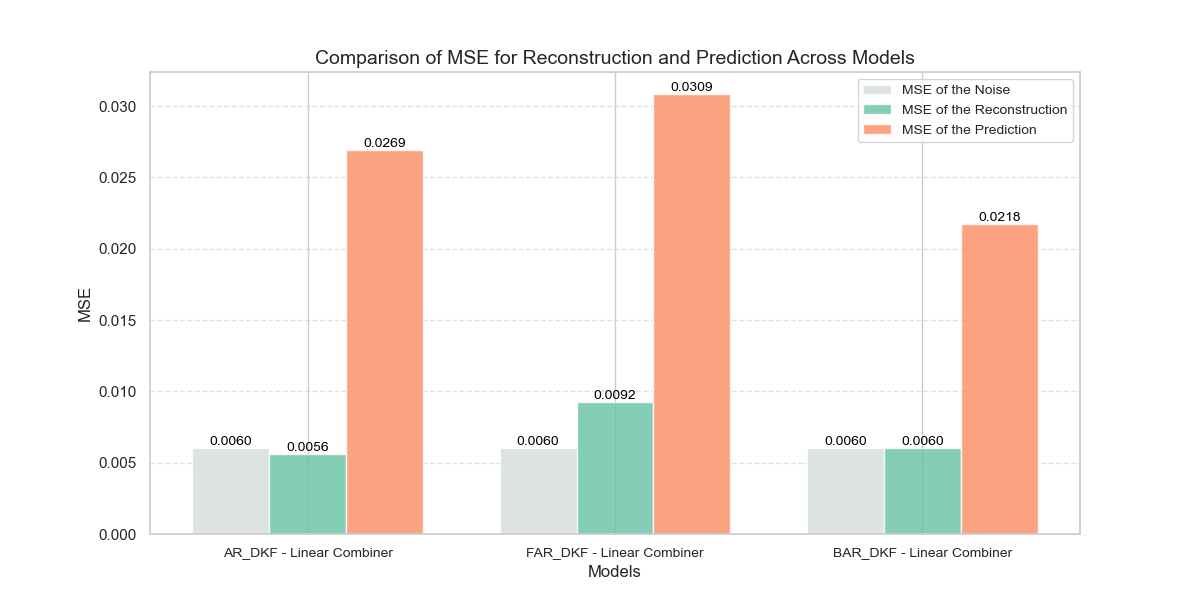
\includegraphics[width=0.75\textwidth]
        {./Images/Dataset_1/mse_comparison.png}
        \caption{Reconstruction and Prediction MSE Comparison for
        AR DKF, FAR DKF, and BAR DKF
        on dataset 1.}
        \label{fig:dataset_1_mse_comparison}
    \end{figure}
    
    Figure \ref{fig:dataset_1_mse_pred_comparison} below shows a
    comparison of the Mean Square Error for each predicted point
    for each model.\\
    As expected, the error grows with the forecasting horizon, since
    errors accumulate along the sampled path.
    
    \begin{figure}[ht!]
        \centering
        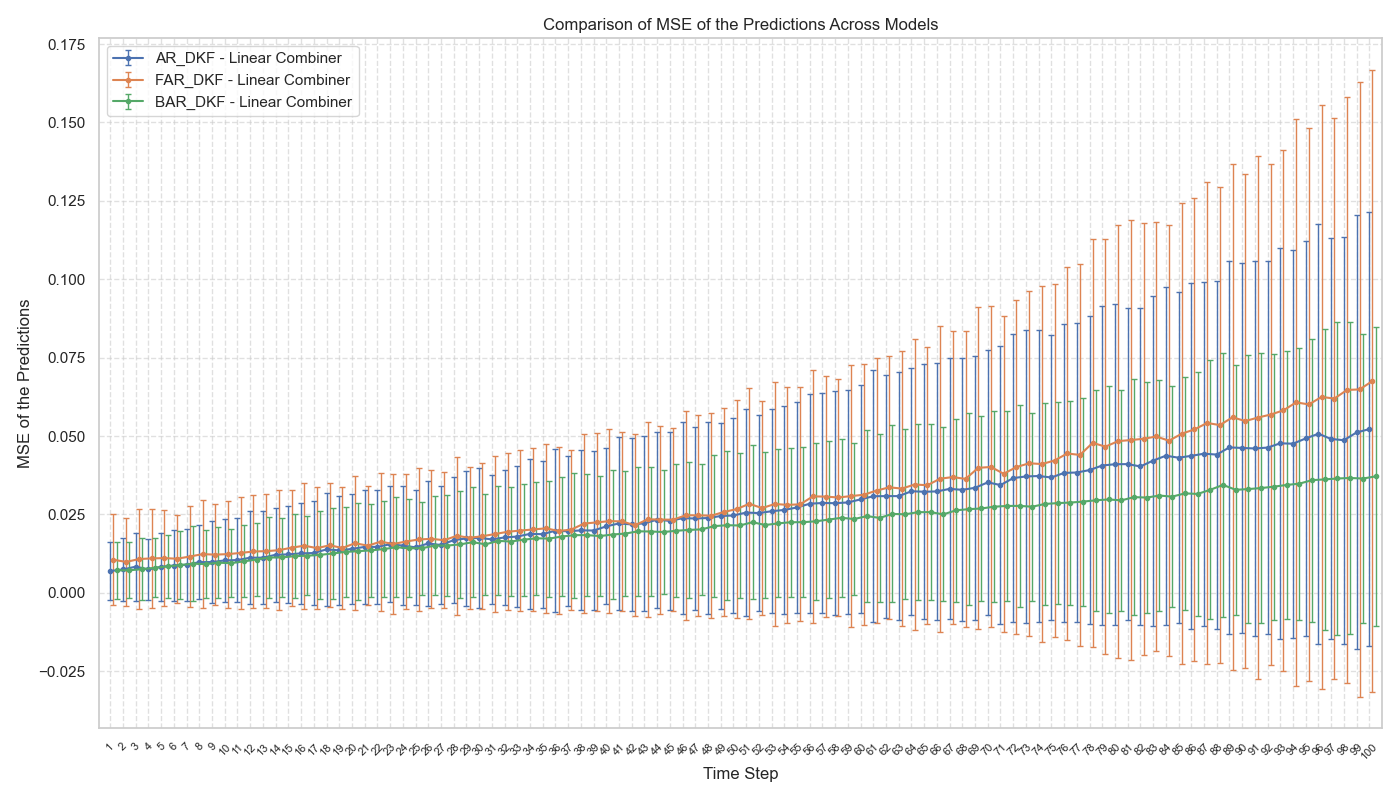
\includegraphics[width=1\textwidth]
        {./Images/Dataset_1/mse_pred_comparison.png}
        \caption{MSE Comparison for AR DKF, FAR DKF, and
        BAR DKF for each prediction points of test sequences of
        dataset 1.}
        \label{fig:dataset_1_mse_pred_comparison}
    \end{figure}
    %
    \FloatBarrier
    The same comparisons were done on the dataset 2 and 3.
    The results are shown below.
    %- - - - - - - - - - - - - - - - - - - - - - - - - - - - 
    \subsubsection*{Dataset 2}
    
    The dataset (\textit{before the addition of Gaussian noise}) is shown
    in figure \ref{fig:dataset_2_partial_data}.
    
    \begin{figure}[ht!]
        \centering
        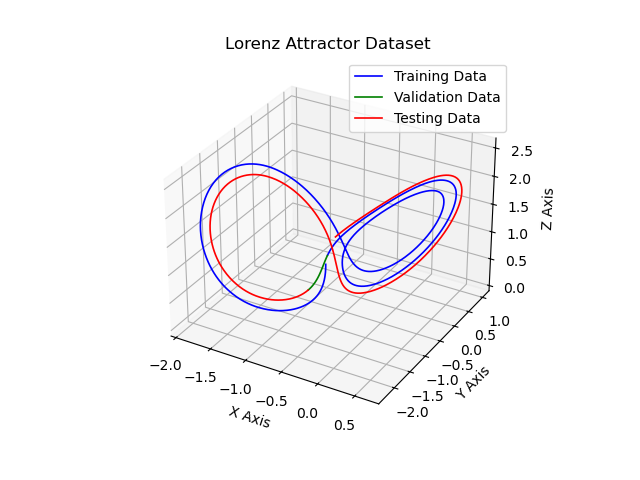
\includegraphics[width=0.75\textwidth]
        {./Images/Dataset_2/partial_data.png}
        \caption{Lorenz attractor - Range [8600, 10500] }
        \label{fig:dataset_2_partial_data}
    \end{figure}
    %
    \begin{figure}[ht!]
        \centering
        \begin{minipage}{0.31\textwidth}
            \centering
            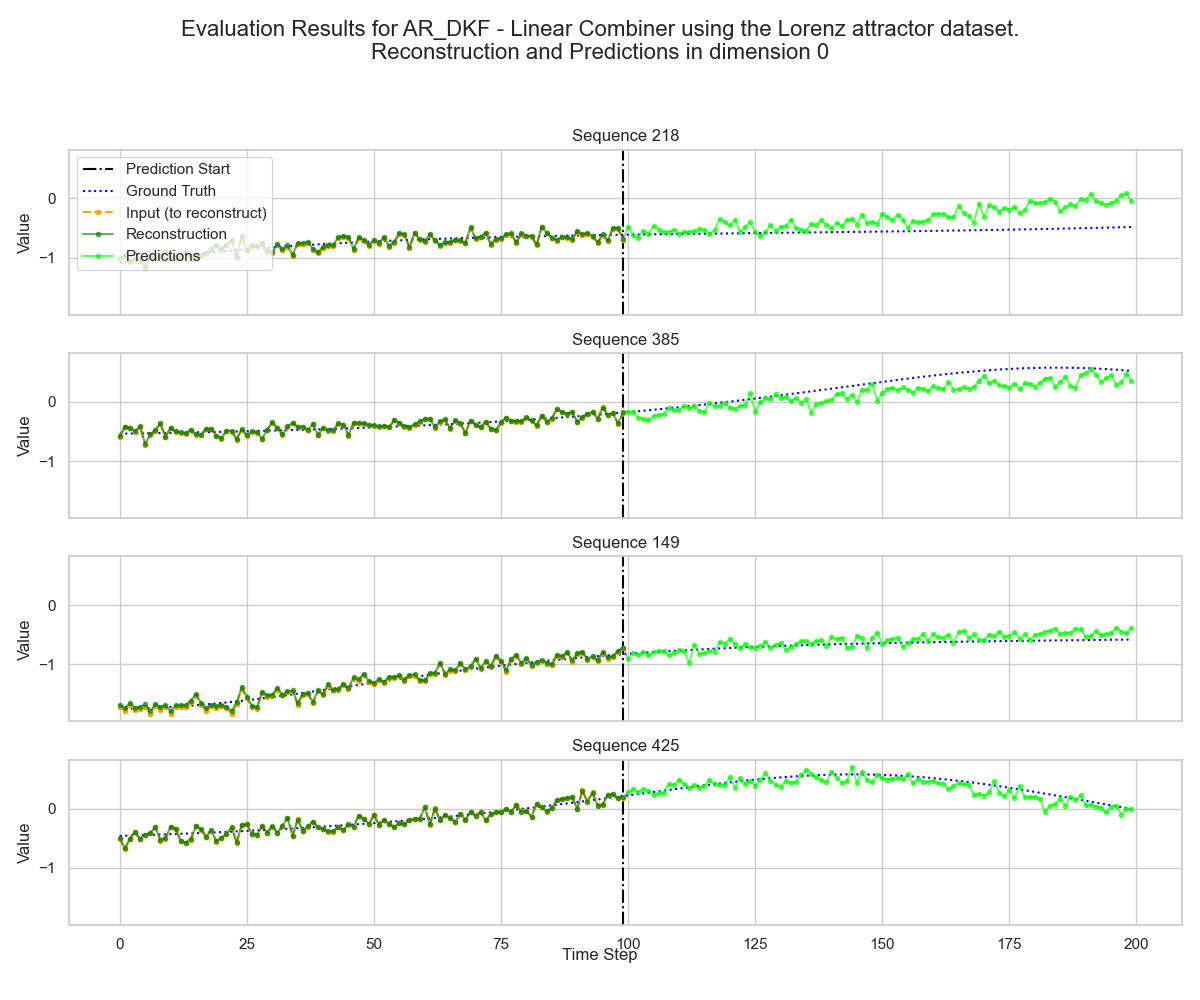
\includegraphics[width=1\textwidth]{./Images/Dataset_2/AR_DKF_1_dim_0.png}
            \subcaption{Reconstruction and Prediction in the 1st dimension.}
            \label{fig:dataset_2_AR_DKF_1_dim_0}
        \end{minipage}
        \hfill
        \begin{minipage}{0.31\textwidth}
            \centering
            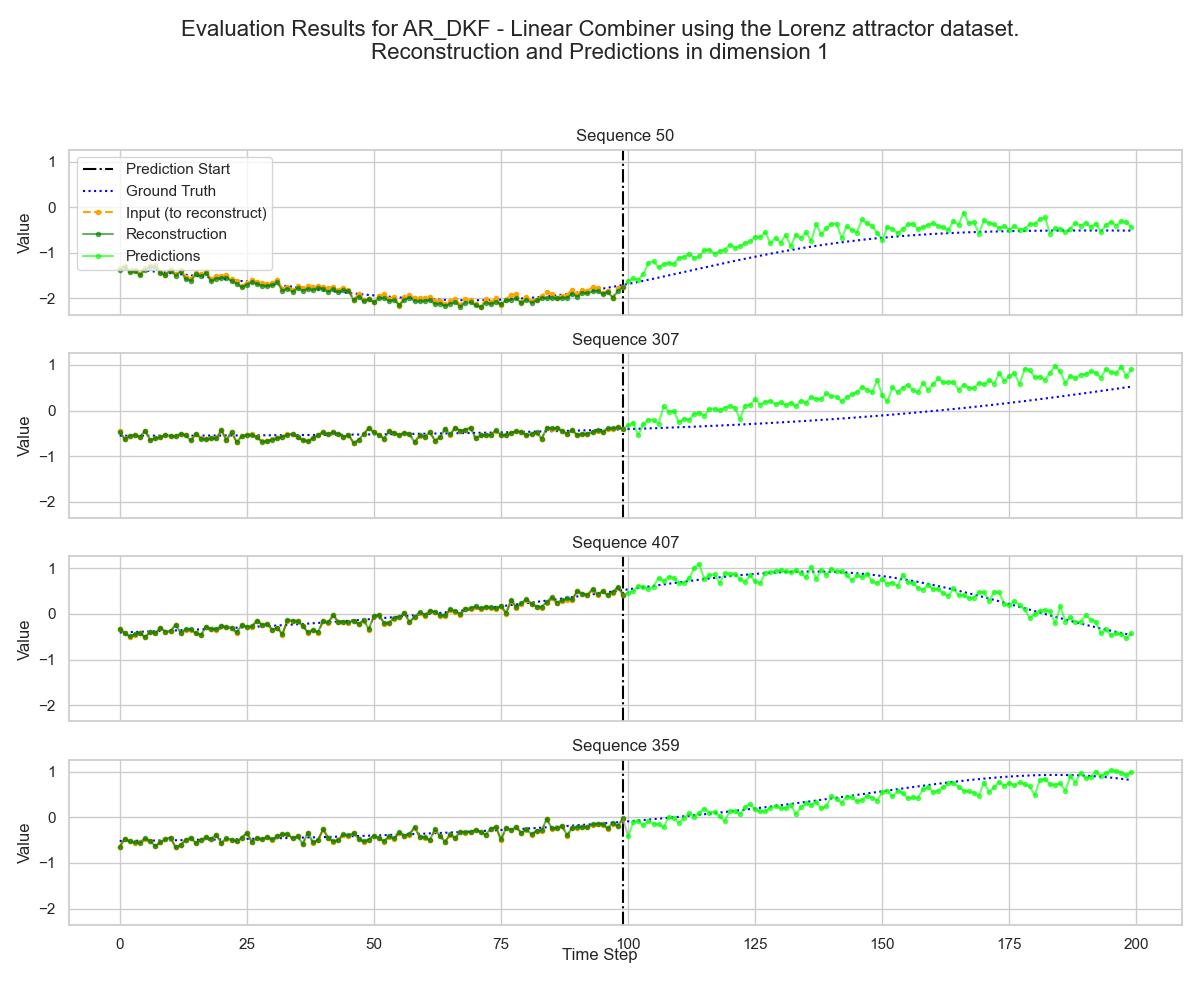
\includegraphics[width=1\textwidth]{./Images/Dataset_2/AR_DKF_1_dim_1.png}
            \subcaption{Reconstruction and Prediction in the 2nd dimension.}
            \label{fig:dataset_2_AR_DKF_1_dim_1}
        \end{minipage}
        \hfill
        \begin{minipage}{0.31\textwidth}
            \centering
            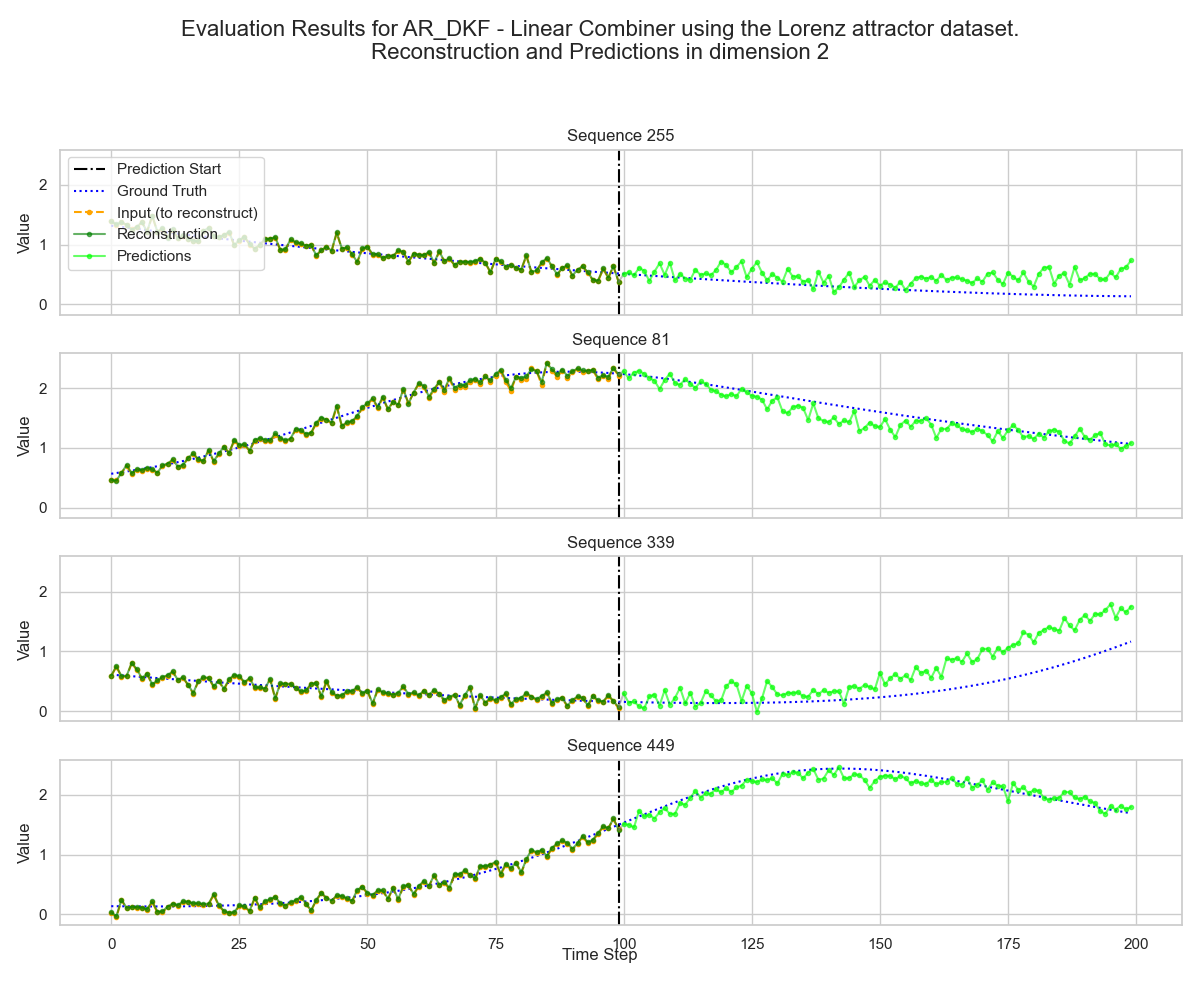
\includegraphics[width=1\textwidth]{./Images/Dataset_2/AR_DKF_1_dim_2.png}
            \subcaption{Reconstruction and Prediction in the 3rd dimension.}
            \label{fig:dataset_2_AR_DKF_1_dim_2}
        \end{minipage}
        \caption{Examples of Reconstruction and Prediction for the
        AR DKF model.}
        \label{fig:dataset_2_AR_DKF_1_all_dims}
    \end{figure}
    
    \begin{figure}[ht!]
        \centering
        \begin{minipage}{0.31\textwidth}
            \centering
            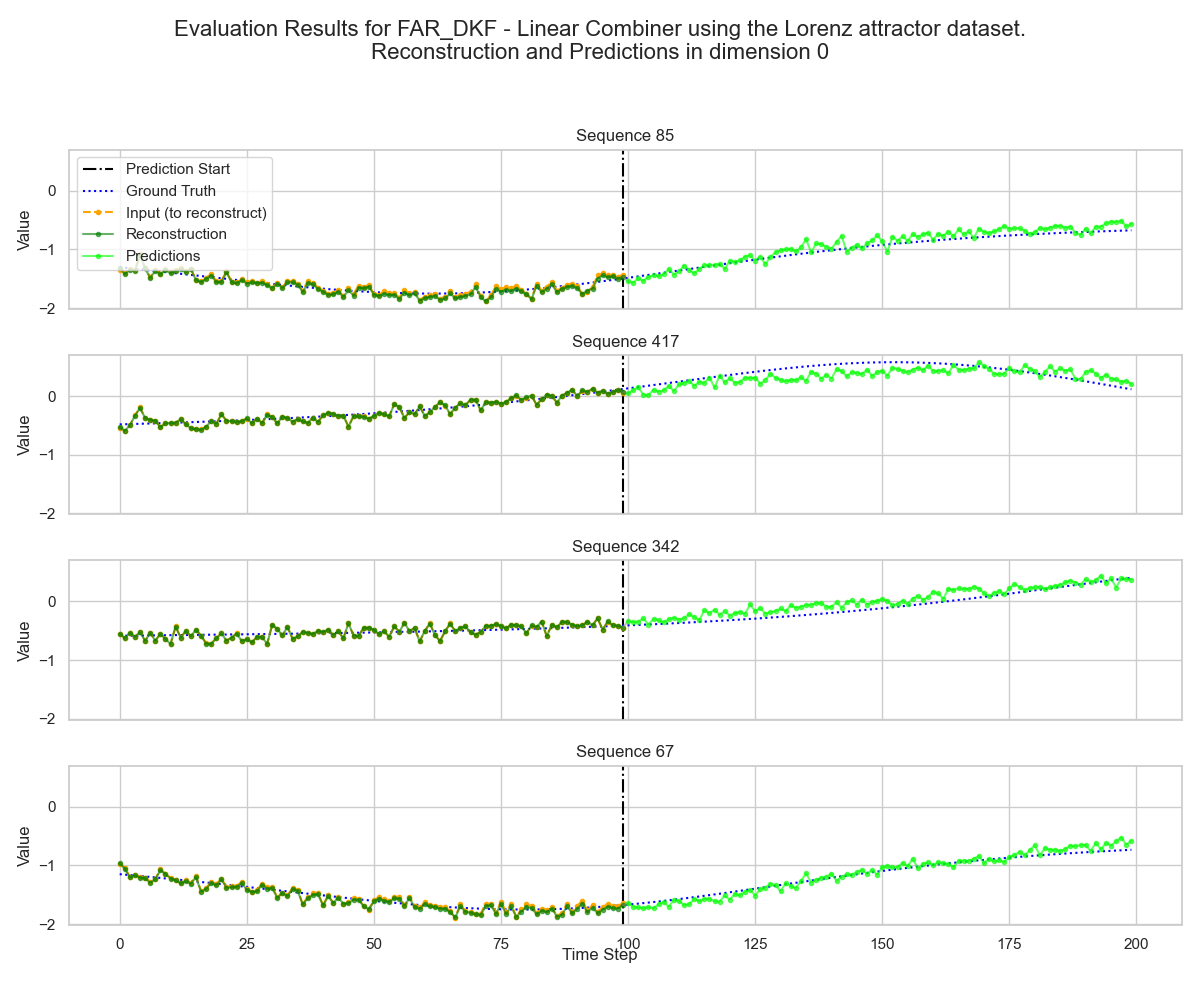
\includegraphics[width=1\textwidth]{./Images/Dataset_2/FAR_DKF_1_dim_0.png}
            \subcaption{Reconstruction and Prediction in the 1st dimension.}
            \label{fig:dataset_2_FAR_DKF_1_dim_0}
        \end{minipage}
        \hfill
        \begin{minipage}{0.31\textwidth}
            \centering
            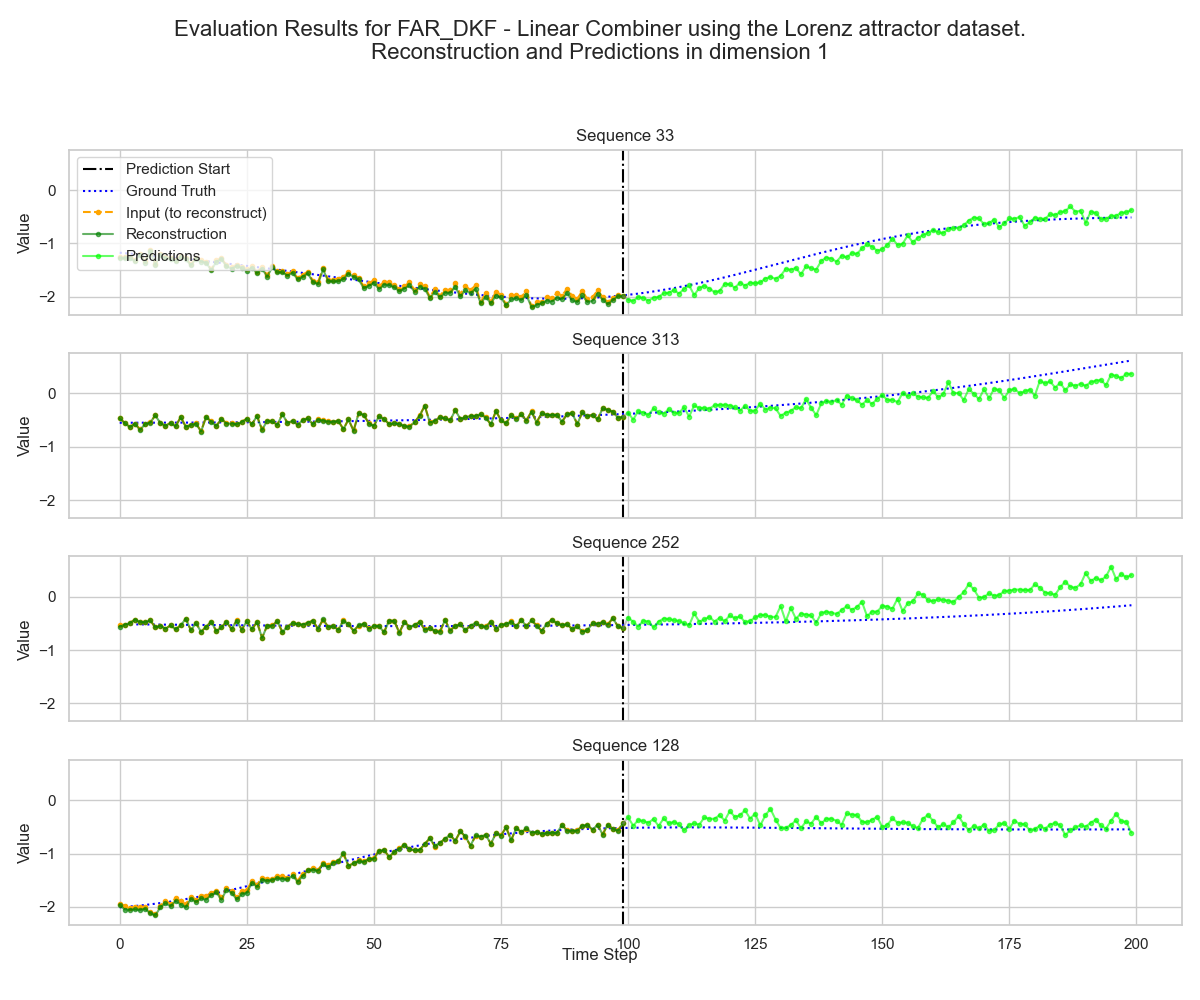
\includegraphics[width=1\textwidth]{./Images/Dataset_2/FAR_DKF_1_dim_1.png}
            \subcaption{Reconstruction and Prediction in the 2nd dimension.}
            \label{fig:dataset_2_FAR_DKF_1_dim_1}
        \end{minipage}
        \hfill
        \begin{minipage}{0.31\textwidth}
            \centering
            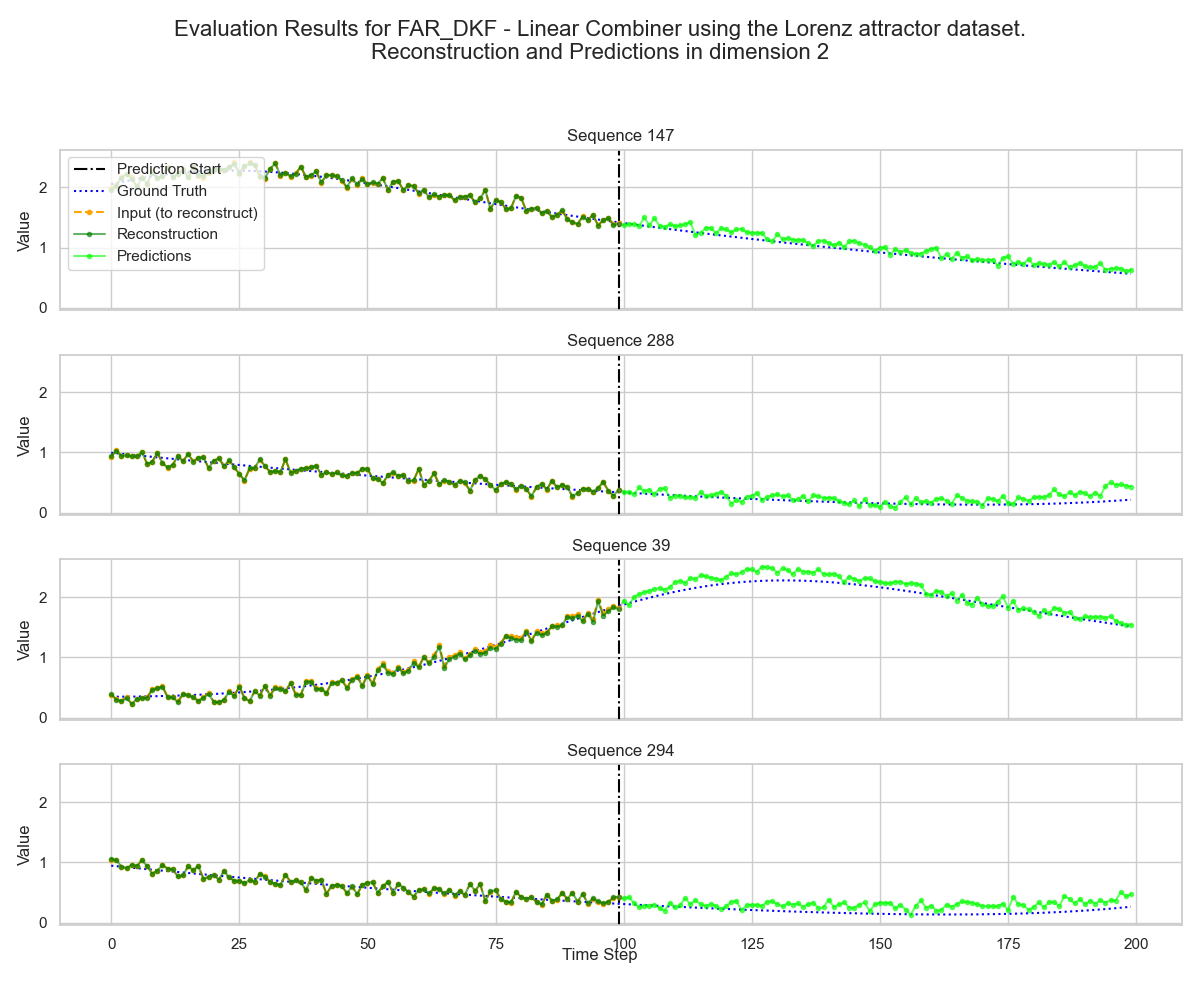
\includegraphics[width=1\textwidth]{./Images/Dataset_2/FAR_DKF_1_dim_2.png}
            \subcaption{Reconstruction and Prediction in the 3rd dimension.}
            \label{fig:dataset_2_FAR_DKF_1_dim_2}
        \end{minipage}
        \caption{Examples of Reconstruction and Prediction for the
        FAR DKF model.}
        \label{fig:dataset_2_FAR_DKF_1_all_dims}
    \end{figure}
    
    \begin{figure}[ht!]
        \centering
        \begin{minipage}{0.31\textwidth}
            \centering
            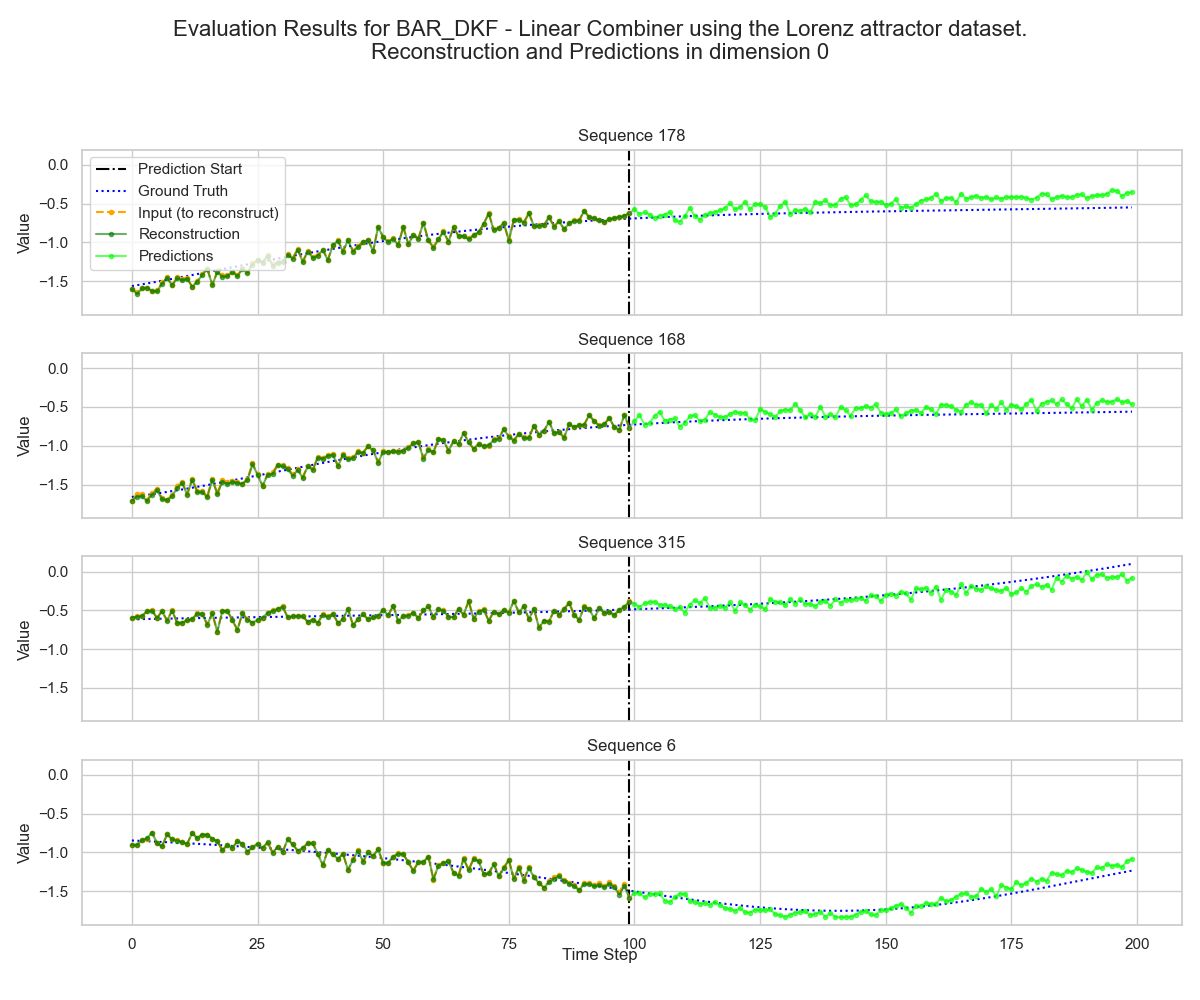
\includegraphics[width=1\textwidth]{./Images/Dataset_2/BAR_DKF_1_dim_0.png}
            \subcaption{Reconstruction and Prediction in the 1st dimension.}
            \label{fig:dataset_2_BAR_DKF_1_dim_0}
        \end{minipage}
        \hfill
        \begin{minipage}{0.31\textwidth}
            \centering
            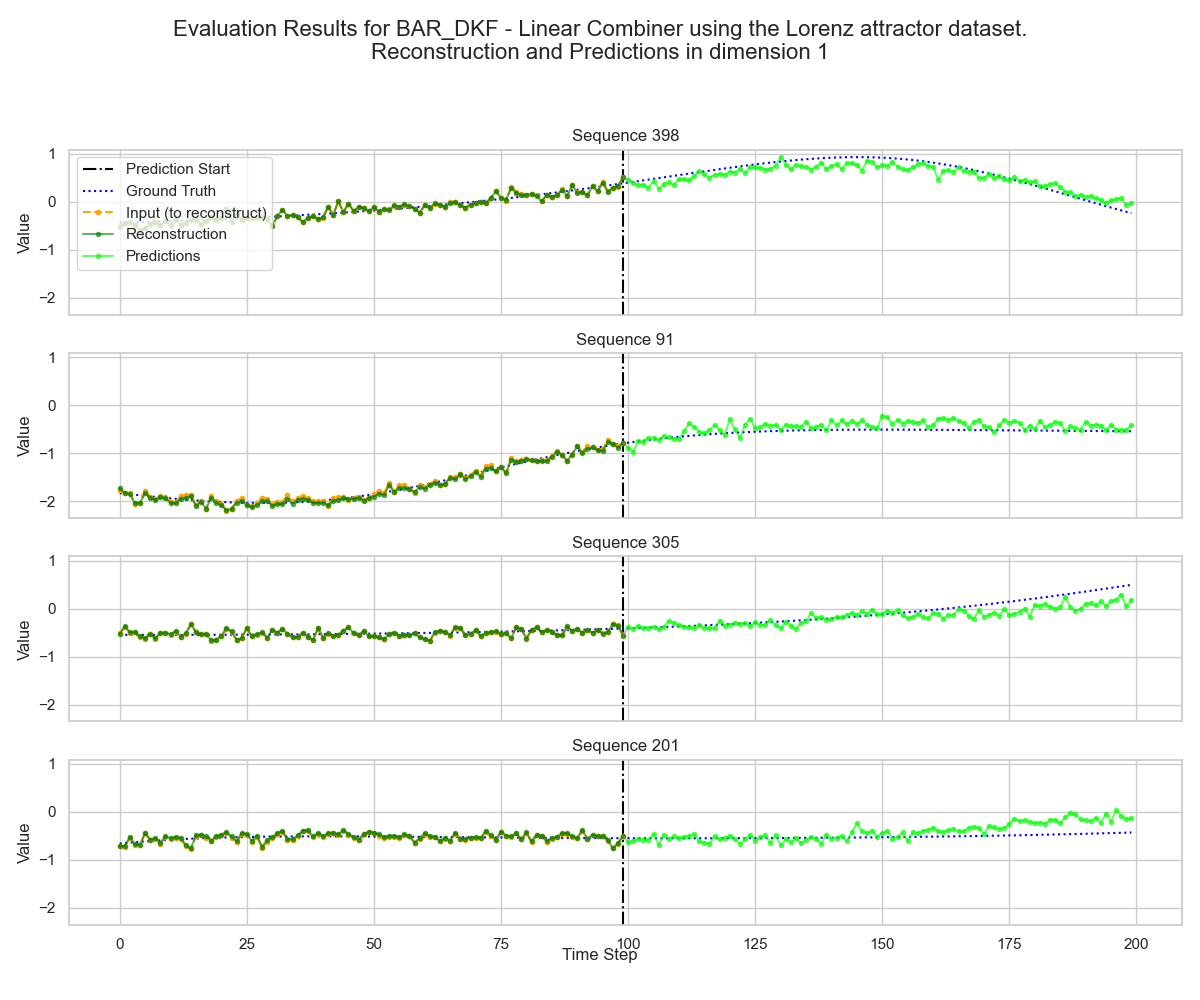
\includegraphics[width=1\textwidth]{./Images/Dataset_2/BAR_DKF_1_dim_1.png}
            \subcaption{Reconstruction and Prediction in the 2nd dimension.}
            \label{fig:dataset_2_BAR_DKF_1_dim_1}
        \end{minipage}
        \hfill
        \begin{minipage}{0.31\textwidth}
            \centering
            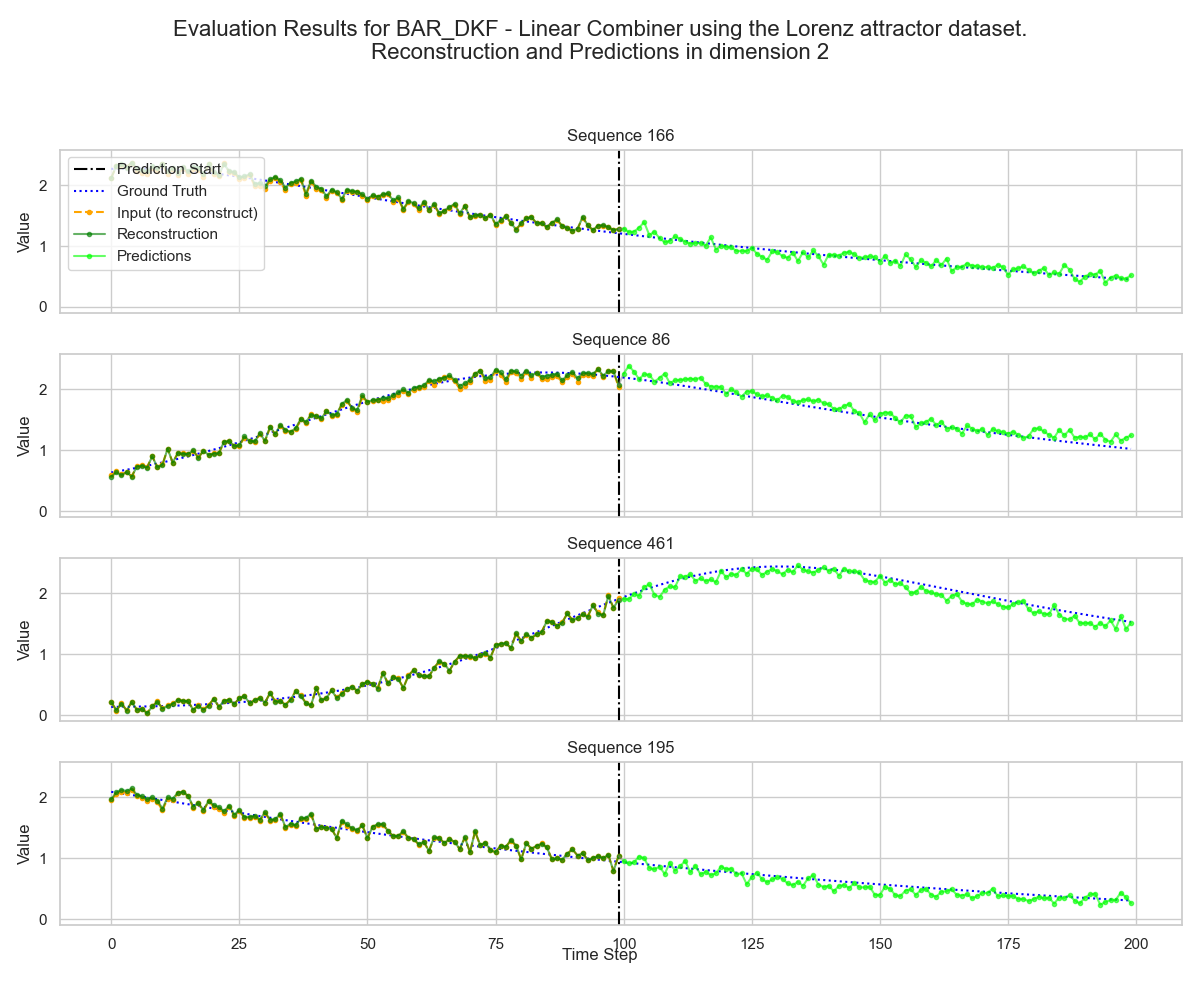
\includegraphics[width=1\textwidth]{./Images/Dataset_2/BAR_DKF_1_dim_2.png}
            \subcaption{Reconstruction and Prediction in the 3rd dimension.}
            \label{fig:dataset_2_BAR_DKF_1_dim_2}
        \end{minipage}
        \caption{Examples of Reconstruction and Prediction for the
        BAR DKF model.}
        \label{fig:dataset_2_BAR_DKF_1_all_dims}
    \end{figure}
    
    \begin{figure}[ht!]
        \centering
        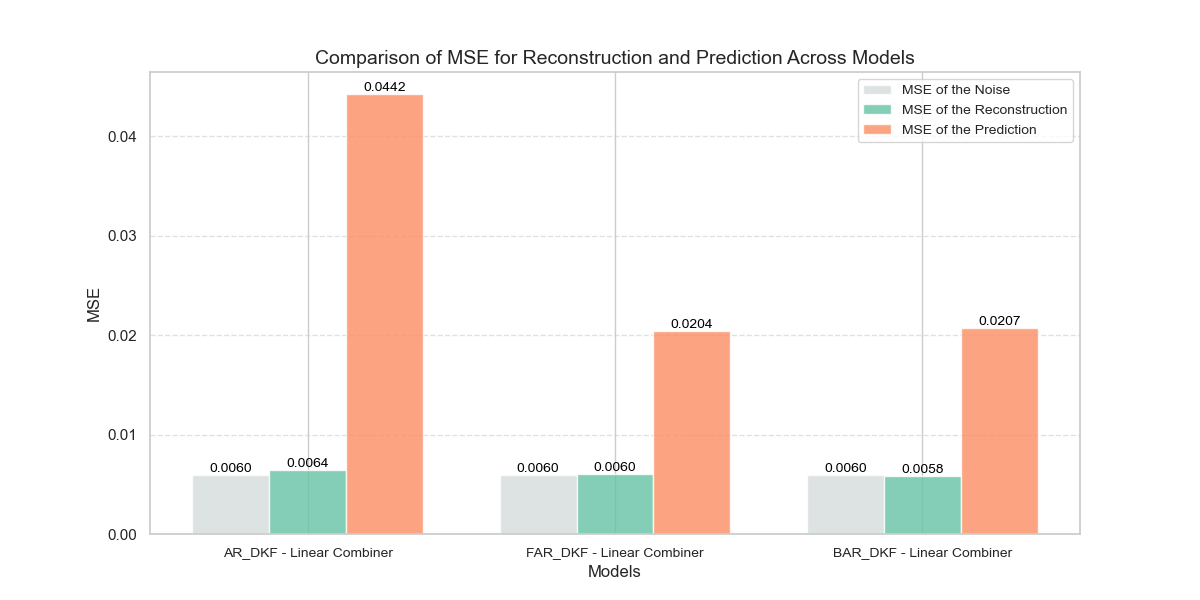
\includegraphics[width=0.75\textwidth]
        {./Images/Dataset_2/mse_comparison.png}
        \caption{Reconstruction and Prediction MSE Comparison for
        AR DKF, FAR DKF, and BAR DKF
        on dataset 2.}
        \label{fig:dataset_2_mse_comparison}
    \end{figure}
    
    \begin{figure}[ht!]
        \centering
        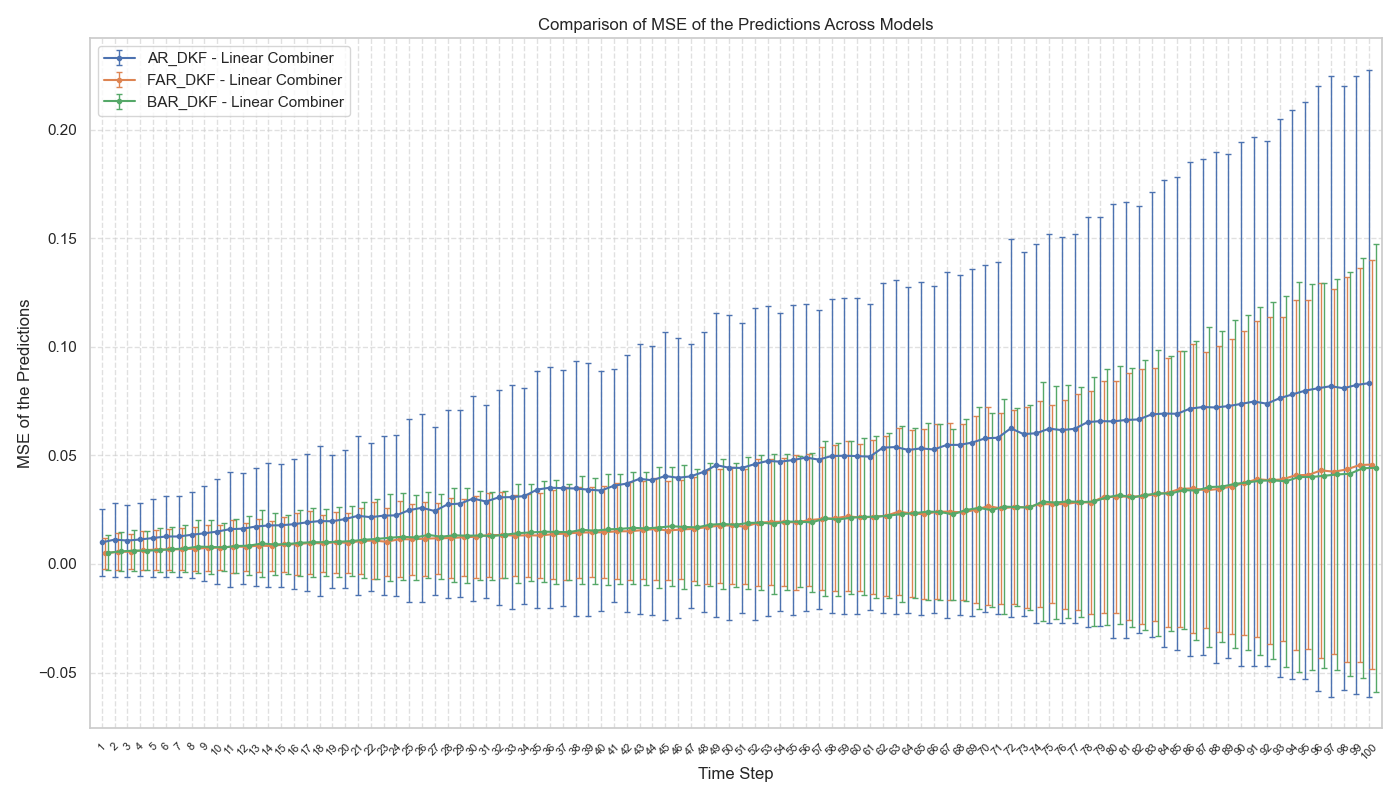
\includegraphics[width=1\textwidth]
        {./Images/Dataset_2/mse_pred_comparison.png}
        \caption{MSE Comparison for AR DKF, FAR DKF, and
        BAR DKF for each prediction points of test sequences of
        dataset 2.}
        \label{fig:dataset_2_mse_pred_comparison}
    \end{figure}
    %- - - - - - - - - - - - - - - - - - - - - - - - - - - - 
    \FloatBarrier
    \subsubsection*{Dataset 3}
    
    The dataset (\textit{before the addition of Gaussian noise}) is shown
    in figure \ref{fig:dataset_3_partial_data} below.\\
    
    \begin{figure}[ht!]
        \centering
        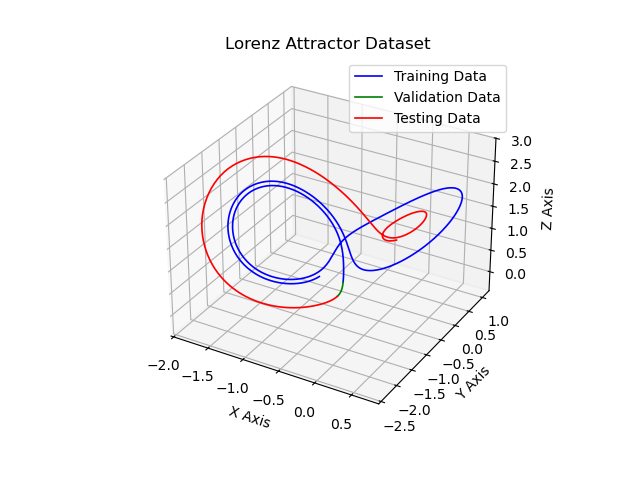
\includegraphics[width=0.75\textwidth]
        {./Images/Dataset_3/partial_data.png}
        \caption{Lorenz attractor - Range [11000, 13000] }
        \label{fig:dataset_3_partial_data}
    \end{figure}
    
    \begin{figure}[ht!]
        \centering
        \begin{minipage}{0.31\textwidth}
            \centering
            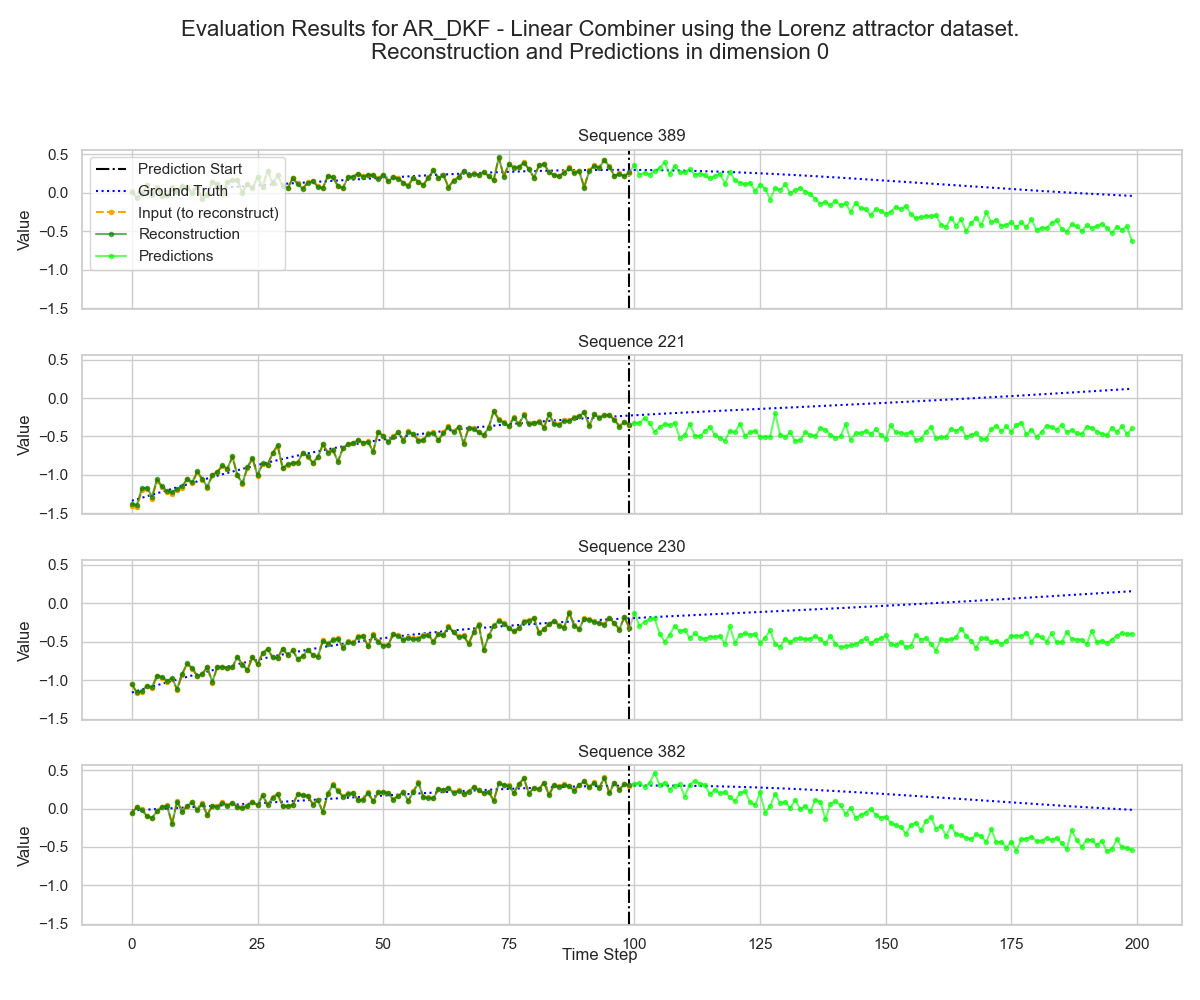
\includegraphics[width=1\textwidth]{./Images/Dataset_3/AR_DKF_1_dim_0.png}
            \subcaption{Reconstruction and Prediction in the 1st dimension.}
            \label{fig:dataset_3_AR_DKF_1_dim_0}
        \end{minipage}
        \hfill
        \begin{minipage}{0.31\textwidth}
            \centering
            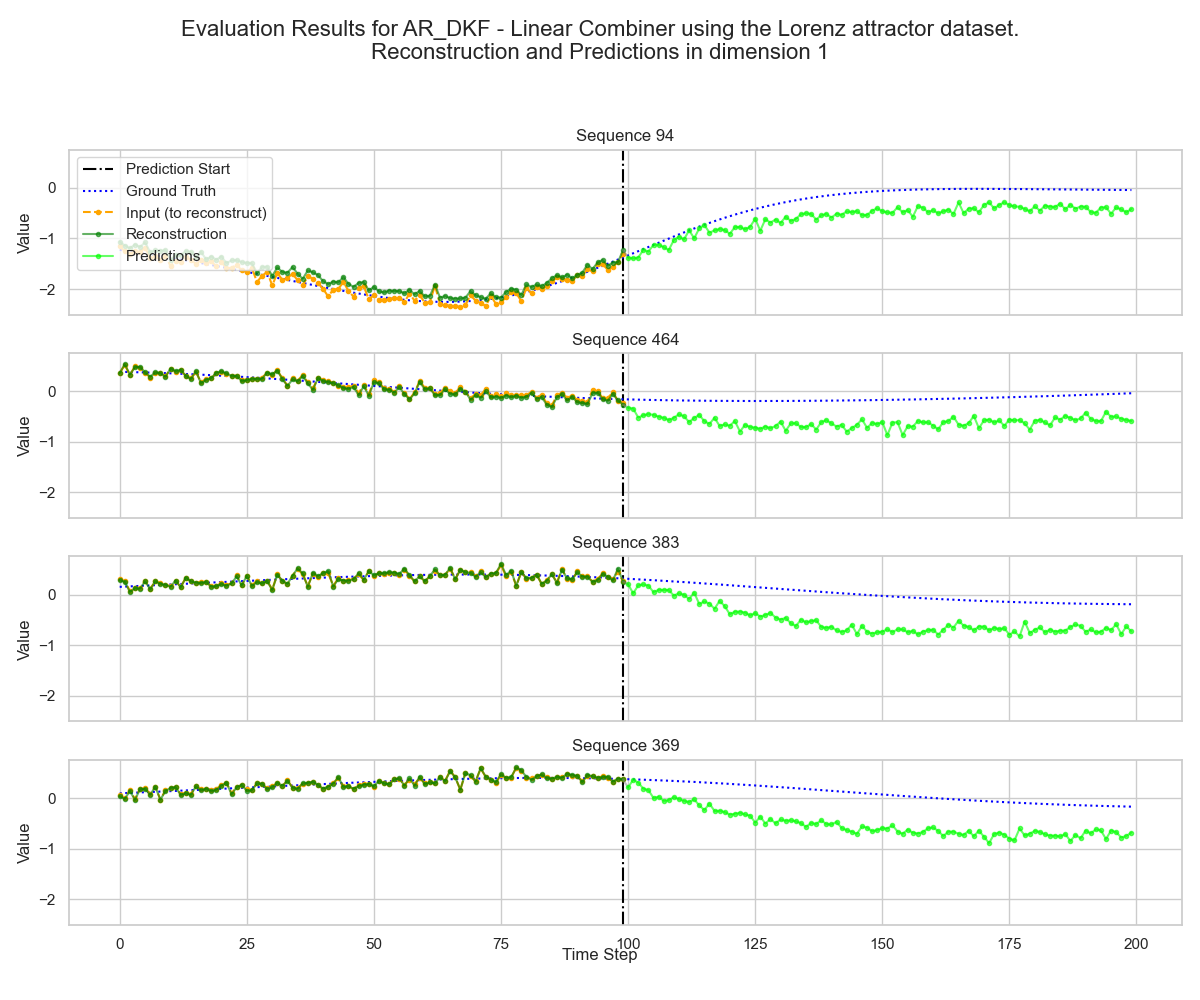
\includegraphics[width=1\textwidth]{./Images/Dataset_3/AR_DKF_1_dim_1.png}
            \subcaption{Reconstruction and Prediction in the 2nd dimension.}
            \label{fig:dataset_3_AR_DKF_1_dim_1}
        \end{minipage}
        \hfill
        \begin{minipage}{0.31\textwidth}
            \centering
            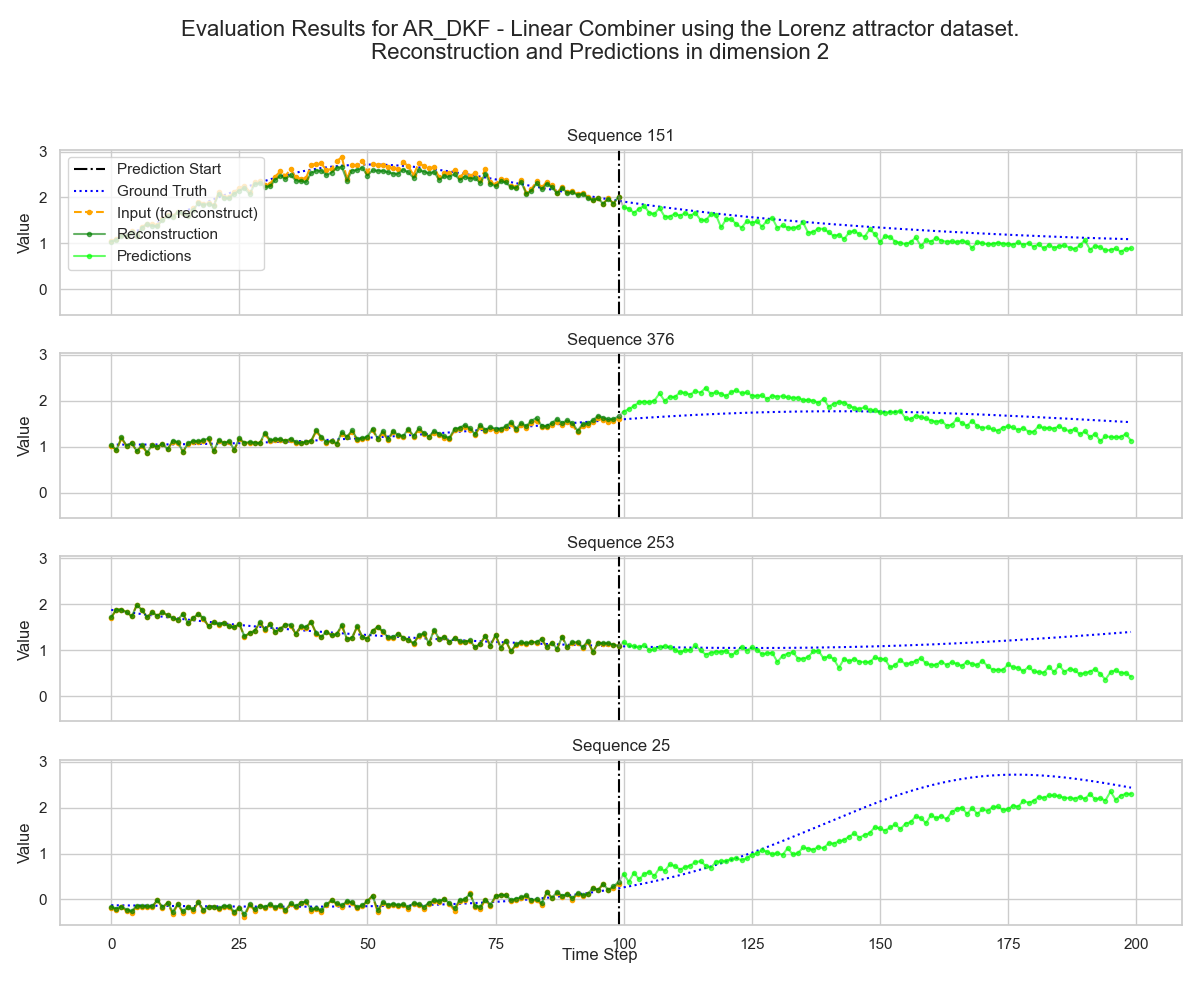
\includegraphics[width=1\textwidth]{./Images/Dataset_3/AR_DKF_1_dim_2.png}
            \subcaption{Reconstruction and Prediction in the 3rd dimension.}
            \label{fig:dataset_3_AR_DKF_1_dim_2}
        \end{minipage}
        \caption{Examples of Reconstruction and Prediction for the
        AR DKF model.}
        \label{fig:dataset_3_AR_DKF_1_all_dims}
    \end{figure}
    
    \begin{figure}[ht!]
        \centering
        \begin{minipage}{0.31\textwidth}
            \centering
            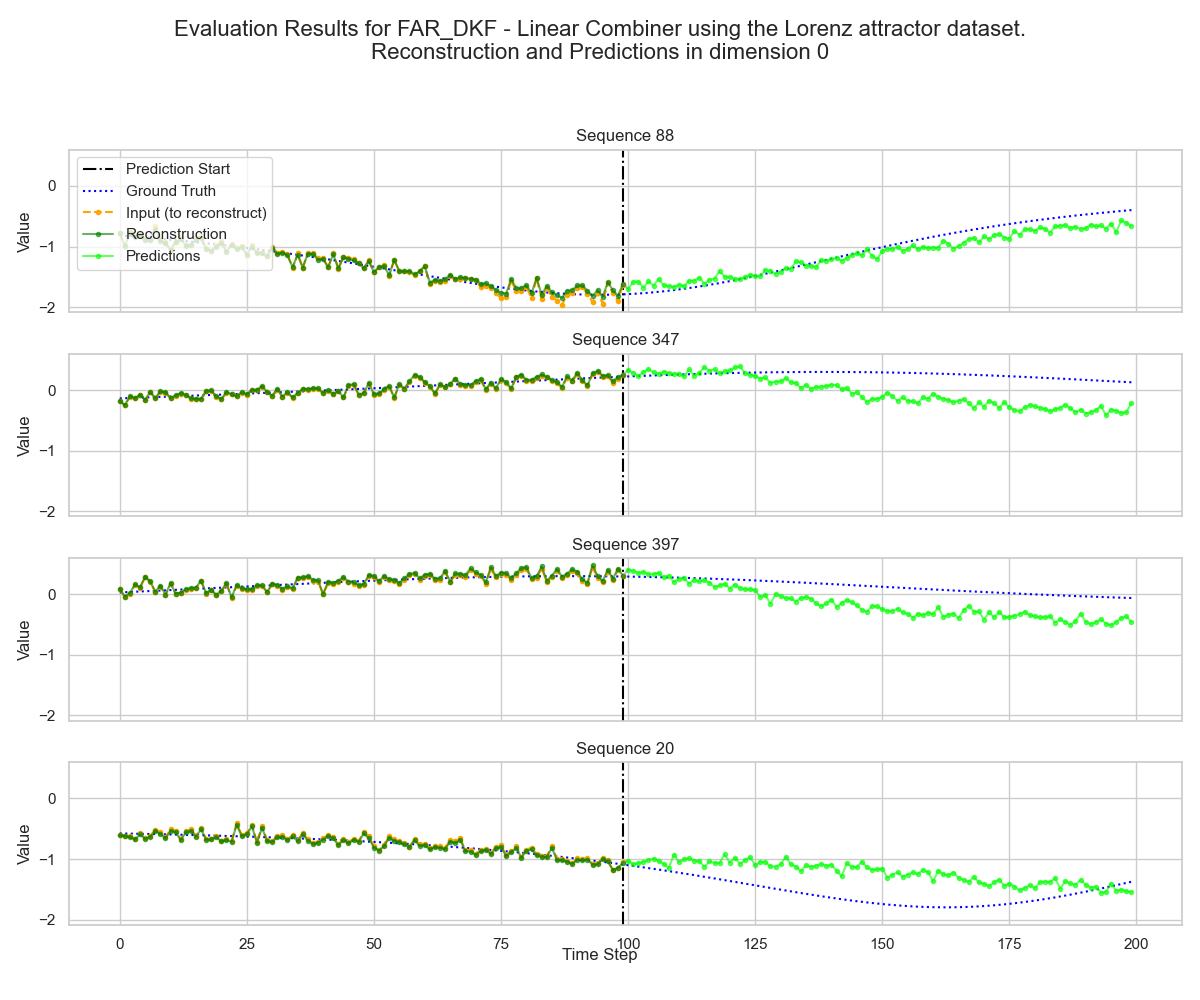
\includegraphics[width=1\textwidth]{./Images/Dataset_3/FAR_DKF_1_dim_0.png}
            \subcaption{Reconstruction and Prediction in the 1st dimension.}
            \label{fig:dataset_3_FAR_DKF_1_dim_0}
        \end{minipage}
        \hfill
        \begin{minipage}{0.31\textwidth}
            \centering
            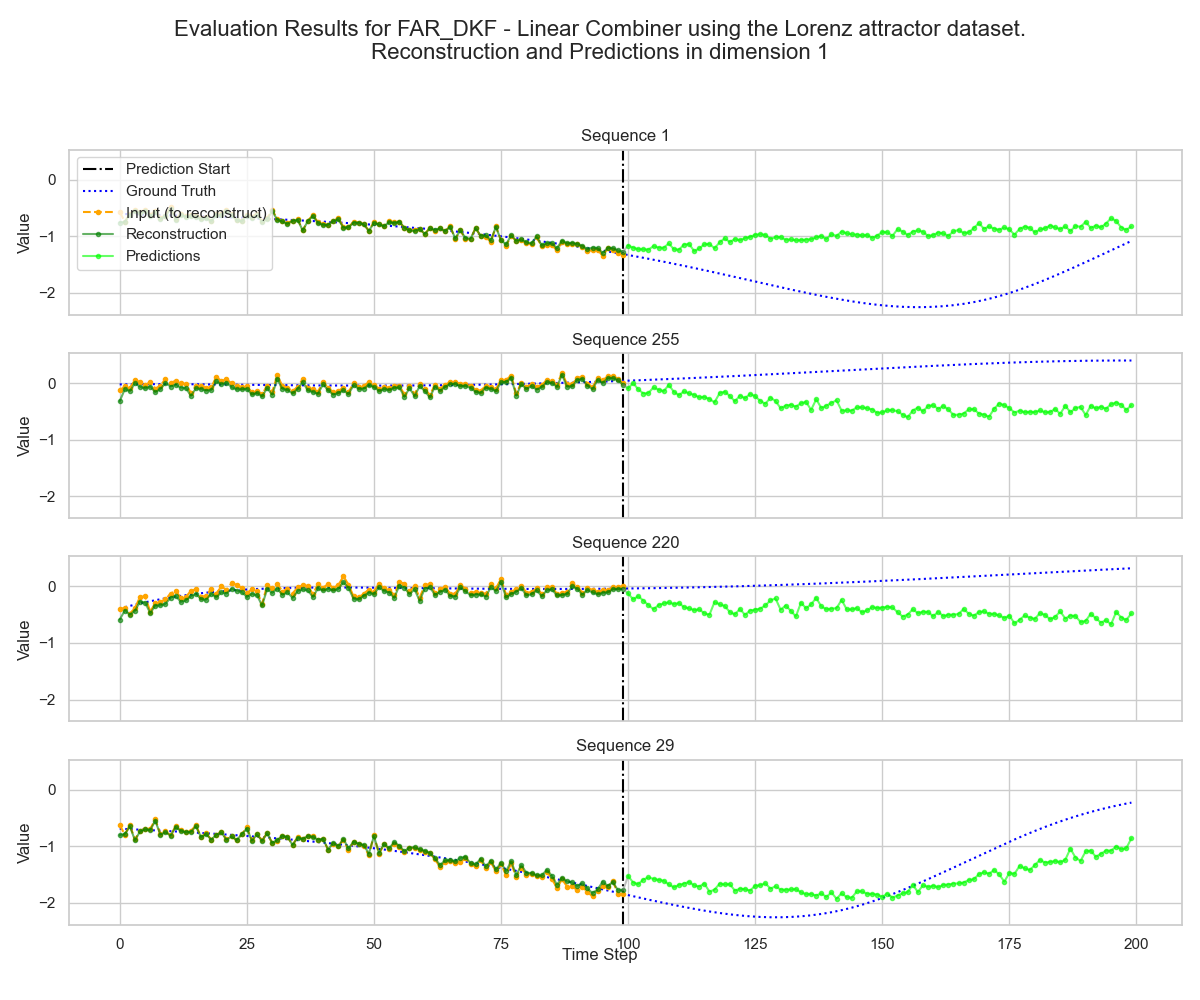
\includegraphics[width=1\textwidth]{./Images/Dataset_3/FAR_DKF_1_dim_1.png}
            \subcaption{Reconstruction and Prediction in the 2nd dimension.}
            \label{fig:dataset_3_FAR_DKF_1_dim_1}
        \end{minipage}
        \hfill
        \begin{minipage}{0.31\textwidth}
            \centering
            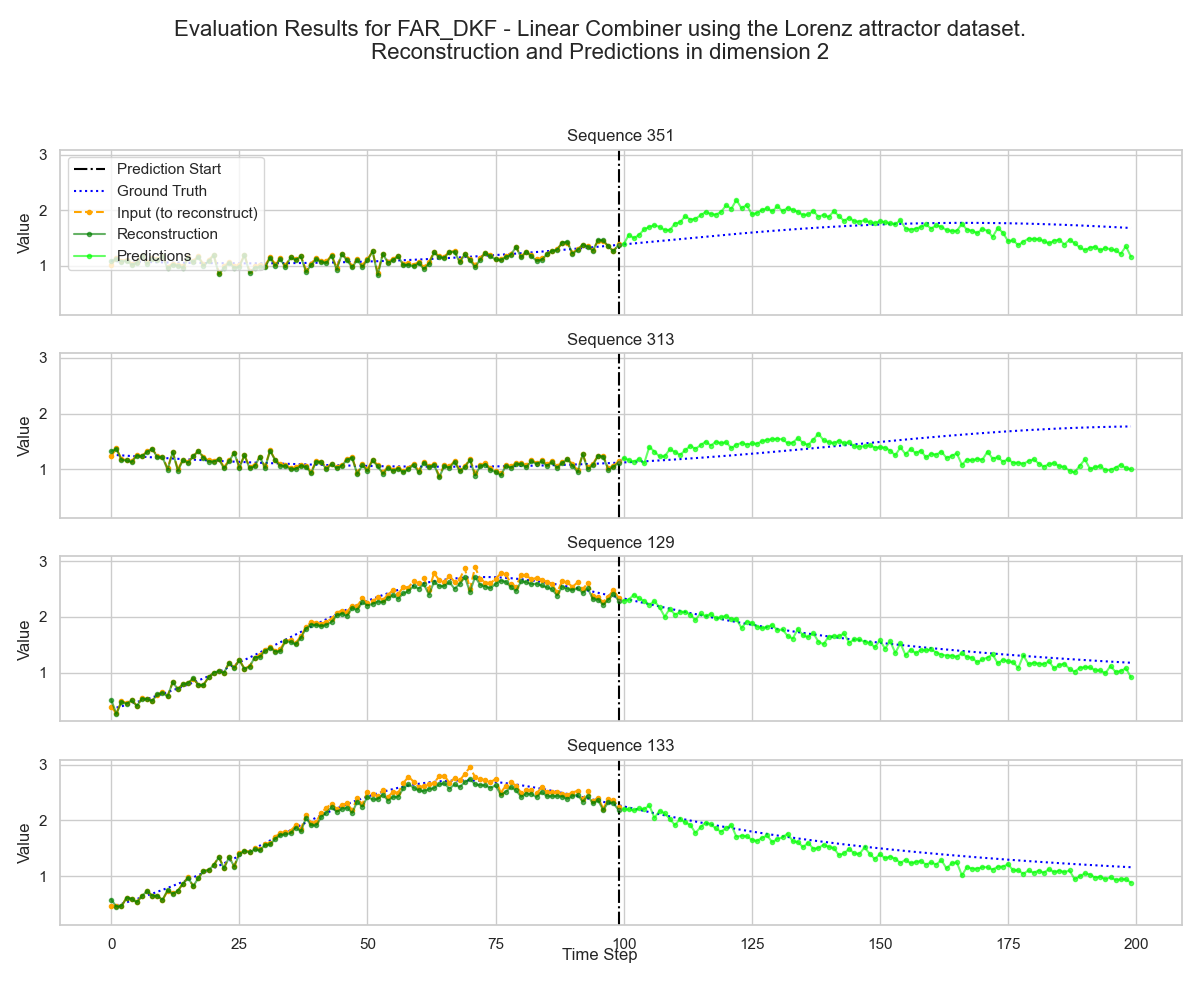
\includegraphics[width=1\textwidth]{./Images/Dataset_3/FAR_DKF_1_dim_2.png}
            \subcaption{Reconstruction and Prediction in the 3rd dimension.}
            \label{fig:dataset_3_FAR_DKF_1_dim_2}
        \end{minipage}
        \caption{Examples of Reconstruction and Prediction for the
        FAR DKF model.}
        \label{fig:dataset_3_FAR_DKF_1_all_dims}
    \end{figure}
    
    \begin{figure}[ht!]
        \centering
        \begin{minipage}{0.31\textwidth}
            \centering
            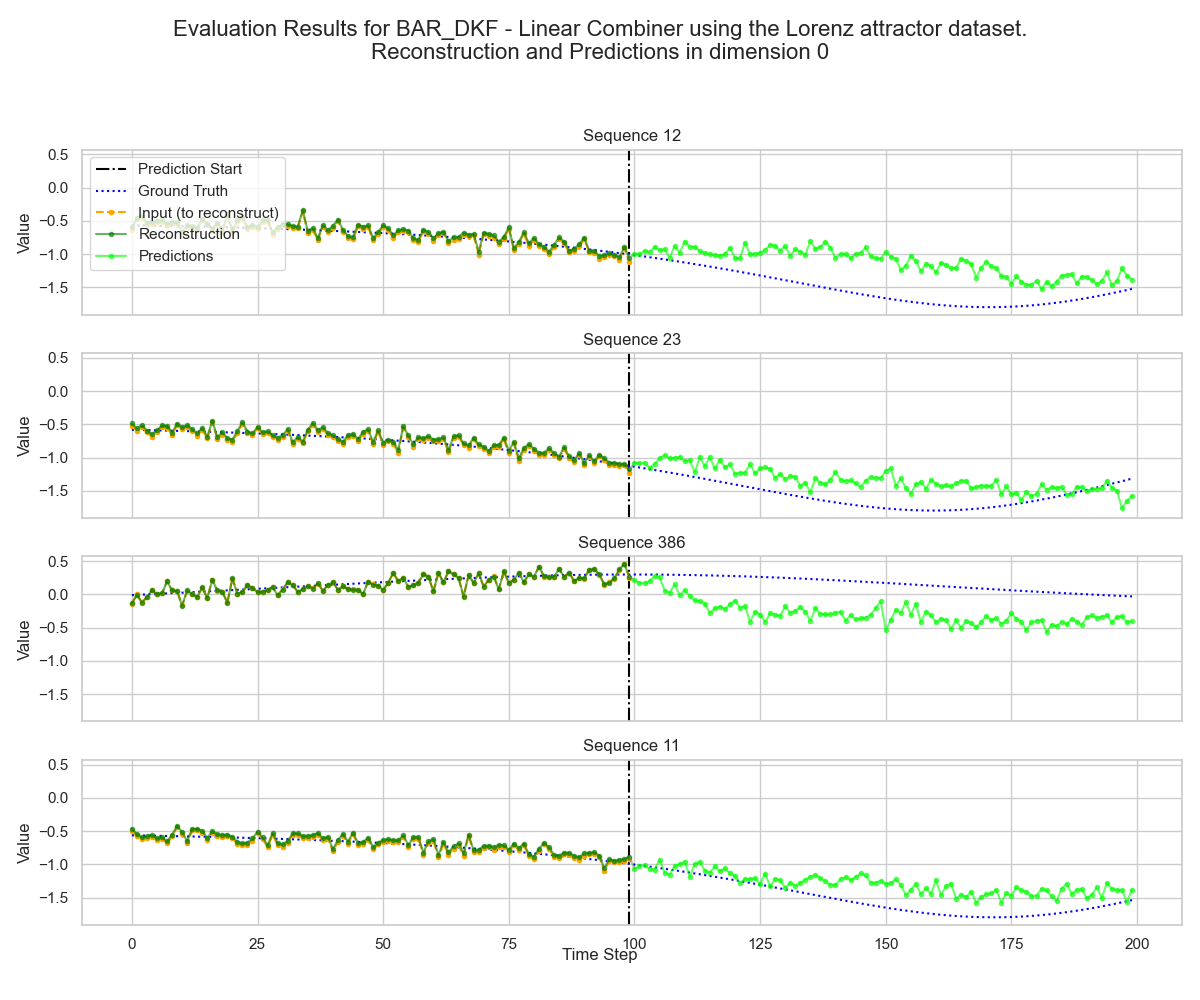
\includegraphics[width=1\textwidth]{./Images/Dataset_3/BAR_DKF_1_dim_0.png}
            \subcaption{Reconstruction and Prediction in the 1st dimension.}
            \label{fig:dataset_3_BAR_DKF_1_dim_0}
        \end{minipage}
        \hfill
        \begin{minipage}{0.31\textwidth}
            \centering
            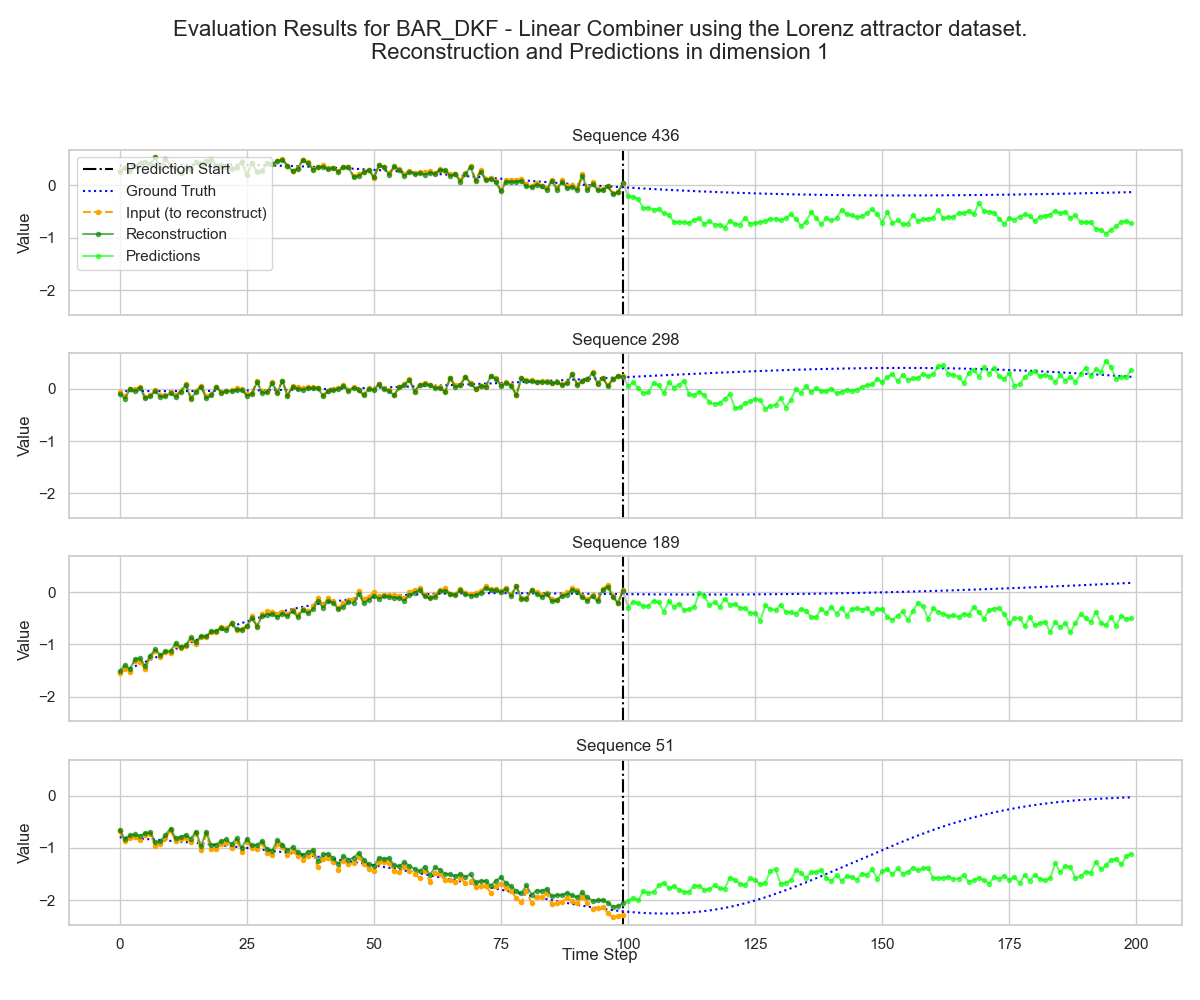
\includegraphics[width=1\textwidth]{./Images/Dataset_3/BAR_DKF_1_dim_1.png}
            \subcaption{Reconstruction and Prediction in the 2nd dimension.}
            \label{fig:dataset_3_BAR_DKF_1_dim_1}
        \end{minipage}
        \hfill
        \begin{minipage}{0.31\textwidth}
            \centering
            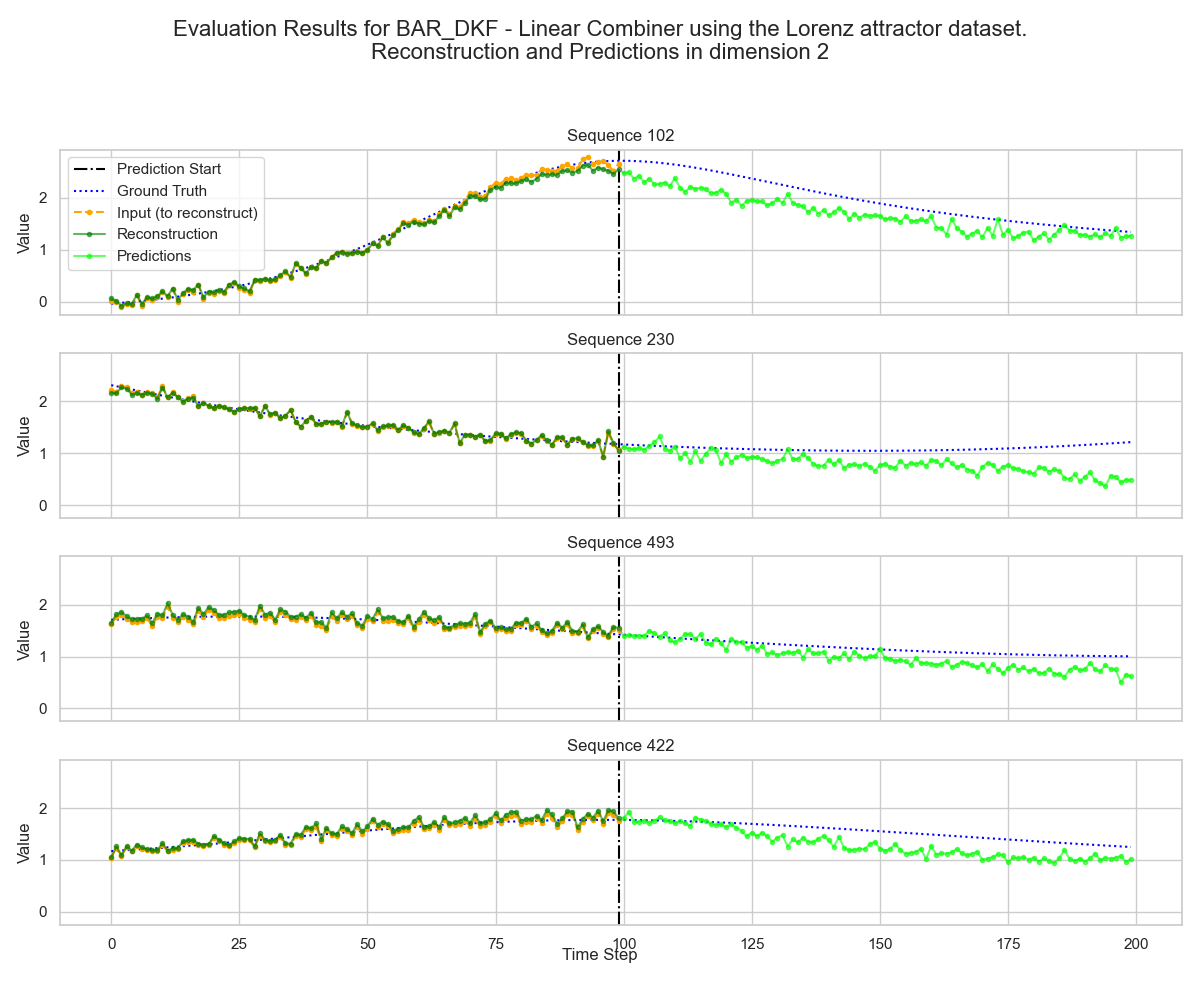
\includegraphics[width=1\textwidth]{./Images/Dataset_3/BAR_DKF_1_dim_2.png}
            \subcaption{Reconstruction and Prediction in the 3rd dimension.}
            \label{fig:dataset_3_BAR_DKF_1_dim_2}
        \end{minipage}
        \caption{Examples of Reconstruction and Prediction for the
        BAR DKF model.}
        \label{fig:dataset_3_BAR_DKF_1_all_dims}
    \end{figure}
    
    \begin{figure}[ht!]
        \centering
        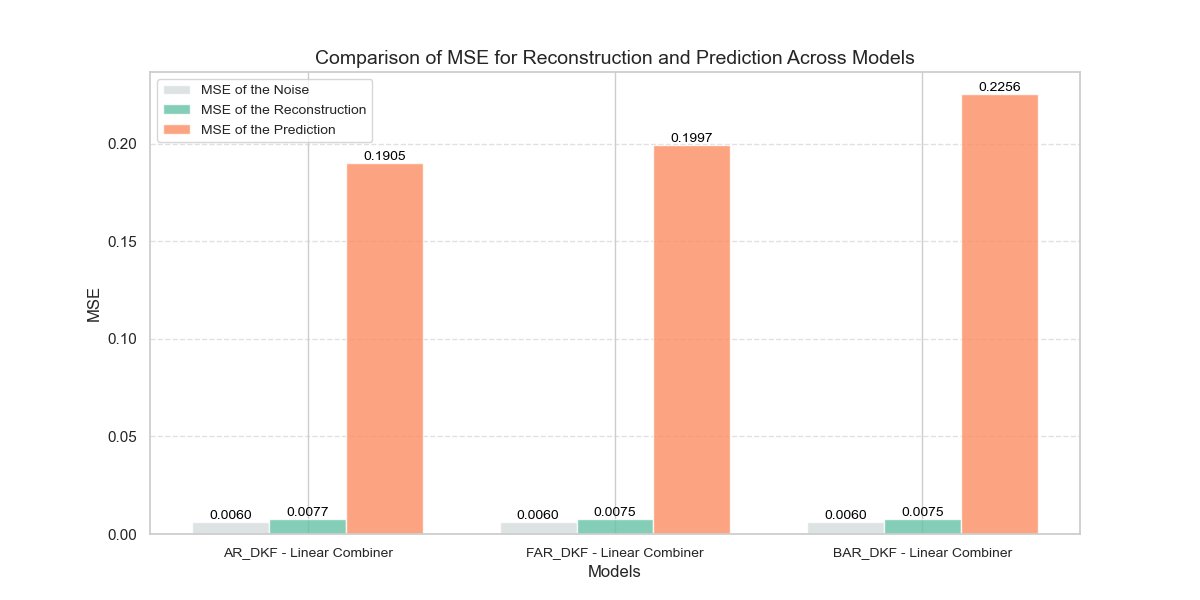
\includegraphics[width=0.75\textwidth]
        {./Images/Dataset_3/mse_comparison.png}
        \caption{Reconstruction and Prediction MSE Comparison for
        AR DKF, FAR DKF, and BAR DKF
        on dataset 3.}
        \label{fig:dataset_3_mse_comparison}
    \end{figure}
    
    \begin{figure}[ht!]
        \centering
        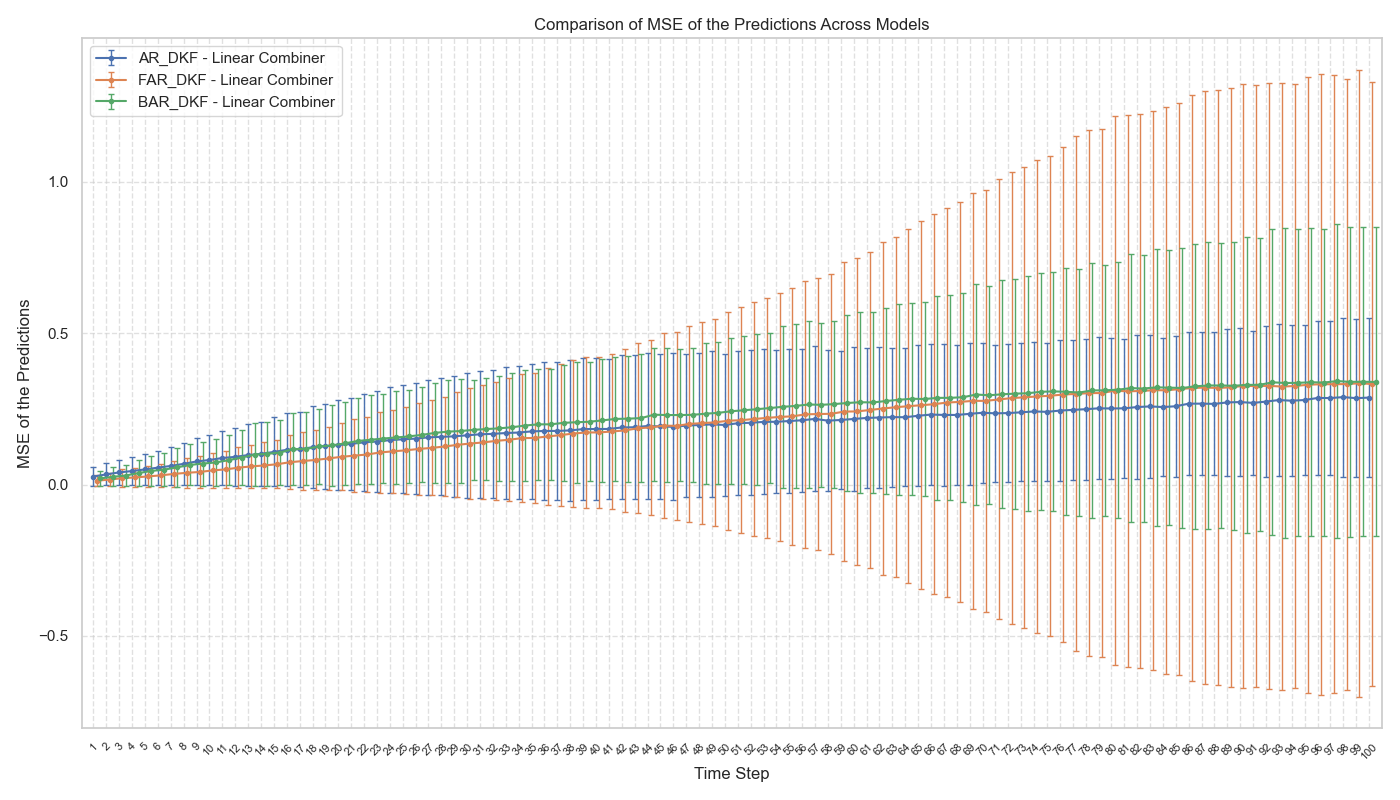
\includegraphics[width=1\textwidth]
        {./Images/Dataset_3/mse_pred_comparison.png}
        \caption{MSE Comparison for AR DKF, FAR DKF, and
        BAR DKF for each prediction points of test sequences of
        dataset 3.}
        \label{fig:dataset_3_mse_pred_comparison}
    \end{figure}

%- - - - - - - - - - - - - - - - - - - - - - - - - - - - - - - - - - - - -
\FloatBarrier
\subsubsection*{Summary of the Lorenz experiments}

The code does not fix a random seed, so each training run starts from
a different initialisation and sees the minibatches in a different
order. Table~\ref{tab:lorenz_mse} gives the forecasting and
reconstruction errors over the four runs of each experiment.

\begin{table}[ht!]
\centering
\small
\begin{tabular}{|c|c|c|c|}
\hline
Dataset & Model & Prediction MSE: mean (std.\ dev.) &
Runs with the lowest error \\ \hline
1 & AR DKF  & 0.0357 (0.0202) & 2 of 4 \\
  & FAR DKF & 0.0315 (0.0063) & 1 of 4 \\
  & BAR DKF & 0.0280 (0.0044) & 1 of 4 \\ \hline
2 & AR DKF  & 0.0244 (0.0135) & 3 of 4 \\
  & FAR DKF & 0.0361 (0.0232) & 1 of 4 \\
  & BAR DKF & 0.0621 (0.0695) & 0 of 4 \\ \hline
3 & AR DKF  & 0.1974 (0.0283) & 1 of 4 \\
  & FAR DKF & 0.1418 (0.0513) & 2 of 4 \\
  & BAR DKF & 0.1711 (0.0597) & 1 of 4 \\ \hline
\end{tabular}
\caption{Lorenz experiments: prediction MSE over four training runs.
The MSE of the noise is 0.0060.}
\label{tab:lorenz_mse}
\end{table}

\begin{itemize}
    \item \textbf{Reconstruction.} In almost every run, all three models
    reconstruct close to the noise level (mean reconstruction MSE between
    0.0050 and 0.0071, except 0.0119 for the AR DKF on dataset 3, due to
    one run at 0.0225). They reproduce the noisy input rather than
    denoise it.
    \item \textbf{Prediction.} The spread between runs of the \emph{same}
    model is as large as the differences between models, and no model is
    consistently best: the AR DKF has the lowest error in three runs out
    of four on dataset 2, the FAR DKF the lowest mean error on dataset 3,
    and on dataset 1 the three means are within one standard deviation of
    each other. The BAR DKF has one poor run on dataset 2 (0.166), which
    drives its mean and spread there. Dataset 3 remains the hardest for
    all models.
\end{itemize}

\subsubsection*{Evaluation of the ELBO on test data}

The theory of Section~\ref{sec:ar_posterior} makes a prediction about
the ELBO, not about forecasting: the FAR DKF and the BAR DKF have
inference networks with the structure of the true posterior
(Proposition~\ref{prop:ar_posterior}); the AR DKF does not. Their gap
$\KL\big(q_\phi \,\|\, p_\theta(\mathbf{z}_{1:T} \mid \mathbf{x}_{1:T})\big)$
between the ELBO and the log-likelihood should therefore be smaller.

To test this, the script \code{evaluate\_elbo.py} evaluates each trained
model on the noisy test sequences (the same noise for all models) with
two quantities, reported per time step:
\begin{itemize}
    \item the ELBO, estimated as during training and averaged over 20
    trajectories per sequence;
    \item the importance-weighted bound \cite{burda2016importance}
    \begin{equation*}
        \mathcal{L}_K = \E\left[\log \frac{1}{K} \sum_{k=1}^{K}
        \frac{p_\theta(\mathbf{x}_{1:T}, \mathbf{z}^{(k)}_{1:T})}
        {q_\phi(\mathbf{z}^{(k)}_{1:T} \mid \mathbf{x}_{1:T})}\right],
        \qquad \mathbf{z}^{(k)}_{1:T} \sim q_\phi(\mathbf{z}_{1:T} \mid
        \mathbf{x}_{1:T}),
    \end{equation*}
    for $K = 1, 10, 100$. It satisfies $\mathcal{L}_1 = \mathcal{L}$
    (the ELBO) and $\mathcal{L}_K \leq \log p_\theta(\mathbf{x}_{1:T})$,
    and it increases with $K$. Hence $\mathcal{L}_{100} - \mathcal{L}$ is
    a \emph{lower bound} on the gap.
\end{itemize}
As a check of the implementation, $\mathcal{L}_1$ agrees with the ELBO
within its confidence interval in every evaluation, and $\mathcal{L}_K$
increases with $K$. The ELBO was evaluated after each of the last three
runs of every dataset (and after the first run for dataset 3).

\begin{table}[ht!]
\centering
\small
\begin{tabular}{|c|c|c|c|}
\hline
Dataset & Model & ELBO: mean (std.\ dev.) &
Gap $\mathcal{L}_{100} - \mathcal{L}$: mean [min, max] \\
\hline
1 & AR DKF  & $-13.8$ (7.5)  & 0.62 [0.58, 0.69] \\
  & FAR DKF & $-23.4$ (8.6)  & 0.65 [0.60, 0.68] \\
  & BAR DKF & $-17.2$ (13.1) & 0.63 [0.56, 0.73] \\ \hline
2 & AR DKF  & $-30.8$ (0.8)  & 0.69 [0.66, 0.70] \\
  & FAR DKF & $-22.9$ (4.7)  & 0.64 [0.62, 0.67] \\
  & BAR DKF & $-25.4$ (12.5) & 0.63 [0.53, 0.69] \\ \hline
3 & AR DKF  & $-41.3$ (8.5)  & 0.80 [0.72, 0.95] \\
  & FAR DKF & $-38.8$ (7.8)  & 0.81 [0.72, 0.95] \\
  & BAR DKF & $-37.5$ (7.4)  & 0.75 [0.73, 0.79] \\ \hline
\end{tabular}
\caption{Lorenz experiments: ELBO and estimated ELBO gap on the test
sequences (in nats per time step; higher ELBO is better). ELBO over
three runs (four for dataset 3); gap over three runs.}
\label{tab:lorenz_elbo}
\end{table}

\begin{itemize}
    \item \textbf{The ELBO varies more between runs than between
    models.} Its standard deviation over runs of the same model is
    mostly between 5 and 13 nats per time step, while the differences between the means
    of the three models are of the same size or smaller, and the model
    with the best ELBO changes from one run to the next. The AR DKF has
    the lowest mean ELBO on dataset 2 (the lowest in two runs out of
    three), yet the lowest forecasting error there: the ELBO and the
    forecasting error measure different things.
    \item \textbf{The estimated gap is the same for the three models}, at
    about 0.6--0.8 nats per time step. With $K = 100$, the
    importance-weighted bound cannot detect the difference that the theory
    predicts. The bound is still rising between $K = 10$ and $K = 100$
    (by 0.2 to 0.4 nats per time step), so it has not converged and the
    true gaps are larger than these estimates. Comparing them would
    require much larger $K$ or a better proposal distribution.
\end{itemize}

\noindent In short, the experiments do not show the advantage of the
FAR DKF and the BAR DKF that the d-separation argument suggests. What
they show clearly is that, at this scale, the variability between
training runs is larger than the differences between the three
inference networks.

\end{appendices}

\annexes
\section{Bayesian Networks: Paths and D-Separation}\label{seq:d_separation}

This is a short overview. A complete treatment is given by Koller and
Friedman \cite{koller2009probabilistic}.

\subsection*{Bayesian networks}

A Bayesian network is a directed acyclic graph (DAG) whose nodes are
random variables, together with the factorisation
\[
    p(v_1, \dots, v_n) = \prod_{k=1}^n p(v_k \mid \mathrm{pa}(v_k)),
\]
where $\mathrm{pa}(v_k)$ are the parents of $v_k$. The graph encodes
conditional independences, which d-separation lets us read directly from
it.

\subsection*{Paths and the three elementary connections}

A \emph{path} between two nodes is a sequence of adjacent nodes,
\textbf{regardless of the direction of the edges}. For example, in
$A \leftarrow B \rightarrow C$ there is a path from $A$ to $C$ even
though no arrow goes from $A$ to $C$. Each intermediate node of a path
takes one of three roles, depending on the two edges that meet at it.

\begin{enumerate}
    \item \textbf{Chain} $A \rightarrow B \rightarrow C$. $A$ influences
    $C$ through $B$.
    \item \textbf{Fork} (common cause) $A \leftarrow B \rightarrow C$.
    $A$ and $C$ are correlated because they share the cause $B$.
    \item \textbf{Collider} (common effect) $A \rightarrow B \leftarrow
    C$. $A$ and $C$ are independent causes of $B$.
\end{enumerate}

\subsection*{Blocked paths}

Let $\mathcal{S}$ be the set of observed (conditioned-on) variables. A
path is \textbf{blocked} by $\mathcal{S}$ if it contains at least one
intermediate node $B$ such that
\begin{itemize}
    \item $B$ is a chain or fork node and $B \in \mathcal{S}$; or
    \item $B$ is a collider and neither $B$ nor any of its descendants is
    in $\mathcal{S}$.
\end{itemize}
Otherwise the path is \textbf{active}. Two sets of variables are
\textbf{d-separated} by $\mathcal{S}$ if every path between them is
blocked. If $\mathcal{X}$ and $\mathcal{Y}$ are d-separated by
$\mathcal{S}$, then $\mathcal{X} \indep \mathcal{Y} \mid \mathcal{S}$ in
every distribution that factorises according to the graph.

\subsection*{The two mechanisms, with examples}

\paragraph{Chains and forks: screening off.}
Observing the middle node of a chain or a fork \emph{blocks} the path.

\emph{Chain.} Let $A$ = \enquote{it rains}, $B$ = \enquote{the grass is
wet}, $C$ = \enquote{someone slips on the grass}:
$A \rightarrow B \rightarrow C$. Without information about the grass,
knowing that it rains makes slipping more likely. But once we know
whether the grass is wet, the rain tells us nothing more about slipping:
all its influence goes through the wetness. Formally,
$p(C \mid A, B) = p(C \mid B)$. The observed $B$ \emph{screens off} $C$
from $A$.

\emph{Fork.} Let $B$ = \enquote{the patient has the flu}, $A$ =
\enquote{fever}, $C$ = \enquote{cough}: $A \leftarrow B \rightarrow C$.
Fever and cough are correlated in the population, because both are
symptoms of the flu. Among patients known to have the flu, observing a
fever does not make a cough more likely: $A \indep C \mid B$.

\paragraph{Colliders: explaining away.}
A collider works the other way round: the path is blocked as long as the
collider is \emph{unobserved}, and observing it (or one of its
descendants) \emph{opens} the path.

Let $A$ = \enquote{it rained}, $C$ = \enquote{the sprinkler was on},
$B$ = \enquote{the grass is wet}: $A \rightarrow B \leftarrow C$. Rain
and sprinkler are independent: $A \indep C$. But once we observe that the
grass is wet, learning that it rained makes the sprinkler \emph{less}
likely, because the rain already explains the wet grass. Observing the
common effect makes its causes dependent. This phenomenon, and only this
one, is called \textbf{explaining away}.

\begin{inwords}
Information flows through chains and forks unless the middle node is
known. It flows through a collider only if the collider (or something it
causes) is known. Two variables are conditionally independent when every
route between them is cut by one of these rules.
\end{inwords}

\subsection*{Application to the DKF}

In the graph of Figure~\ref{fig:dkf_model}, the latent states form a
chain $\mathbf{z}_1 \rightarrow \mathbf{z}_2 \rightarrow \cdots$, each
$\mathbf{z}_t$ has a child $\mathbf{x}_t$, and each input $\mathbf{u}_t$ is
a parent of $\mathbf{z}_t$.
\begin{itemize}
    \item Given $\mathbf{z}_{t-1}$, every path from $\mathbf{x}_{t-1}$,
    $\mathbf{z}_{t-2}$ or $\mathbf{u}_{t-1}$ to $\mathbf{z}_t$ passes
    through $\mathbf{z}_{t-1}$ as a chain or fork node, and is blocked.
    This gives the factorisation of the generative model and the
    structure of the posterior (Sections~\ref{seq:generative_model} and
    \ref{sec:posterior}).
    \item The future observation $\mathbf{x}_{t+1}$ is \emph{not}
    d-separated from $\mathbf{z}_t$ by $\mathbf{z}_{t-1}$: the path
    $\mathbf{z}_t \rightarrow \mathbf{z}_{t+1} \rightarrow
    \mathbf{x}_{t+1}$ is a chain whose middle node is unobserved. This is
    why the inference network needs $\mathbf{x}_{t:T}$.
    \item In the AR DKF, the added edge $\mathbf{x}_{t-1} \rightarrow
    \mathbf{z}_t$ is a path with no intermediate node, which nothing can
    block. This is why the AR DKF posterior depends on past observations
    (Proposition~\ref{prop:ar_posterior}).
\end{itemize}



\bibliographystyle{unsrtnat}
\bibliography{references}

\end{document}
